% Problems, Chapter 8: Waveguides, Resonant Cavities, and Optical Fibers
% Jackson, Classical Electrodynamics, 3rd ed.
% Requires: amsmath, amssymb, tikz

\section*{Problems}

\Needspace{5\baselineskip}
\par\bigskip
\noindent\textbf{8.1}\quad Consider the electric and magnetic fields in the surface region of an excellent conductor in the approximation of Section 8.1, where the skin depth is very small compared to the radii of curvature of the surface or the scale of significant spatial variation of the fields just outside.
\begin{enumerate}
\item[(a)] For a single-frequency component, show that the magnetic field $\mathbf{H}$ and the current density $\mathbf{J}$ are such that $\mathbf{f}$, the time-averaged force per unit area at the surface from the conduction current, is given by
\[
\mathbf{f}=-\mathbf{n}\,\frac{\mu_{c}}{4}\,|\mathbf{H}_{\parallel}|^{2}
\]
where $\mathbf{H}_{\parallel}$ is the peak parallel component of magnetic field at the surface, $\mu_{c}$ is the magnetic permeability of the conductor, and $\mathbf{n}$ is the outward normal at the surface.
\item[(b)] If the magnetic permeability $\mu$ outside the surface is different from $\mu_{c}$, is there an additional magnetic force per unit area? What about electric forces?
\item[(c)] Assume that the fields are a superposition of different frequencies (all high enough that the approximations still hold). Show that the time-averaged force takes the same form as in part a with $|\mathbf{H}_{\parallel}|^{2}$ replaced by $2\langle|\mathbf{H}_{\parallel}|^{2}\rangle$, where the angle brackets $\langle\cdots\rangle$ mean time average.
\end{enumerate}
\solution

Use peak phasors with time dependence $e^{-i\omega t}$ and measure
$u\geq0$ inward from the surface.  Locally the conductor is a
half-space, and the leading skin-layer fields are
\[
\mathbf H(u)=\mathbf H_\parallel e^{-(1-i)u/\delta},\qquad
\mathbf J=\nabla\times\mathbf H
=\frac{1-i}{\delta}\,\mathbf n\times\mathbf H,
\quad \delta=\sqrt{\frac2{\omega\mu_c\sigma}}.
\]
Here $\nabla=-\mathbf n\partial_u$ to this order and displacement
current is negligible compared with $\sigma\mathbf E$.

\textbf{(a)} The time average of the conduction-current force density is
\[
\langle\mathbf J\times\mathbf B\rangle
=\frac{\mu_c}2\operatorname{Re}(\mathbf J\times\mathbf H^*)
=-\frac{\mu_c}{2\delta}\,\mathbf n
|\mathbf H_\parallel|^2e^{-2u/\delta},
\]
where $(\mathbf n\times\mathbf H)\times\mathbf H^*
=-\mathbf n|\mathbf H|^2$ since $\mathbf n\cdot\mathbf H=0$.
Integration through the layer gives
\[
\boxed{\mathbf f=\int_0^\infty\langle\mathbf J\times\mathbf B\rangle du
=-\frac{\mu_c}{4}|\mathbf H_\parallel|^2\mathbf n.}
\]
The result is a magnetic pressure directed into the conductor.

\textbf{(b)} This is only the force from the conduction current.
In the macroscopic Maxwell-stress description, the permeability
jump also produces the magnetic traction
\[
\mathbf f_{\mu}=\frac{\mu_c-\mu}{4}|\mathbf H_\parallel|^2\mathbf n.
\]
One way to see the sign and magnitude is to integrate the magnetic
material-force term $-\tfrac12H^2\nabla\mu$ across the interface:
$\int\nabla\mu\,du_{\rm outward}=(\mu-\mu_c)\mathbf n$ and
$\langle H^2\rangle=|H_\parallel|^2/2$.
Adding the two contributions leaves the exterior magnetic traction
$-\mu|H_\parallel|^2\mathbf n/4$.
The surface charge supplies an outward electric traction
$+\epsilon|E_\perp|^2\mathbf n/4$, to leading order in the
excellent-conductor approximation.  Thus the leading total
macroscopic electromagnetic traction is
\[
\frac14\left(\epsilon|E_\perp|^2-\mu|H_\parallel|^2\right)\mathbf n.
\]
This uses linear, isotropic media and the stated surface approximation;
mechanical stresses of the material are separate from this
 electromagnetic traction.  Tangential electric fields and internal
normal electric fields supply higher-order corrections.

\textbf{(c)} For distinct frequencies, products oscillating at their
sum or difference average to zero over a sufficiently long time.
Combine components of the same frequency into a single phasor first.
For frequency-independent $\mu_c$ in the range considered, summing
(a) gives
\[
\mathbf f=-\frac{\mu_c}{4}\mathbf n\sum_\omega|\mathbf H_\omega|^2
=-\frac{\mu_c}{2}\mathbf n\langle|\mathbf H_\parallel(t)|^2\rangle.
\]
This is the claimed replacement.  If permeability is dispersive,
the first expression instead contains $\mu_c(\omega)$ in each
frequency contribution; it cannot in general be factored out.

\Needspace{5\baselineskip}
\par\bigskip
\noindent\textbf{8.2}\quad A transmission line consisting of two concentric circular cylinders of metal with conductivity $\sigma$ and skin depth $\delta$, as shown, is filled with a uniform lossless dielectric ($\mu$, $\epsilon$). A TEM mode is propagated along this line. Section 8.1 applies.
\begin{enumerate}
\item[(a)] Show that the time-averaged power flow along the line is
\[
P=\sqrt{\frac{\mu}{\epsilon}}\;\pi a^{2}\,|H_{0}|^{2}\,\ln\!\left(\frac{b}{a}\right)
\]
where $H_{0}$ is the peak value of the azimuthal magnetic field at the surface of the inner conductor.
\end{enumerate}

\begin{center}
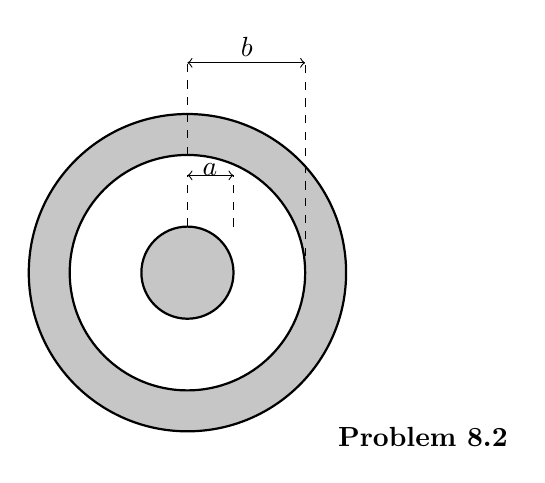
\begin{tikzpicture}[scale=1.3]
  % outer conductor (shaded ring)
  \fill[gray!45,even odd rule] (0,0) circle (1.55) (0,0) circle (1.15);
  \draw[thick] (0,0) circle (1.55);
  \draw[thick] (0,0) circle (1.15);
  % inner conductor (shaded disk)
  \fill[gray!45] (0,0) circle (0.45);
  \draw[thick] (0,0) circle (0.45);
  % b dimension across top
  \draw[<->] (0,2.05) -- (1.15,2.05);
  \draw[dashed] (0,1.15) -- (0,2.05);
  \draw[dashed] (1.15,0) -- (1.15,2.05);
  \node[above] at (0.58,2.02) {$b$};
  % a dimension across inner
  \draw[<->] (0,0.95) -- (0.45,0.95);
  \draw[dashed] (0,0.45) -- (0,0.95);
  \draw[dashed] (0.45,0.45) -- (0.45,0.95);
  \node[above] at (0.22,0.85) {$a$};
  \node at (2.3,-1.6) {\textbf{Problem 8.2}};
\end{tikzpicture}
\end{center}

\begin{enumerate}
\item[(b)] Show that the transmitted power is attenuated along the line as
\[
P(z)=P_{0}e^{-2\gamma z}
\]
where
\[
\gamma=\frac{1}{2\sigma\delta}\sqrt{\frac{\epsilon}{\mu}}\;
\frac{\left(\dfrac{1}{a}+\dfrac{1}{b}\right)}{\ln\left(\dfrac{b}{a}\right)}
\]
\item[(c)] The characteristic impedance $Z_{0}$ of the line is defined as the ratio of the voltage between the cylinders to the axial current flowing in one of them at any position $z$. Show that for this line
\[
Z_{0}=\frac{1}{2\pi}\sqrt{\frac{\mu}{\epsilon}}\,\ln\!\left(\frac{b}{a}\right)
\]
\item[(d)] Show that the series resistance and inductance per unit length of the line are
\begin{align*}
R&=\frac{1}{2\pi\sigma\delta}\left(\frac{1}{a}+\frac{1}{b}\right)\\
L&=\left\{\frac{\mu}{2\pi}\ln\!\left(\frac{b}{a}\right)+\frac{\mu_{c}\delta}{4\pi}\left(\frac{1}{a}+\frac{1}{b}\right)\right\}
\end{align*}
where $\mu_{c}$ is the permeability of the conductor. The correction to the inductance comes from the penetration of the flux into the conductors by a distance of order $\delta$.
\end{enumerate}
\solution

Here $b$ is the radius of the \emph{inner surface} of the outer
conductor.  Set $\eta=\sqrt{\mu/\epsilon}$ and
$R_s=1/(\sigma\delta)$, the surface resistance.  To leading order
in skin depth, the TEM fields in $a<\rho<b$ are
\[
H_\phi(\rho)=\frac{aH_0}{\rho},\qquad E_\rho=\eta H_\phi,
\qquad k=\omega\sqrt{\mu\epsilon}.
\]
Ampere's law fixes $I=2\pi aH_0$, while the radial electrostatic
solution and the plane-wave relation fix $E_\rho$.

\textbf{(a)} With peak phasors the mean axial Poynting flux is
$\eta|H_\phi|^2/2$.  Therefore
\[
P=\frac\eta2\int_a^b\frac{a^2|H_0|^2}{\rho^2}2\pi\rho\,d\rho
=\boxed{\eta\pi a^2|H_0|^2\ln(b/a)}.
\]

\textbf{(b)} The dissipated power per unit length on both surfaces is
\[
P'_\ell=\frac{R_s}2\oint|H_\parallel|^2dl
=\pi R_sa^2|H_0|^2\left(\frac1a+\frac1b\right).
\]
Conservation of energy requires $dP/dz=-P'_\ell=-2\gamma P$.
Dividing by the preceding expression for $P$ gives
\[
\gamma=\frac{R_s}{2\eta}\frac{a^{-1}+b^{-1}}{\ln(b/a)},
\qquad P(z)=P(0)e^{-2\gamma z}.
\]

\textbf{(c)} The voltage magnitude is
$V=\int_a^bE_\rho d\rho=\eta aH_0\ln(b/a)$.  Consequently
\[
\boxed{Z_0=V/I=\frac\eta{2\pi}\ln(b/a).}
\]
It is the leading, real characteristic impedance; conductor losses
produce small complex corrections to the exact impedance.

\textbf{(d)} From $P'_\ell=R|I|^2/2$,
\[
\boxed{R=\frac{R_s}{2\pi}\left(\frac1a+\frac1b\right).}
\]
The average magnetic energy per unit length in the dielectric is
\[
U_{m,\rm ext}=\frac\mu4\int_a^b|H_\phi|^2\,2\pi\rho d\rho
=\frac{\mu\pi a^2|H_0|^2}{2}\ln(b/a).
\]
The penetrating field decays as $e^{-u/\delta}$ in amplitude, giving
\[
U_{m,\rm skin}=\frac{\mu_c}{4}\oint dl\,|H_\parallel|^2
\int_0^\infty e^{-2u/\delta}du
=\frac{\mu_c\delta\pi a^2|H_0|^2}{4}
\left(\frac1a+\frac1b\right).
\]
Using $U_m=L|I|^2/4$ then gives
\[
\boxed{L=\frac\mu{2\pi}\ln(b/a)+
\frac{\mu_c\delta}{4\pi}\left(\frac1a+\frac1b\right).}
\]
As a check, $\omega L_{\rm skin}=R$ because
$\omega\mu_c\delta/2=1/(\sigma\delta)$, the equality of the
resistive and reactive parts of the good-conductor surface impedance.

\Needspace{5\baselineskip}
\par\bigskip
\noindent\textbf{8.3}\quad\begin{enumerate}
\item[(a)] A transmission line consists of two identical thin strips of metal, shown in cross section in the sketch. Assuming that $b\gg a$, discuss the propagation of a TEM mode on this line, repeating the derivations of Problem 8.2. Show that
\begin{align*}
P&=\frac{ab}{2}\sqrt{\frac{\mu}{\epsilon}}\;|H_{0}|^{2}\\[2pt]
\gamma&=\frac{1}{a\sigma\delta}\sqrt{\frac{\epsilon}{\mu}}\\[2pt]
Z_{0}&=\sqrt{\frac{\mu}{\epsilon}}\left(\frac{a}{b}\right)\\[2pt]
R&=\frac{2}{\sigma\delta b}\\[2pt]
L&=\left(\frac{\mu a+\mu_{c}\delta}{b}\right)
\end{align*}
\end{enumerate}

\begin{center}
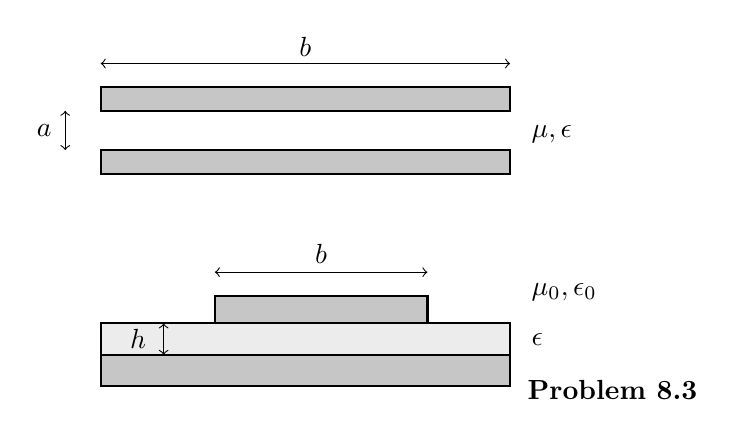
\begin{tikzpicture}[scale=1.0]
  % top figure: two thin strips
  \fill[gray!45] (-0.6,0.75) rectangle (4.6,1.05);
  \draw[thick] (-0.6,0.75) rectangle (4.6,1.05);
  \fill[gray!45] (-0.6,-0.05) rectangle (4.6,0.25);
  \draw[thick] (-0.6,-0.05) rectangle (4.6,0.25);
  \draw[<->] (-0.6,1.35) -- (4.6,1.35);
  \node[above] at (2.0,1.32) {$b$};
  \draw[<->] (-1.05,0.25) -- (-1.05,0.75);
  \node[left] at (-1.1,0.5) {$a$};
  \node[right] at (4.75,0.45) {$\mu,\epsilon$};
  % bottom figure: microstrip
  \fill[gray!45] (-0.6,-2.75) rectangle (4.6,-2.35);
  \draw[thick] (-0.6,-2.75) rectangle (4.6,-2.35);
  \fill[gray!15] (-0.6,-2.35) rectangle (4.6,-1.95);
  \draw[thick] (-0.6,-2.35) rectangle (4.6,-1.95);
  \fill[gray!45] (0.85,-1.95) rectangle (3.55,-1.6);
  \draw[thick] (0.85,-1.95) rectangle (3.55,-1.6);
  \draw[<->] (0.85,-1.3) -- (3.55,-1.3);
  \node[above] at (2.2,-1.32) {$b$};
  \draw[<->] (0.2,-2.35) -- (0.2,-1.95);
  \node[left] at (0.1,-2.15) {$h$};
  \node[right] at (4.75,-1.55) {$\mu_{0},\epsilon_{0}$};
  \node[right] at (4.75,-2.15) {$\epsilon$};
  \node at (5.9,-2.8) {\textbf{Problem 8.3}};
\end{tikzpicture}
\end{center}

\begin{enumerate}
\item[] where the symbols on the left have the same meanings as in Problem 8.2.
\item[(b)] The lower half of the figure shows the cross section of a microstrip line with a strip of width $b$ mounted on a dielectric substrate of thickness $h$ and dielectric constant $\epsilon$, all on a ground plane. What differences occur here compared to part a if $b\gg h$? If $b\ll h$?
\end{enumerate}
\solution

\textbf{(a)} Neglect fringing when $b\gg a$ and assume each metal
strip is thick compared with its skin depth.  In the gap the fields
are uniform, with $E_0=\eta H_0$, where
$\eta=\sqrt{\mu/\epsilon}$.  The voltage and current are
$V=aE_0$ and $I=bH_0$.  The two inner faces carry opposite axial
currents; the exterior field is negligible at this order.  Thus
\[
P=\frac12ab\eta|H_0|^2,\qquad
Z_0=\frac VI=\eta\frac ab.
\]
The two active surfaces dissipate
$P'_\ell=(R_s/2)(2b|H_0|^2)=R_sb|H_0|^2$.
Comparison with $P'_\ell=2\gamma P=R|I|^2/2$ gives
\[
\boxed{\gamma=\frac{R_s}{\eta a}
=\frac1{a\sigma\delta}\sqrt{\frac\epsilon\mu},\qquad
R=\frac{2R_s}{b}=\frac2{\sigma\delta b}.}
\]
The external magnetic energy is $\mu ab|H_0|^2/4$.
The energy in both skin layers is
$(\mu_c/4)(2b|H_0|^2)(\delta/2)=\mu_c\delta b|H_0|^2/4$.
Equating their sum to $L|I|^2/4$ yields
\[
\boxed{L=(\mu a+\mu_c\delta)/b.}
\]
These are all the stated results, with energy velocity
$1/\sqrt{\mu\epsilon}$ to leading order.  ``Thin strips'' means
thin geometrically, not thinner than the penetration depth.

\textbf{(b)} For $b\gg h$, nearly all of the electric and magnetic
energy lies between the strip and the ground plane.  The preceding
parallel-plate formulas apply to leading order with $a=h$ and the
substrate permittivity and permeability; fields at the two strip
edges provide relative corrections that vanish as $h/b\to0$.
For finite $b/h$ the air and substrate have different wave speeds,
so the mode is generally only approximately TEM.

For $b\ll h$ the fields spread transversely over distances of order
$h$, both in the substrate and in the air.  There is no uniform-field
plate region.  In the electrically small, quasi-static limit the
line is described by $Z_0=\sqrt{L'/C'}$ and
$v=1/\sqrt{L'C'}$, where $C'$ is obtained from the two-dielectric
electrostatic problem and $L'$ from the corresponding magnetostatic
problem.  For nonmagnetic media the effective permittivity lies
between $\epsilon_0$ and $\epsilon$; in the very narrow-strip limit
its leading value is $(\epsilon+\epsilon_0)/2$, because the local
field around a strip on the interface occupies two half-spaces.
To see both this average and the logarithmic dependence, let $\lambda$
be charge per unit length and consider $b\ll\rho\ll h$. The two
semicircles in a Gaussian cylinder give
\[
\pi\rho(\epsilon+\epsilon_0)E_\rho\simeq\lambda,
\qquad V\simeq\frac{\lambda}{\pi(\epsilon+\epsilon_0)}\mathcal L,
\qquad \mathcal L=\ln(h/b)+O(1).
\]
The additive constant depends on the near-strip and ground-plane
geometry. Ampere's law gives $H_\phi\simeq I/(2\pi\rho)$ in the
same intermediate region. Integrating its magnetic energy gives
\[
\frac{\mu_0}{4}\int_b^h\left|\frac{I}{2\pi\rho}\right|^2
2\pi\rho\,d\rho\simeq\frac{\mu_0|I|^2}{8\pi}\mathcal L
=\frac{L'|I|^2}{4}.
\]
Thus $C'\simeq\pi(\epsilon+\epsilon_0)/\mathcal L$,
$L'\simeq\mu_0\mathcal L/(2\pi)$, and
\[
v\simeq\frac1{\sqrt{\mu_0(\epsilon+\epsilon_0)/2}},\qquad
Z_0\simeq\frac{\mathcal L}{2\pi}
\sqrt{\frac{2\mu_0}{\epsilon+\epsilon_0}}.
\]
The impedance therefore grows logarithmically with $h/b$. The
strongly nonuniform strip and return currents also
require the surface-loss integral with their actual distributions;
the wide-plate resistance and attenuation formulas no longer apply.
At wavelengths comparable with the transverse dimensions, the
mode has longitudinal field components and geometric dispersion,
so even the quasi-TEM circuit description needs correction.

\Needspace{5\baselineskip}
\par\bigskip
\noindent\textbf{8.4}\quad Transverse electric and magnetic waves are propagated along a hollow, right circular cylinder with inner radius $R$ and conductivity $\sigma$.
\begin{enumerate}
\item[(a)] Find the cutoff frequencies of the various TE and TM modes. Determine numerically the lowest cutoff frequency (the dominant mode) in terms of the tube radius and the ratio of cutoff frequencies of the next four higher modes to that of the dominant mode. For this part assume that the conductivity of the cylinder is infinite.
\item[(b)] Calculate the attenuation constants of the waveguide as a function of frequency for the lowest two distinct modes and plot them as a function of frequency.
\end{enumerate}
\solution

Let $v=1/\sqrt{\mu\epsilon}$ and $\eta=\sqrt{\mu/\epsilon}$ for
the lossless filling (vacuum gives $v=c$).  Write the fields as
$e^{ikz-i\omega t}$, and put $\gamma^2=\omega^2/v^2-k^2$.
Here $\gamma$ is the transverse eigenvalue parameter of (8.34),
and $\beta$ below is the attenuation constant of Section 8.5.
We use $H_z=B_z/\mu$ when evaluating conductor losses; the
constant factor $\mu$ does not change the scalar eigenvalue problem.

\textbf{(a)} Regular longitudinal fields have radial dependence
$J_m(\gamma\rho)$ and angular dependence $\cos m\phi$ or
$\sin m\phi$.  A TM mode has $E_z=0$ on the wall, while a TE
mode has $\partial_\rho H_z=0$ there.  Thus
\[
\boxed{\omega_{c,mn}^{\rm TM}=\frac vR x_{mn},\quad J_m(x_{mn})=0;
\qquad\omega_{c,mn}^{\rm TE}=\frac vR x'_{mn},\quad J_m'(x'_{mn})=0.}
\]
Use positive roots only; the constant Neumann scalar mode does not
produce a nonzero TE electromagnetic field in a hollow guide.
For $m>0$ each family has two angular polarizations.  The first
families, with their cutoffs divided by that of $\mathrm{TE}_{11}$,
are
\[
\begin{array}{c|rr}
\text{family}&\omega_cR/v&\omega_c/\omega_{c,11}^{\rm TE}\\\hline
\mathrm{TE}_{11}&1.841183781&1\\
\mathrm{TM}_{01}&2.404825558&1.306130101\\
\mathrm{TE}_{21}&3.054236928&1.658844141\\
\mathrm{TE}_{01}&3.831705970&2.081109995\\
\mathrm{TM}_{11}&3.831705970&2.081109995\\
\mathrm{TE}_{31}&4.201188941&2.281786850
\end{array}
\]
The middle two families have the same cutoff.  Thus the table gives
both the next four families and, if ``higher'' is counted by distinct
frequency, the next four distinct frequencies.  The dominant cutoff
is $\omega_c=1.841183781v/R$, or $f_c=0.293033v/R$.

\textbf{(b)} Let $R_s=1/(\sigma\delta)=\sqrt{\omega\mu_c/(2\sigma)}$
and denote amplitude attenuation by $\beta$, so power decays as
$e^{-2\beta z}$.  The loss formula is
\[
\beta=\frac{R_s}{4P}\oint|H_\parallel|^2dl.
\]
For clarity, the field and normalization steps behind this formula
are as follows. Maxwell's equations, with the phase convention above,
give the transverse fields in (8.26):
\begin{align*}
\mathbf E_t&=\frac{i}{\gamma^2}
  (k\nabla_tE_z-\omega\mu\widehat{\mathbf z}\times\nabla_tH_z),\\
\mathbf H_t&=\frac{i}{\gamma^2}
  (k\nabla_tH_z+\omega\epsilon\widehat{\mathbf z}\times\nabla_tE_z).
\end{align*}
For either scalar $\psi$, integration by parts and its Dirichlet
or Neumann wall condition imply
\[
\int|\nabla_t\psi|^2dA
=-\int\psi^*\nabla_t^2\psi\,dA
+\oint\psi^*\partial_n\psi\,dl=\gamma^2N,
\qquad N=\int|\psi|^2dA.
\]
Inserting the transverse fields into
$P=\tfrac12\operatorname{Re}\int(\mathbf E_t\times\mathbf H_t^*)
\cdot\widehat{\mathbf z}\,dA$ then supplies the power formulas below.
For a TM field $\psi=E_z$ with $N=\int|\psi|^2dA$,
\[
P=\frac{\omega\epsilon k}{2\gamma^2}N,\qquad
\oint|H_\parallel|^2dl
=\frac{\omega^2\epsilon^2}{\gamma^4}\oint|\partial_n\psi|^2dl.
\]
The radial normalization follows directly from Bessel's equation:
\[
\frac{d}{dx}\left\{x^2J_m'(x)^2+(x^2-m^2)J_m(x)^2\right\}
=2xJ_m(x)^2.
\]
Its integral from $0$ to $\chi=\gamma R$ gives
\[
\int_0^R\rho J_m(\gamma\rho)^2d\rho
=\frac{R^2}{2}\left[J_m'(\chi)^2+
\left(1-\frac{m^2}{\chi^2}\right)J_m(\chi)^2\right].
\]
At a TM zero, the angular factor cancels between the area integral
and the boundary integral $R\gamma^2J_m'(\chi)^2$ times that factor.
This gives
$\oint|\partial_n\psi|^2dl=2\gamma^2N/R$.  Hence
\[
\boxed{\beta_{\rm TM}=
\frac{R_s}{\eta R\sqrt{1-(\omega_c/\omega)^2}}.}
\]
For TE modes put $\psi=H_z$.  At the wall the longitudinal field
and the tangential transverse field both contribute:
\[
P=\frac{\omega\mu k}{2\gamma^2}N,\qquad
\oint|H_\parallel|^2dl
=\oint\left(|\psi|^2+\frac{k^2}{\gamma^4}|\partial_s\psi|^2\right)dl.
\]
For $\chi=x'_{mn}$ the Bessel norm and the angular derivative give
\[
\frac{\oint|\psi|^2dl}{N}=\frac{2}{R(1-m^2/\chi^2)},\qquad
\oint|\partial_s\psi|^2dl=\frac{m^2}{R^2}\oint|\psi|^2dl.
\]
Substitute $k^2=(\omega/v)^2-\chi^2/R^2$. To display the
simplification, put $t=\omega_c/\omega$; the dimensionless factor is
\[
\frac{t^2}{1-m^2/\chi^2}
\left[1+\frac{m^2}{\chi^2}\frac{1-t^2}{t^2}\right]
=t^2+\frac{m^2}{\chi^2-m^2}.
\]
Therefore
\[
\boxed{\beta_{{\rm TE},mn}=
\frac{R_s}{\eta R\sqrt{1-(\omega_c/\omega)^2}}
\left[\left(\frac{\omega_c}{\omega}\right)^2+
\frac{m^2}{\chi^2-m^2}\right].}
\]
Use $m=1$, $\chi=1.841183781$ for the lowest TE mode, and the
TM formula with $\omega_cR/v=2.404825558$ for the next distinct
mode.  The plot retains $R_s\propto\sqrt\omega$; the normalization
uses its value at the dominant cutoff.
\begin{center}\begin{tikzpicture}[x=1cm,y=1cm,>=stealth]
\draw[->] (0,0)--(10.2,0);
\draw[->] (0,0)--(0,5.2);
\draw (0.00000,.06)--(0.00000,-.06) node[below] {\scriptsize $1$};
\draw (1.42857,.06)--(1.42857,-.06) node[below] {\scriptsize $2$};
\draw (2.85714,.06)--(2.85714,-.06) node[below] {\scriptsize $3$};
\draw (4.28571,.06)--(4.28571,-.06) node[below] {\scriptsize $4$};
\draw (5.71429,.06)--(5.71429,-.06) node[below] {\scriptsize $5$};
\draw (7.14286,.06)--(7.14286,-.06) node[below] {\scriptsize $6$};
\draw (8.57143,.06)--(8.57143,-.06) node[below] {\scriptsize $7$};
\draw (10.00000,.06)--(10.00000,-.06) node[below] {\scriptsize $8$};
\draw (.06,0.00000)--(-.06,0.00000) node[left] {\scriptsize $0$};
\draw (.06,1.25000)--(-.06,1.25000) node[left] {\scriptsize $2$};
\draw (.06,2.50000)--(-.06,2.50000) node[left] {\scriptsize $4$};
\draw (.06,3.75000)--(-.06,3.75000) node[left] {\scriptsize $6$};
\draw (.06,5.00000)--(-.06,5.00000) node[left] {\scriptsize $8$};
\node[below] at (5.0,-.45) {$\omega/\omega_{c,11}^{\rm TE}$};
\node[rotate=90] at (-.75,2.5) {$\beta\eta R/R_s(\omega_{c,11}^{\rm TE})$};
\begin{scope}
\clip (0,0) rectangle (10,5);
\draw[blue,thick] plot coordinates {(0.007143,8.858114) (0.027169,4.532437) (0.047194,3.432258) (0.067220,2.870807) (0.087246,2.515807) (0.107272,2.265524) (0.127297,2.076951) (0.147323,1.928357) (0.167349,1.807417) (0.187375,1.706553) (0.207401,1.620812) (0.227426,1.546801) (0.247452,1.482110) (0.267478,1.424969) (0.287504,1.374048) (0.307529,1.328323) (0.327555,1.286994) (0.347581,1.249422) (0.367607,1.215091) (0.387632,1.183582) (0.407658,1.154545) (0.427684,1.127690) (0.447710,1.102773) (0.467735,1.079584) (0.487761,1.057946) (0.507787,1.037706) (0.527813,1.018730) (0.547839,1.000904) (0.567864,0.984124) (0.587890,0.968301) (0.607916,0.953358) (0.627942,0.939222) (0.647967,0.925832) (0.667993,0.913131) (0.688019,0.901070) (0.708045,0.889601) (0.728070,0.878685) (0.748096,0.868284) (0.768122,0.858365) (0.788148,0.848896) (0.808173,0.839849) (0.828199,0.831199) (0.848225,0.822921) (0.868251,0.814995) (0.888277,0.807399) (0.908302,0.800116) (0.928328,0.793128) (0.948354,0.786420) (0.968380,0.779977) (0.988405,0.773784) (1.008431,0.767830) (1.028457,0.762103) (1.048483,0.756591) (1.068508,0.751284) (1.088534,0.746172) (1.108560,0.741247) (1.128586,0.736500) (1.148612,0.731922) (1.168637,0.727507) (1.188663,0.723247) (1.208689,0.719136) (1.228715,0.715167) (1.248740,0.711334) (1.268766,0.707632) (1.288792,0.704056) (1.308818,0.700600) (1.328843,0.697259) (1.348869,0.694031) (1.368895,0.690909) (1.388921,0.687890) (1.408946,0.684970) (1.428972,0.682145) (1.448998,0.679412) (1.469024,0.676768) (1.489050,0.674210) (1.509075,0.671734) (1.529101,0.669337) (1.549127,0.667018) (1.569153,0.664772) (1.589178,0.662599) (1.609204,0.660494) (1.629230,0.658457) (1.649256,0.656485) (1.669281,0.654575) (1.689307,0.652726) (1.709333,0.650936) (1.729359,0.649203) (1.749384,0.647525) (1.769410,0.645901) (1.789436,0.644328) (1.809462,0.642806) (1.829488,0.641333) (1.849513,0.639907) (1.869539,0.638527) (1.889565,0.637191) (1.909591,0.635900) (1.929616,0.634650) (1.949642,0.633441) (1.969668,0.632272) (1.989694,0.631141) (2.009719,0.630048) (2.029745,0.628992) (2.049771,0.627971) (2.069797,0.626985) (2.089823,0.626032) (2.109848,0.625112) (2.129874,0.624225) (2.149900,0.623368) (2.169926,0.622541) (2.189951,0.621744) (2.209977,0.620976) (2.230003,0.620235) (2.250029,0.619522) (2.270054,0.618835) (2.290080,0.618175) (2.310106,0.617539) (2.330132,0.616929) (2.350157,0.616342) (2.370183,0.615779) (2.390209,0.615239) (2.410235,0.614721) (2.430261,0.614224) (2.450286,0.613750) (2.470312,0.613295) (2.490338,0.612862) (2.510364,0.612448) (2.530389,0.612053) (2.550415,0.611677) (2.570441,0.611320) (2.590467,0.610981) (2.610492,0.610660) (2.630518,0.610355) (2.650544,0.610068) (2.670570,0.609797) (2.690595,0.609543) (2.710621,0.609304) (2.730647,0.609080) (2.750673,0.608872) (2.770699,0.608678) (2.790724,0.608499) (2.810750,0.608334) (2.830776,0.608182) (2.850802,0.608045) (2.870827,0.607920) (2.890853,0.607809) (2.910879,0.607710) (2.930905,0.607623) (2.950930,0.607549) (2.970956,0.607487) (2.990982,0.607436) (3.011008,0.607397) (3.031033,0.607369) (3.051059,0.607352) (3.071085,0.607346) (3.091111,0.607350) (3.111137,0.607365) (3.131162,0.607389) (3.151188,0.607424) (3.171214,0.607468) (3.191240,0.607522) (3.211265,0.607585) (3.231291,0.607658) (3.251317,0.607739) (3.271343,0.607829) (3.291368,0.607928) (3.311394,0.608035) (3.331420,0.608150) (3.351446,0.608274) (3.371472,0.608406) (3.391497,0.608545) (3.411523,0.608692) (3.431549,0.608847) (3.451575,0.609009) (3.471600,0.609178) (3.491626,0.609355) (3.511652,0.609538) (3.531678,0.609728) (3.551703,0.609925) (3.571729,0.610129) (3.591755,0.610339) (3.611781,0.610555) (3.631806,0.610778) (3.651832,0.611007) (3.671858,0.611242) (3.691884,0.611482) (3.711910,0.611729) (3.731935,0.611981) (3.751961,0.612239) (3.771987,0.612503) (3.792013,0.612771) (3.812038,0.613045) (3.832064,0.613325) (3.852090,0.613609) (3.872116,0.613898) (3.892141,0.614193) (3.912167,0.614492) (3.932193,0.614796) (3.952219,0.615104) (3.972244,0.615418) (3.992270,0.615735) (4.012296,0.616057) (4.032322,0.616384) (4.052348,0.616715) (4.072373,0.617050) (4.092399,0.617389) (4.112425,0.617732) (4.132451,0.618079) (4.152476,0.618430) (4.172502,0.618785) (4.192528,0.619144) (4.212554,0.619507) (4.232579,0.619873) (4.252605,0.620243) (4.272631,0.620616) (4.292657,0.620993) (4.312683,0.621373) (4.332708,0.621757) (4.352734,0.622143) (4.372760,0.622534) (4.392786,0.622927) (4.412811,0.623323) (4.432837,0.623723) (4.452863,0.624125) (4.472889,0.624531) (4.492914,0.624939) (4.512940,0.625351) (4.532966,0.625765) (4.552992,0.626182) (4.573017,0.626602) (4.593043,0.627024) (4.613069,0.627449) (4.633095,0.627877) (4.653121,0.628307) (4.673146,0.628740) (4.693172,0.629175) (4.713198,0.629613) (4.733224,0.630053) (4.753249,0.630496) (4.773275,0.630941) (4.793301,0.631388) (4.813327,0.631837) (4.833352,0.632289) (4.853378,0.632742) (4.873404,0.633198) (4.893430,0.633656) (4.913455,0.634116) (4.933481,0.634578) (4.953507,0.635042) (4.973533,0.635508) (4.993559,0.635976) (5.013584,0.636446) (5.033610,0.636918) (5.053636,0.637391) (5.073662,0.637866) (5.093687,0.638344) (5.113713,0.638822) (5.133739,0.639303) (5.153765,0.639785) (5.173790,0.640269) (5.193816,0.640755) (5.213842,0.641242) (5.233868,0.641731) (5.253894,0.642221) (5.273919,0.642713) (5.293945,0.643206) (5.313971,0.643701) (5.333997,0.644197) (5.354022,0.644695) (5.374048,0.645194) (5.394074,0.645695) (5.414100,0.646197) (5.434125,0.646700) (5.454151,0.647205) (5.474177,0.647710) (5.494203,0.648217) (5.514228,0.648726) (5.534254,0.649235) (5.554280,0.649746) (5.574306,0.650258) (5.594332,0.650771) (5.614357,0.651286) (5.634383,0.651801) (5.654409,0.652318) (5.674435,0.652835) (5.694460,0.653354) (5.714486,0.653874) (5.734512,0.654395) (5.754538,0.654917) (5.774563,0.655439) (5.794589,0.655963) (5.814615,0.656488) (5.834641,0.657014) (5.854666,0.657540) (5.874692,0.658068) (5.894718,0.658597) (5.914744,0.659126) (5.934770,0.659656) (5.954795,0.660187) (5.974821,0.660719) (5.994847,0.661252) (6.014873,0.661786) (6.034898,0.662320) (6.054924,0.662855) (6.074950,0.663391) (6.094976,0.663928) (6.115001,0.664466) (6.135027,0.665004) (6.155053,0.665543) (6.175079,0.666082) (6.195104,0.666623) (6.215130,0.667164) (6.235156,0.667705) (6.255182,0.668248) (6.275208,0.668791) (6.295233,0.669334) (6.315259,0.669879) (6.335285,0.670423) (6.355311,0.670969) (6.375336,0.671515) (6.395362,0.672061) (6.415388,0.672609) (6.435414,0.673156) (6.455439,0.673705) (6.475465,0.674253) (6.495491,0.674803) (6.515517,0.675352) (6.535543,0.675903) (6.555568,0.676453) (6.575594,0.677005) (6.595620,0.677557) (6.615646,0.678109) (6.635671,0.678661) (6.655697,0.679215) (6.675723,0.679768) (6.695749,0.680322) (6.715774,0.680876) (6.735800,0.681431) (6.755826,0.681986) (6.775852,0.682542) (6.795877,0.683098) (6.815903,0.683654) (6.835929,0.684211) (6.855955,0.684768) (6.875981,0.685326) (6.896006,0.685883) (6.916032,0.686441) (6.936058,0.687000) (6.956084,0.687559) (6.976109,0.688118) (6.996135,0.688677) (7.016161,0.689237) (7.036187,0.689797) (7.056212,0.690357) (7.076238,0.690917) (7.096264,0.691478) (7.116290,0.692039) (7.136315,0.692600) (7.156341,0.693162) (7.176367,0.693724) (7.196393,0.694286) (7.216419,0.694848) (7.236444,0.695411) (7.256470,0.695973) (7.276496,0.696536) (7.296522,0.697099) (7.316547,0.697663) (7.336573,0.698226) (7.356599,0.698790) (7.376625,0.699354) (7.396650,0.699918) (7.416676,0.700482) (7.436702,0.701047) (7.456728,0.701611) (7.476754,0.702176) (7.496779,0.702741) (7.516805,0.703306) (7.536831,0.703871) (7.556857,0.704437) (7.576882,0.705002) (7.596908,0.705568) (7.616934,0.706133) (7.636960,0.706699) (7.656985,0.707265) (7.677011,0.707831) (7.697037,0.708397) (7.717063,0.708963) (7.737088,0.709530) (7.757114,0.710096) (7.777140,0.710663) (7.797166,0.711229) (7.817192,0.711796) (7.837217,0.712363) (7.857243,0.712930) (7.877269,0.713496) (7.897295,0.714063) (7.917320,0.714630) (7.937346,0.715197) (7.957372,0.715765) (7.977398,0.716332) (7.997423,0.716899) (8.017449,0.717466) (8.037475,0.718033) (8.057501,0.718601) (8.077526,0.719168) (8.097552,0.719735) (8.117578,0.720303) (8.137604,0.720870) (8.157630,0.721438) (8.177655,0.722005) (8.197681,0.722572) (8.217707,0.723140) (8.237733,0.723707) (8.257758,0.724275) (8.277784,0.724842) (8.297810,0.725409) (8.317836,0.725977) (8.337861,0.726544) (8.357887,0.727111) (8.377913,0.727679) (8.397939,0.728246) (8.417965,0.728813) (8.437990,0.729381) (8.458016,0.729948) (8.478042,0.730515) (8.498068,0.731082) (8.518093,0.731649) (8.538119,0.732216) (8.558145,0.732783) (8.578171,0.733350) (8.598196,0.733917) (8.618222,0.734484) (8.638248,0.735051) (8.658274,0.735618) (8.678299,0.736184) (8.698325,0.736751) (8.718351,0.737317) (8.738377,0.737884) (8.758403,0.738450) (8.778428,0.739017) (8.798454,0.739583) (8.818480,0.740149) (8.838506,0.740715) (8.858531,0.741281) (8.878557,0.741847) (8.898583,0.742413) (8.918609,0.742979) (8.938634,0.743545) (8.958660,0.744110) (8.978686,0.744676) (8.998712,0.745241) (9.018737,0.745806) (9.038763,0.746372) (9.058789,0.746937) (9.078815,0.747502) (9.098841,0.748067) (9.118866,0.748631) (9.138892,0.749196) (9.158918,0.749761) (9.178944,0.750325) (9.198969,0.750889) (9.218995,0.751454) (9.239021,0.752018) (9.259047,0.752582) (9.279072,0.753145) (9.299098,0.753709) (9.319124,0.754273) (9.339150,0.754836) (9.359175,0.755400) (9.379201,0.755963) (9.399227,0.756526) (9.419253,0.757089) (9.439279,0.757652) (9.459304,0.758214) (9.479330,0.758777) (9.499356,0.759339) (9.519382,0.759902) (9.539407,0.760464) (9.559433,0.761026) (9.579459,0.761588) (9.599485,0.762149) (9.619510,0.762711) (9.639536,0.763272) (9.659562,0.763834) (9.679588,0.764395) (9.699614,0.764956) (9.719639,0.765517) (9.739665,0.766077) (9.759691,0.766638) (9.779717,0.767198) (9.799742,0.767758) (9.819768,0.768318) (9.839794,0.768878) (9.859820,0.769438) (9.879845,0.769998) (9.899871,0.770557) (9.919897,0.771116) (9.939923,0.771675) (9.959948,0.772234) (9.979974,0.772793) (10.000000,0.773351)};
\draw[red,dashed,thick] plot coordinates {(0.446658,7.187538) (0.466603,4.111562) (0.486547,3.212589) (0.506491,2.745297) (0.526436,2.449699) (0.546380,2.242511) (0.566324,2.087774) (0.586269,1.967103) (0.606213,1.870000) (0.626157,1.789983) (0.646102,1.722807) (0.666046,1.665561) (0.685990,1.616175) (0.705935,1.573132) (0.725879,1.535292) (0.745823,1.501780) (0.765768,1.471911) (0.785712,1.445141) (0.805656,1.421034) (0.825601,1.399230) (0.845545,1.379437) (0.865489,1.361408) (0.885434,1.344938) (0.905378,1.329853) (0.925323,1.316002) (0.945267,1.303259) (0.965211,1.291513) (0.985156,1.280668) (1.005100,1.270640) (1.025044,1.261356) (1.044989,1.252750) (1.064933,1.244766) (1.084877,1.237352) (1.104822,1.230462) (1.124766,1.224056) (1.144710,1.218096) (1.164655,1.212551) (1.184599,1.207391) (1.204543,1.202587) (1.224488,1.198116) (1.244432,1.193956) (1.264376,1.190085) (1.284321,1.186486) (1.304265,1.183141) (1.324209,1.180035) (1.344154,1.177153) (1.364098,1.174482) (1.384042,1.172009) (1.403987,1.169723) (1.423931,1.167615) (1.443876,1.165673) (1.463820,1.163889) (1.483764,1.162254) (1.503709,1.160761) (1.523653,1.159403) (1.543597,1.158172) (1.563542,1.157061) (1.583486,1.156066) (1.603430,1.155181) (1.623375,1.154399) (1.643319,1.153717) (1.663263,1.153130) (1.683208,1.152632) (1.703152,1.152221) (1.723096,1.151892) (1.743041,1.151642) (1.762985,1.151466) (1.782929,1.151363) (1.802874,1.151328) (1.822818,1.151359) (1.842762,1.151454) (1.862707,1.151608) (1.882651,1.151821) (1.902595,1.152089) (1.922540,1.152411) (1.942484,1.152784) (1.962429,1.153206) (1.982373,1.153675) (2.002317,1.154189) (2.022262,1.154748) (2.042206,1.155348) (2.062150,1.155989) (2.082095,1.156668) (2.102039,1.157385) (2.121983,1.158138) (2.141928,1.158926) (2.161872,1.159747) (2.181816,1.160600) (2.201761,1.161485) (2.221705,1.162399) (2.241649,1.163343) (2.261594,1.164314) (2.281538,1.165312) (2.301482,1.166336) (2.321427,1.167385) (2.341371,1.168459) (2.361315,1.169556) (2.381260,1.170675) (2.401204,1.171816) (2.421148,1.172978) (2.441093,1.174161) (2.461037,1.175363) (2.480982,1.176584) (2.500926,1.177824) (2.520870,1.179082) (2.540815,1.180356) (2.560759,1.181648) (2.580703,1.182955) (2.600648,1.184278) (2.620592,1.185616) (2.640536,1.186969) (2.660481,1.188336) (2.680425,1.189717) (2.700369,1.191110) (2.720314,1.192517) (2.740258,1.193936) (2.760202,1.195367) (2.780147,1.196809) (2.800091,1.198263) (2.820035,1.199728) (2.839980,1.201203) (2.859924,1.202689) (2.879868,1.204184) (2.899813,1.205689) (2.919757,1.207204) (2.939701,1.208727) (2.959646,1.210259) (2.979590,1.211800) (2.999535,1.213348) (3.019479,1.214905) (3.039423,1.216469) (3.059368,1.218041) (3.079312,1.219620) (3.099256,1.221205) (3.119201,1.222798) (3.139145,1.224397) (3.159089,1.226002) (3.179034,1.227614) (3.198978,1.229231) (3.218922,1.230855) (3.238867,1.232483) (3.258811,1.234117) (3.278755,1.235757) (3.298700,1.237401) (3.318644,1.239050) (3.338588,1.240704) (3.358533,1.242363) (3.378477,1.244026) (3.398421,1.245693) (3.418366,1.247364) (3.438310,1.249040) (3.458254,1.250719) (3.478199,1.252402) (3.498143,1.254088) (3.518088,1.255778) (3.538032,1.257472) (3.557976,1.259168) (3.577921,1.260868) (3.597865,1.262571) (3.617809,1.264276) (3.637754,1.265985) (3.657698,1.267696) (3.677642,1.269410) (3.697587,1.271126) (3.717531,1.272844) (3.737475,1.274565) (3.757420,1.276289) (3.777364,1.278014) (3.797308,1.279741) (3.817253,1.281471) (3.837197,1.283202) (3.857141,1.284935) (3.877086,1.286670) (3.897030,1.288407) (3.916974,1.290145) (3.936919,1.291884) (3.956863,1.293626) (3.976807,1.295368) (3.996752,1.297112) (4.016696,1.298857) (4.036641,1.300603) (4.056585,1.302351) (4.076529,1.304099) (4.096474,1.305849) (4.116418,1.307600) (4.136362,1.309351) (4.156307,1.311103) (4.176251,1.312857) (4.196195,1.314611) (4.216140,1.316365) (4.236084,1.318121) (4.256028,1.319876) (4.275973,1.321633) (4.295917,1.323390) (4.315861,1.325147) (4.335806,1.326905) (4.355750,1.328664) (4.375694,1.330422) (4.395639,1.332182) (4.415583,1.333941) (4.435527,1.335700) (4.455472,1.337460) (4.475416,1.339220) (4.495360,1.340980) (4.515305,1.342740) (4.535249,1.344501) (4.555194,1.346261) (4.575138,1.348021) (4.595082,1.349781) (4.615027,1.351542) (4.634971,1.353302) (4.654915,1.355062) (4.674860,1.356822) (4.694804,1.358581) (4.714748,1.360341) (4.734693,1.362100) (4.754637,1.363859) (4.774581,1.365618) (4.794526,1.367376) (4.814470,1.369134) (4.834414,1.370892) (4.854359,1.372649) (4.874303,1.374406) (4.894247,1.376163) (4.914192,1.377919) (4.934136,1.379675) (4.954080,1.381430) (4.974025,1.383184) (4.993969,1.384939) (5.013913,1.386692) (5.033858,1.388445) (5.053802,1.390198) (5.073747,1.391950) (5.093691,1.393701) (5.113635,1.395452) (5.133580,1.397202) (5.153524,1.398951) (5.173468,1.400700) (5.193413,1.402448) (5.213357,1.404195) (5.233301,1.405942) (5.253246,1.407688) (5.273190,1.409433) (5.293134,1.411177) (5.313079,1.412921) (5.333023,1.414664) (5.352967,1.416406) (5.372912,1.418147) (5.392856,1.419887) (5.412800,1.421627) (5.432745,1.423366) (5.452689,1.425104) (5.472633,1.426841) (5.492578,1.428577) (5.512522,1.430312) (5.532466,1.432046) (5.552411,1.433780) (5.572355,1.435512) (5.592300,1.437244) (5.612244,1.438974) (5.632188,1.440704) (5.652133,1.442433) (5.672077,1.444161) (5.692021,1.445887) (5.711966,1.447613) (5.731910,1.449338) (5.751854,1.451062) (5.771799,1.452785) (5.791743,1.454507) (5.811687,1.456228) (5.831632,1.457947) (5.851576,1.459666) (5.871520,1.461384) (5.891465,1.463101) (5.911409,1.464816) (5.931353,1.466531) (5.951298,1.468244) (5.971242,1.469957) (5.991186,1.471668) (6.011131,1.473379) (6.031075,1.475088) (6.051019,1.476796) (6.070964,1.478503) (6.090908,1.480209) (6.110853,1.481914) (6.130797,1.483618) (6.150741,1.485320) (6.170686,1.487022) (6.190630,1.488722) (6.210574,1.490421) (6.230519,1.492120) (6.250463,1.493817) (6.270407,1.495513) (6.290352,1.497207) (6.310296,1.498901) (6.330240,1.500593) (6.350185,1.502285) (6.370129,1.503975) (6.390073,1.505664) (6.410018,1.507352) (6.429962,1.509038) (6.449906,1.510724) (6.469851,1.512408) (6.489795,1.514091) (6.509739,1.515773) (6.529684,1.517454) (6.549628,1.519134) (6.569572,1.520812) (6.589517,1.522490) (6.609461,1.524166) (6.629406,1.525841) (6.649350,1.527515) (6.669294,1.529187) (6.689239,1.530858) (6.709183,1.532529) (6.729127,1.534198) (6.749072,1.535865) (6.769016,1.537532) (6.788960,1.539197) (6.808905,1.540861) (6.828849,1.542524) (6.848793,1.544186) (6.868738,1.545847) (6.888682,1.547506) (6.908626,1.549164) (6.928571,1.550821) (6.948515,1.552477) (6.968459,1.554132) (6.988404,1.555785) (7.008348,1.557437) (7.028292,1.559088) (7.048237,1.560738) (7.068181,1.562386) (7.088125,1.564033) (7.108070,1.565679) (7.128014,1.567324) (7.147959,1.568968) (7.167903,1.570610) (7.187847,1.572251) (7.207792,1.573891) (7.227736,1.575530) (7.247680,1.577168) (7.267625,1.578804) (7.287569,1.580439) (7.307513,1.582073) (7.327458,1.583706) (7.347402,1.585337) (7.367346,1.586967) (7.387291,1.588596) (7.407235,1.590224) (7.427179,1.591851) (7.447124,1.593476) (7.467068,1.595100) (7.487012,1.596723) (7.506957,1.598345) (7.526901,1.599965) (7.546845,1.601585) (7.566790,1.603203) (7.586734,1.604820) (7.606678,1.606435) (7.626623,1.608050) (7.646567,1.609663) (7.666512,1.611275) (7.686456,1.612886) (7.706400,1.614495) (7.726345,1.616104) (7.746289,1.617711) (7.766233,1.619317) (7.786178,1.620922) (7.806122,1.622525) (7.826066,1.624128) (7.846011,1.625729) (7.865955,1.627329) (7.885899,1.628927) (7.905844,1.630525) (7.925788,1.632121) (7.945732,1.633716) (7.965677,1.635310) (7.985621,1.636903) (8.005565,1.638495) (8.025510,1.640085) (8.045454,1.641674) (8.065398,1.643262) (8.085343,1.644849) (8.105287,1.646434) (8.125231,1.648019) (8.145176,1.649602) (8.165120,1.651184) (8.185065,1.652764) (8.205009,1.654344) (8.224953,1.655922) (8.244898,1.657500) (8.264842,1.659076) (8.284786,1.660651) (8.304731,1.662224) (8.324675,1.663797) (8.344619,1.665368) (8.364564,1.666938) (8.384508,1.668507) (8.404452,1.670075) (8.424397,1.671641) (8.444341,1.673207) (8.464285,1.674771) (8.484230,1.676334) (8.504174,1.677896) (8.524118,1.679457) (8.544063,1.681016) (8.564007,1.682575) (8.583951,1.684132) (8.603896,1.685688) (8.623840,1.687243) (8.643784,1.688797) (8.663729,1.690349) (8.683673,1.691901) (8.703618,1.693451) (8.723562,1.695000) (8.743506,1.696548) (8.763451,1.698095) (8.783395,1.699641) (8.803339,1.701185) (8.823284,1.702728) (8.843228,1.704271) (8.863172,1.705812) (8.883117,1.707352) (8.903061,1.708890) (8.923005,1.710428) (8.942950,1.711964) (8.962894,1.713500) (8.982838,1.715034) (9.002783,1.716567) (9.022727,1.718099) (9.042671,1.719630) (9.062616,1.721160) (9.082560,1.722688) (9.102504,1.724216) (9.122449,1.725742) (9.142393,1.727267) (9.162337,1.728791) (9.182282,1.730314) (9.202226,1.731836) (9.222171,1.733357) (9.242115,1.734876) (9.262059,1.736395) (9.282004,1.737912) (9.301948,1.739428) (9.321892,1.740944) (9.341837,1.742458) (9.361781,1.743970) (9.381725,1.745482) (9.401670,1.746993) (9.421614,1.748503) (9.441558,1.750011) (9.461503,1.751519) (9.481447,1.753025) (9.501391,1.754530) (9.521336,1.756034) (9.541280,1.757537) (9.561224,1.759039) (9.581169,1.760540) (9.601113,1.762040) (9.621057,1.763539) (9.641002,1.765036) (9.660946,1.766533) (9.680890,1.768028) (9.700835,1.769522) (9.720779,1.771016) (9.740724,1.772508) (9.760668,1.773999) (9.780612,1.775489) (9.800557,1.776978) (9.820501,1.778466) (9.840445,1.779953) (9.860390,1.781439) (9.880334,1.782923) (9.900278,1.784407) (9.920223,1.785890) (9.940167,1.787371) (9.960111,1.788852) (9.980056,1.790331) (10.000000,1.791809)};
\end{scope}
\draw[blue,thick] (6.3,4.7)--(6.75,4.7);
\node[right,fill=white,inner sep=1pt] at (6.8,4.7) {\scriptsize $\mathrm{TE}_{11}$};
\draw[red,dashed,thick] (6.3,4.38)--(6.75,4.38);
\node[right,fill=white,inner sep=1pt] at (6.8,4.38) {\scriptsize $\mathrm{TM}_{01}$};
\end{tikzpicture}
\end{center}
The perturbative formulas apply above cutoff when the attenuation is
small compared with $k$.  Their divergences arbitrarily close to
cutoff mark a failure of that approximation, not an infinite physical
loss.  Below cutoff there is already evanescent decay in a perfect guide.

\Needspace{5\baselineskip}
\par\bigskip
\noindent\textbf{8.5}\quad A waveguide is constructed so that the cross section of the guide forms a right triangle with sides of length $a$, $a$, $\sqrt{2}a$, as shown. The medium inside has $\mu_{r}=\epsilon_{r}=1$.
\begin{enumerate}
\item[(a)] Assuming infinite conductivity for the walls, determine the possible modes of propagation and their cutoff frequencies.
\end{enumerate}

\begin{center}
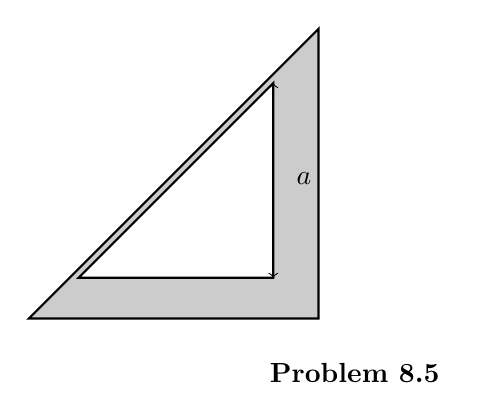
\begin{tikzpicture}[scale=1.15]
  % shaded triangular wall border
  \fill[gray!40] (0,0) -- (3.2,0) -- (3.2,3.2) -- cycle;
  \fill[white] (0.55,0.45) -- (2.7,0.45) -- (2.7,2.6) -- cycle;
  \draw[thick] (0,0) -- (3.2,0) -- (3.2,3.2) -- cycle;
  \draw[thick] (0.55,0.45) -- (2.7,0.45) -- (2.7,2.6) -- cycle;
  % a dimension on right
  \draw[<->] (2.7,2.6) -- (2.7,0.45);
  \node[right] at (2.85,1.55) {$a$};
  \node at (3.6,-0.6) {\textbf{Problem 8.5}};
\end{tikzpicture}
\end{center}

\begin{enumerate}
\item[(b)] For the lowest modes of each type calculate the attenuation constant, assuming that the walls have large, but finite, conductivity. Compare the result with that for a square guide of side $a$ made from the same material.
\end{enumerate}
\solution

Choose the triangle $0<y<x<a$, one half of the square
$0<x,y<a$.  Reflection across $x=y$ converts the triangular
boundary conditions into a parity condition in the square.

\textbf{(a)} TM fields vanish on all three sides.  Antisymmetric
combinations of the square's Dirichlet modes give
\[
E_z=E_0\left[\sin\frac{m\pi x}{a}\sin\frac{n\pi y}{a}
-\sin\frac{n\pi x}{a}\sin\frac{m\pi y}{a}\right],
\quad m>n\geq1.
\]
TE fields have zero normal derivative.  The required symmetric
Neumann combinations are
\[
H_z=H_0\left[\cos\frac{m\pi x}{a}\cos\frac{n\pi y}{a}
+\cos\frac{n\pi x}{a}\cos\frac{m\pi y}{a}\right],
\quad m\geq n\geq0,\quad(m,n)\ne(0,0).
\]
For $m=n$ the redundant factor of two can be absorbed into $H_0$.
Reflection gives a complete set, and for both types
\[
\boxed{\omega_{c,mn}=\frac{\pi c}{a}\sqrt{m^2+n^2},\qquad
k^2=(\omega/c)^2-(\pi/a)^2(m^2+n^2).}
\]
There is no TEM mode in this simply connected hollow cross section.
The lowest TE and TM fields are respectively
$\cos(\pi x/a)+\cos(\pi y/a)$ and the antisymmetric $(2,1)$
combination; their cutoffs are $\pi c/a$ and $\sqrt5\pi c/a$.

\textbf{(b)} Set $R_s=1/(\sigma\delta)$, $\eta_0=\sqrt{\mu_0/\epsilon_0}$,
$t=\omega_c/\omega$ and $s=\sqrt{1-t^2}$ for the mode in question.
For TM modes the general surface-loss expression is
\[
\beta_{\rm TM}=\frac{R_s\omega\epsilon_0}{2k\gamma^2}
\frac{\oint|\partial_n\psi|^2dl}{\int|\psi|^2dA}.
\]
For the lowest TM mode of unit longitudinal amplitude,
$\psi^2$ is symmetric across the diagonal. Orthogonality of the
two sine products over the full square therefore gives
$N=\tfrac12[2(a/2)^2]=a^2/4$. The bottom and right normal
derivatives, up to an irrelevant overall sign, are
\[
\frac{\pi}{a}\left[\sin\frac{2\pi x}{a}-2\sin\frac{\pi x}{a}\right],
\qquad
\frac{\pi}{a}\left[2\sin\frac{\pi y}{a}+\sin\frac{2\pi y}{a}\right].
\]
Their squared integrals are each
$(\pi/a)^2(a/2)(1+4)=5\pi^2/(2a)$. On the diagonal, put
$x=y=u$, use $dl=\sqrt2\,du$, and find
$|\partial_n\psi|^2=(8\pi^2/a^2)\sin^6(\pi u/a)$.
Since $\int_0^\pi\sin^6v\,dv=5\pi/16$, the diagonal contributes
$5\sqrt2\pi^2/(2a)$.  Consequently
\[
\boxed{\beta_{{\rm TM},21}^{\triangle}
=\frac{R_s}{\eta_0a\sqrt{1-(\omega_{c,21}/\omega)^2}}
(2+\sqrt2).}
\]

For the lowest TE field $\psi=\cos(\pi x/a)+\cos(\pi y/a)$,
$\gamma=\pi/a$ and direct integrals on the same three sides give
\[
N=\frac{a^2}2,\qquad S_0=\oint\psi^2dl=a(3+2\sqrt2),\qquad
S_1=\oint|\partial_s\psi|^2dl=\frac{\pi^2}{a}(1+\sqrt2).
\]
For example, the bottom and right contributions to $S_0$ are each
$3a/2$, while the diagonal gives $2\sqrt2a$; their contributions
to $S_1$ are $\pi^2/(2a),\pi^2/(2a),\sqrt2\pi^2/a$.
Use
\[
\beta_{\rm TE}=\frac{R_s\gamma^2}{2\omega\mu_0kN}
\left(S_0+\frac{k^2}{\gamma^4}S_1\right)
\]
to obtain
\[
\boxed{\beta_{{\rm TE},10}^{\triangle}
=\frac{R_s}{\eta_0a s}
\left[(1+\sqrt2)+(2+\sqrt2)t^2\right].}
\]
For comparison, the square of side $a$ has
\[
\beta_{{\rm TE},10}^{\square}=\frac{R_s}{\eta_0a s}(1+2t^2),
\quad\omega_{c,10}^{\square}=\pi c/a,
\qquad
\beta_{{\rm TM},11}^{\square}=\frac{2R_s}{\eta_0a s},
\quad\omega_{c,11}^{\square}=\sqrt2\pi c/a.
\]
The TE cutoffs are the same, so their attenuation ratio at fixed
frequency is $[(1+\sqrt2)+(2+\sqrt2)t^2]/(1+2t^2)$.
For TM the square has the lower cutoff.  At a fixed frequency above
both cutoffs, the ratio is
$(1+1/\sqrt2)s_{\square}/s_{\triangle}$.

\Needspace{5\baselineskip}
\par\bigskip
\noindent\textbf{8.6}\quad A resonant cavity of copper consists of a hollow, right circular cylinder of inner radius $R$ and length $L$, with flat end faces.
\begin{enumerate}
\item[(a)] Determine the resonant frequencies of the cavity for all types of waves. With $(1/\sqrt{\mu\epsilon}\,R)$ as a unit of frequency, plot the lowest four resonant frequencies of each type as a function of $R/L$ for $0<R/L<2$. Does the same mode have the lowest frequency for all $R/L$?
\item[(b)] If $R=2$ cm, $L=3$ cm, and the cavity is made of pure copper, what is the numerical value of $Q$ for the lowest resonant mode?
\end{enumerate}
\solution

\textbf{(a)} Separation in $z$ imposes different axial standing waves:
$E_z=\psi(\rho,\phi)\cos(p\pi z/L)$ for TM, with $p=0,1,\ldots$,
and $H_z=\psi(\rho,\phi)\sin(p\pi z/L)$ for TE, with $p=1,2,\ldots$.
At an end plate the tangential electric field must vanish.
For TM fields it is proportional to $\partial_zE_z$, so a cosine
standing wave satisfies both end conditions. For TE fields it is
proportional to $H_z$, so a sine is required. The TM solution with
$p=0$ remains nonzero; the analogous TE sine would vanish identically.
The side-wall conditions are those of Problem 8.4, so
\[
\boxed{\omega_{mnp}^{\rm TM}=\frac1{\sqrt{\mu\epsilon}R}
\sqrt{x_{mn}^2+(p\pi R/L)^2},\qquad
\omega_{mnp}^{\rm TE}=\frac1{\sqrt{\mu\epsilon}R}
\sqrt{x_{mn}'^{\,2}+(p\pi R/L)^2}.}
\]
Here $m=0,1,\ldots$, $n=1,2,\ldots$ and only positive radial roots
are retained.  Every $m>0$ family has two angular polarizations.
The plots show the four smallest frequencies at each aspect ratio,
counting a polarization pair once.  The ordering can change as
axial and radial families cross, so the plotted curves are the
ordered eigenvalues, not four fixed mode labels.
\begin{center}
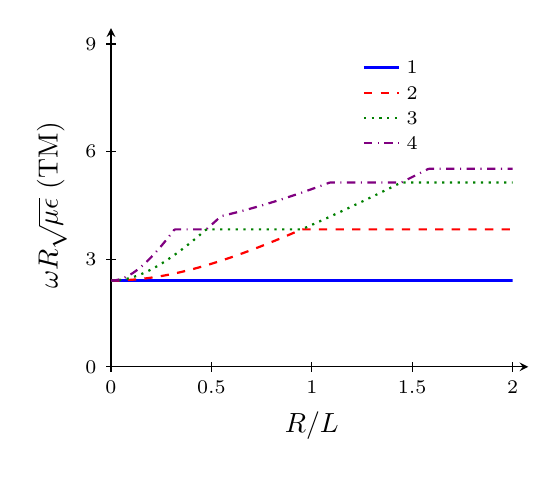
\begin{tikzpicture}[x=1cm,y=1cm,>=stealth]
\draw[->] (0,0)--(5.3,0);
\draw[->] (0,0)--(0,4.3);
\draw (0.00000,.06)--(0.00000,-.06) node[below] {\scriptsize $0$};
\draw (1.27500,.06)--(1.27500,-.06) node[below] {\scriptsize $0.5$};
\draw (2.55000,.06)--(2.55000,-.06) node[below] {\scriptsize $1$};
\draw (3.82500,.06)--(3.82500,-.06) node[below] {\scriptsize $1.5$};
\draw (5.10000,.06)--(5.10000,-.06) node[below] {\scriptsize $2$};
\draw (.06,0.00000)--(-.06,0.00000) node[left] {\scriptsize $0$};
\draw (.06,1.36667)--(-.06,1.36667) node[left] {\scriptsize $3$};
\draw (.06,2.73333)--(-.06,2.73333) node[left] {\scriptsize $6$};
\draw (.06,4.10000)--(-.06,4.10000) node[left] {\scriptsize $9$};
\node[below] at (2.55,-.45) {$R/L$};
\node[rotate=90] at (-.75,2.05) {$\omega R\sqrt{\mu\epsilon}$ (TM)};
\begin{scope}
\clip (0,0) rectangle (5.1,4.1);
\draw[blue,thick] plot coordinates {(0.002550,1.095532) (0.018529,1.095532) (0.034509,1.095532) (0.050488,1.095532) (0.066468,1.095532) (0.082447,1.095532) (0.098427,1.095532) (0.114406,1.095532) (0.130386,1.095532) (0.146365,1.095532) (0.162345,1.095532) (0.178324,1.095532) (0.194304,1.095532) (0.210283,1.095532) (0.226263,1.095532) (0.242242,1.095532) (0.258221,1.095532) (0.274201,1.095532) (0.290180,1.095532) (0.306160,1.095532) (0.322139,1.095532) (0.338119,1.095532) (0.354098,1.095532) (0.370078,1.095532) (0.386057,1.095532) (0.402037,1.095532) (0.418016,1.095532) (0.433996,1.095532) (0.449975,1.095532) (0.465955,1.095532) (0.481934,1.095532) (0.497913,1.095532) (0.513893,1.095532) (0.529872,1.095532) (0.545852,1.095532) (0.561831,1.095532) (0.577811,1.095532) (0.593790,1.095532) (0.609770,1.095532) (0.625749,1.095532) (0.641729,1.095532) (0.657708,1.095532) (0.673688,1.095532) (0.689667,1.095532) (0.705647,1.095532) (0.721626,1.095532) (0.737605,1.095532) (0.753585,1.095532) (0.769564,1.095532) (0.785544,1.095532) (0.801523,1.095532) (0.817503,1.095532) (0.833482,1.095532) (0.849462,1.095532) (0.865441,1.095532) (0.881421,1.095532) (0.897400,1.095532) (0.913380,1.095532) (0.929359,1.095532) (0.945339,1.095532) (0.961318,1.095532) (0.977297,1.095532) (0.993277,1.095532) (1.009256,1.095532) (1.025236,1.095532) (1.041215,1.095532) (1.057195,1.095532) (1.073174,1.095532) (1.089154,1.095532) (1.105133,1.095532) (1.121113,1.095532) (1.137092,1.095532) (1.153072,1.095532) (1.169051,1.095532) (1.185031,1.095532) (1.201010,1.095532) (1.216989,1.095532) (1.232969,1.095532) (1.248948,1.095532) (1.264928,1.095532) (1.280907,1.095532) (1.296887,1.095532) (1.312866,1.095532) (1.328846,1.095532) (1.344825,1.095532) (1.360805,1.095532) (1.376784,1.095532) (1.392764,1.095532) (1.408743,1.095532) (1.424723,1.095532) (1.440702,1.095532) (1.456682,1.095532) (1.472661,1.095532) (1.488640,1.095532) (1.504620,1.095532) (1.520599,1.095532) (1.536579,1.095532) (1.552558,1.095532) (1.568538,1.095532) (1.584517,1.095532) (1.600497,1.095532) (1.616476,1.095532) (1.632456,1.095532) (1.648435,1.095532) (1.664415,1.095532) (1.680394,1.095532) (1.696374,1.095532) (1.712353,1.095532) (1.728332,1.095532) (1.744312,1.095532) (1.760291,1.095532) (1.776271,1.095532) (1.792250,1.095532) (1.808230,1.095532) (1.824209,1.095532) (1.840189,1.095532) (1.856168,1.095532) (1.872148,1.095532) (1.888127,1.095532) (1.904107,1.095532) (1.920086,1.095532) (1.936066,1.095532) (1.952045,1.095532) (1.968024,1.095532) (1.984004,1.095532) (1.999983,1.095532) (2.015963,1.095532) (2.031942,1.095532) (2.047922,1.095532) (2.063901,1.095532) (2.079881,1.095532) (2.095860,1.095532) (2.111840,1.095532) (2.127819,1.095532) (2.143799,1.095532) (2.159778,1.095532) (2.175758,1.095532) (2.191737,1.095532) (2.207716,1.095532) (2.223696,1.095532) (2.239675,1.095532) (2.255655,1.095532) (2.271634,1.095532) (2.287614,1.095532) (2.303593,1.095532) (2.319573,1.095532) (2.335552,1.095532) (2.351532,1.095532) (2.367511,1.095532) (2.383491,1.095532) (2.399470,1.095532) (2.415450,1.095532) (2.431429,1.095532) (2.447408,1.095532) (2.463388,1.095532) (2.479367,1.095532) (2.495347,1.095532) (2.511326,1.095532) (2.527306,1.095532) (2.543285,1.095532) (2.559265,1.095532) (2.575244,1.095532) (2.591224,1.095532) (2.607203,1.095532) (2.623183,1.095532) (2.639162,1.095532) (2.655142,1.095532) (2.671121,1.095532) (2.687100,1.095532) (2.703080,1.095532) (2.719059,1.095532) (2.735039,1.095532) (2.751018,1.095532) (2.766998,1.095532) (2.782977,1.095532) (2.798957,1.095532) (2.814936,1.095532) (2.830916,1.095532) (2.846895,1.095532) (2.862875,1.095532) (2.878854,1.095532) (2.894834,1.095532) (2.910813,1.095532) (2.926792,1.095532) (2.942772,1.095532) (2.958751,1.095532) (2.974731,1.095532) (2.990710,1.095532) (3.006690,1.095532) (3.022669,1.095532) (3.038649,1.095532) (3.054628,1.095532) (3.070608,1.095532) (3.086587,1.095532) (3.102567,1.095532) (3.118546,1.095532) (3.134526,1.095532) (3.150505,1.095532) (3.166484,1.095532) (3.182464,1.095532) (3.198443,1.095532) (3.214423,1.095532) (3.230402,1.095532) (3.246382,1.095532) (3.262361,1.095532) (3.278341,1.095532) (3.294320,1.095532) (3.310300,1.095532) (3.326279,1.095532) (3.342259,1.095532) (3.358238,1.095532) (3.374218,1.095532) (3.390197,1.095532) (3.406176,1.095532) (3.422156,1.095532) (3.438135,1.095532) (3.454115,1.095532) (3.470094,1.095532) (3.486074,1.095532) (3.502053,1.095532) (3.518033,1.095532) (3.534012,1.095532) (3.549992,1.095532) (3.565971,1.095532) (3.581951,1.095532) (3.597930,1.095532) (3.613910,1.095532) (3.629889,1.095532) (3.645868,1.095532) (3.661848,1.095532) (3.677827,1.095532) (3.693807,1.095532) (3.709786,1.095532) (3.725766,1.095532) (3.741745,1.095532) (3.757725,1.095532) (3.773704,1.095532) (3.789684,1.095532) (3.805663,1.095532) (3.821643,1.095532) (3.837622,1.095532) (3.853602,1.095532) (3.869581,1.095532) (3.885561,1.095532) (3.901540,1.095532) (3.917519,1.095532) (3.933499,1.095532) (3.949478,1.095532) (3.965458,1.095532) (3.981437,1.095532) (3.997417,1.095532) (4.013396,1.095532) (4.029376,1.095532) (4.045355,1.095532) (4.061335,1.095532) (4.077314,1.095532) (4.093294,1.095532) (4.109273,1.095532) (4.125253,1.095532) (4.141232,1.095532) (4.157211,1.095532) (4.173191,1.095532) (4.189170,1.095532) (4.205150,1.095532) (4.221129,1.095532) (4.237109,1.095532) (4.253088,1.095532) (4.269068,1.095532) (4.285047,1.095532) (4.301027,1.095532) (4.317006,1.095532) (4.332986,1.095532) (4.348965,1.095532) (4.364945,1.095532) (4.380924,1.095532) (4.396903,1.095532) (4.412883,1.095532) (4.428862,1.095532) (4.444842,1.095532) (4.460821,1.095532) (4.476801,1.095532) (4.492780,1.095532) (4.508760,1.095532) (4.524739,1.095532) (4.540719,1.095532) (4.556698,1.095532) (4.572678,1.095532) (4.588657,1.095532) (4.604637,1.095532) (4.620616,1.095532) (4.636595,1.095532) (4.652575,1.095532) (4.668554,1.095532) (4.684534,1.095532) (4.700513,1.095532) (4.716493,1.095532) (4.732472,1.095532) (4.748452,1.095532) (4.764431,1.095532) (4.780411,1.095532) (4.796390,1.095532) (4.812370,1.095532) (4.828349,1.095532) (4.844329,1.095532) (4.860308,1.095532) (4.876287,1.095532) (4.892267,1.095532) (4.908246,1.095532) (4.924226,1.095532) (4.940205,1.095532) (4.956185,1.095532) (4.972164,1.095532) (4.988144,1.095532) (5.004123,1.095532) (5.020103,1.095532) (5.036082,1.095532) (5.052062,1.095532) (5.068041,1.095532) (5.084021,1.095532) (5.100000,1.095532)};
\draw[red,dashed,thick] plot coordinates {(0.002550,1.095533) (0.018529,1.095581) (0.034509,1.095703) (0.050488,1.095898) (0.066468,1.096167) (0.082447,1.096508) (0.098427,1.096924) (0.114406,1.097412) (0.130386,1.097973) (0.146365,1.098607) (0.162345,1.099314) (0.178324,1.100094) (0.194304,1.100946) (0.210283,1.101870) (0.226263,1.102867) (0.242242,1.103936) (0.258221,1.105076) (0.274201,1.106288) (0.290180,1.107571) (0.306160,1.108925) (0.322139,1.110350) (0.338119,1.111846) (0.354098,1.113412) (0.370078,1.115047) (0.386057,1.116753) (0.402037,1.118527) (0.418016,1.120371) (0.433996,1.122283) (0.449975,1.124264) (0.465955,1.126312) (0.481934,1.128428) (0.497913,1.130611) (0.513893,1.132861) (0.529872,1.135178) (0.545852,1.137560) (0.561831,1.140008) (0.577811,1.142521) (0.593790,1.145099) (0.609770,1.147741) (0.625749,1.150447) (0.641729,1.153217) (0.657708,1.156049) (0.673688,1.158944) (0.689667,1.161901) (0.705647,1.164919) (0.721626,1.167999) (0.737605,1.171139) (0.753585,1.174339) (0.769564,1.177598) (0.785544,1.180917) (0.801523,1.184295) (0.817503,1.187730) (0.833482,1.191224) (0.849462,1.194774) (0.865441,1.198381) (0.881421,1.202044) (0.897400,1.205762) (0.913380,1.209536) (0.929359,1.213364) (0.945339,1.217246) (0.961318,1.221182) (0.977297,1.225171) (0.993277,1.229212) (1.009256,1.233305) (1.025236,1.237450) (1.041215,1.241646) (1.057195,1.245892) (1.073174,1.250188) (1.089154,1.254533) (1.105133,1.258927) (1.121113,1.263370) (1.137092,1.267860) (1.153072,1.272398) (1.169051,1.276983) (1.185031,1.281614) (1.201010,1.286291) (1.216989,1.291013) (1.232969,1.295781) (1.248948,1.300592) (1.264928,1.305447) (1.280907,1.310346) (1.296887,1.315288) (1.312866,1.320272) (1.328846,1.325298) (1.344825,1.330366) (1.360805,1.335474) (1.376784,1.340623) (1.392764,1.345813) (1.408743,1.351041) (1.424723,1.356309) (1.440702,1.361616) (1.456682,1.366961) (1.472661,1.372343) (1.488640,1.377763) (1.504620,1.383220) (1.520599,1.388714) (1.536579,1.394243) (1.552558,1.399808) (1.568538,1.405408) (1.584517,1.411043) (1.600497,1.416713) (1.616476,1.422416) (1.632456,1.428153) (1.648435,1.433923) (1.664415,1.439725) (1.680394,1.445561) (1.696374,1.451428) (1.712353,1.457326) (1.728332,1.463256) (1.744312,1.469217) (1.760291,1.475208) (1.776271,1.481229) (1.792250,1.487280) (1.808230,1.493360) (1.824209,1.499469) (1.840189,1.505607) (1.856168,1.511773) (1.872148,1.517967) (1.888127,1.524188) (1.904107,1.530437) (1.920086,1.536713) (1.936066,1.543015) (1.952045,1.549344) (1.968024,1.555699) (1.984004,1.562079) (1.999983,1.568485) (2.015963,1.574915) (2.031942,1.581371) (2.047922,1.587850) (2.063901,1.594354) (2.079881,1.600882) (2.095860,1.607433) (2.111840,1.614007) (2.127819,1.620605) (2.143799,1.627225) (2.159778,1.633867) (2.175758,1.640532) (2.191737,1.647219) (2.207716,1.653927) (2.223696,1.660656) (2.239675,1.667407) (2.255655,1.674178) (2.271634,1.680970) (2.287614,1.687782) (2.303593,1.694614) (2.319573,1.701466) (2.335552,1.708338) (2.351532,1.715229) (2.367511,1.722139) (2.383491,1.729069) (2.399470,1.736016) (2.415450,1.742983) (2.431429,1.745555) (2.447408,1.745555) (2.463388,1.745555) (2.479367,1.745555) (2.495347,1.745555) (2.511326,1.745555) (2.527306,1.745555) (2.543285,1.745555) (2.559265,1.745555) (2.575244,1.745555) (2.591224,1.745555) (2.607203,1.745555) (2.623183,1.745555) (2.639162,1.745555) (2.655142,1.745555) (2.671121,1.745555) (2.687100,1.745555) (2.703080,1.745555) (2.719059,1.745555) (2.735039,1.745555) (2.751018,1.745555) (2.766998,1.745555) (2.782977,1.745555) (2.798957,1.745555) (2.814936,1.745555) (2.830916,1.745555) (2.846895,1.745555) (2.862875,1.745555) (2.878854,1.745555) (2.894834,1.745555) (2.910813,1.745555) (2.926792,1.745555) (2.942772,1.745555) (2.958751,1.745555) (2.974731,1.745555) (2.990710,1.745555) (3.006690,1.745555) (3.022669,1.745555) (3.038649,1.745555) (3.054628,1.745555) (3.070608,1.745555) (3.086587,1.745555) (3.102567,1.745555) (3.118546,1.745555) (3.134526,1.745555) (3.150505,1.745555) (3.166484,1.745555) (3.182464,1.745555) (3.198443,1.745555) (3.214423,1.745555) (3.230402,1.745555) (3.246382,1.745555) (3.262361,1.745555) (3.278341,1.745555) (3.294320,1.745555) (3.310300,1.745555) (3.326279,1.745555) (3.342259,1.745555) (3.358238,1.745555) (3.374218,1.745555) (3.390197,1.745555) (3.406176,1.745555) (3.422156,1.745555) (3.438135,1.745555) (3.454115,1.745555) (3.470094,1.745555) (3.486074,1.745555) (3.502053,1.745555) (3.518033,1.745555) (3.534012,1.745555) (3.549992,1.745555) (3.565971,1.745555) (3.581951,1.745555) (3.597930,1.745555) (3.613910,1.745555) (3.629889,1.745555) (3.645868,1.745555) (3.661848,1.745555) (3.677827,1.745555) (3.693807,1.745555) (3.709786,1.745555) (3.725766,1.745555) (3.741745,1.745555) (3.757725,1.745555) (3.773704,1.745555) (3.789684,1.745555) (3.805663,1.745555) (3.821643,1.745555) (3.837622,1.745555) (3.853602,1.745555) (3.869581,1.745555) (3.885561,1.745555) (3.901540,1.745555) (3.917519,1.745555) (3.933499,1.745555) (3.949478,1.745555) (3.965458,1.745555) (3.981437,1.745555) (3.997417,1.745555) (4.013396,1.745555) (4.029376,1.745555) (4.045355,1.745555) (4.061335,1.745555) (4.077314,1.745555) (4.093294,1.745555) (4.109273,1.745555) (4.125253,1.745555) (4.141232,1.745555) (4.157211,1.745555) (4.173191,1.745555) (4.189170,1.745555) (4.205150,1.745555) (4.221129,1.745555) (4.237109,1.745555) (4.253088,1.745555) (4.269068,1.745555) (4.285047,1.745555) (4.301027,1.745555) (4.317006,1.745555) (4.332986,1.745555) (4.348965,1.745555) (4.364945,1.745555) (4.380924,1.745555) (4.396903,1.745555) (4.412883,1.745555) (4.428862,1.745555) (4.444842,1.745555) (4.460821,1.745555) (4.476801,1.745555) (4.492780,1.745555) (4.508760,1.745555) (4.524739,1.745555) (4.540719,1.745555) (4.556698,1.745555) (4.572678,1.745555) (4.588657,1.745555) (4.604637,1.745555) (4.620616,1.745555) (4.636595,1.745555) (4.652575,1.745555) (4.668554,1.745555) (4.684534,1.745555) (4.700513,1.745555) (4.716493,1.745555) (4.732472,1.745555) (4.748452,1.745555) (4.764431,1.745555) (4.780411,1.745555) (4.796390,1.745555) (4.812370,1.745555) (4.828349,1.745555) (4.844329,1.745555) (4.860308,1.745555) (4.876287,1.745555) (4.892267,1.745555) (4.908246,1.745555) (4.924226,1.745555) (4.940205,1.745555) (4.956185,1.745555) (4.972164,1.745555) (4.988144,1.745555) (5.004123,1.745555) (5.020103,1.745555) (5.036082,1.745555) (5.052062,1.745555) (5.068041,1.745555) (5.084021,1.745555) (5.100000,1.745555)};
\draw[green!50!black,dotted,thick] plot coordinates {(0.002550,1.095535) (0.018529,1.095729) (0.034509,1.096216) (0.050488,1.096997) (0.066468,1.098069) (0.082447,1.099434) (0.098427,1.101089) (0.114406,1.103033) (0.130386,1.105265) (0.146365,1.107782) (0.162345,1.110584) (0.178324,1.113668) (0.194304,1.117031) (0.210283,1.120671) (0.226263,1.124586) (0.242242,1.128772) (0.258221,1.133227) (0.274201,1.137947) (0.290180,1.142928) (0.306160,1.148169) (0.322139,1.153665) (0.338119,1.159412) (0.354098,1.165407) (0.370078,1.171645) (0.386057,1.178124) (0.402037,1.184839) (0.418016,1.191786) (0.433996,1.198962) (0.449975,1.206361) (0.465955,1.213980) (0.481934,1.221815) (0.497913,1.229862) (0.513893,1.238116) (0.529872,1.246574) (0.545852,1.255231) (0.561831,1.264083) (0.577811,1.273127) (0.593790,1.282357) (0.609770,1.291771) (0.625749,1.301364) (0.641729,1.311132) (0.657708,1.321071) (0.673688,1.331178) (0.689667,1.341449) (0.705647,1.351879) (0.721626,1.362466) (0.737605,1.373206) (0.753585,1.384094) (0.769564,1.395129) (0.785544,1.406305) (0.801523,1.417620) (0.817503,1.429071) (0.833482,1.440654) (0.849462,1.452367) (0.865441,1.464205) (0.881421,1.476167) (0.897400,1.488248) (0.913380,1.500446) (0.929359,1.512759) (0.945339,1.525184) (0.961318,1.537717) (0.977297,1.550356) (0.993277,1.563100) (1.009256,1.575944) (1.025236,1.588887) (1.041215,1.601926) (1.057195,1.615059) (1.073174,1.628283) (1.089154,1.641598) (1.105133,1.654999) (1.121113,1.668486) (1.137092,1.682056) (1.153072,1.695706) (1.169051,1.709437) (1.185031,1.723244) (1.201010,1.737127) (1.216989,1.745555) (1.232969,1.745555) (1.248948,1.745555) (1.264928,1.745555) (1.280907,1.745555) (1.296887,1.745555) (1.312866,1.745555) (1.328846,1.745555) (1.344825,1.745555) (1.360805,1.745555) (1.376784,1.745555) (1.392764,1.745555) (1.408743,1.745555) (1.424723,1.745555) (1.440702,1.745555) (1.456682,1.745555) (1.472661,1.745555) (1.488640,1.745555) (1.504620,1.745555) (1.520599,1.745555) (1.536579,1.745555) (1.552558,1.745555) (1.568538,1.745555) (1.584517,1.745555) (1.600497,1.745555) (1.616476,1.745555) (1.632456,1.745555) (1.648435,1.745555) (1.664415,1.745555) (1.680394,1.745555) (1.696374,1.745555) (1.712353,1.745555) (1.728332,1.745555) (1.744312,1.745555) (1.760291,1.745555) (1.776271,1.745555) (1.792250,1.745555) (1.808230,1.745555) (1.824209,1.745555) (1.840189,1.745555) (1.856168,1.745555) (1.872148,1.745555) (1.888127,1.745555) (1.904107,1.745555) (1.920086,1.745555) (1.936066,1.745555) (1.952045,1.745555) (1.968024,1.745555) (1.984004,1.745555) (1.999983,1.745555) (2.015963,1.745555) (2.031942,1.745555) (2.047922,1.745555) (2.063901,1.745555) (2.079881,1.745555) (2.095860,1.745555) (2.111840,1.745555) (2.127819,1.745555) (2.143799,1.745555) (2.159778,1.745555) (2.175758,1.745555) (2.191737,1.745555) (2.207716,1.745555) (2.223696,1.745555) (2.239675,1.745555) (2.255655,1.745555) (2.271634,1.745555) (2.287614,1.745555) (2.303593,1.745555) (2.319573,1.745555) (2.335552,1.745555) (2.351532,1.745555) (2.367511,1.745555) (2.383491,1.745555) (2.399470,1.745555) (2.415450,1.745555) (2.431429,1.749967) (2.447408,1.756970) (2.463388,1.763990) (2.479367,1.771028) (2.495347,1.778083) (2.511326,1.785156) (2.527306,1.792245) (2.543285,1.799351) (2.559265,1.806474) (2.575244,1.813613) (2.591224,1.820768) (2.607203,1.827940) (2.623183,1.835127) (2.639162,1.842329) (2.655142,1.849547) (2.671121,1.856781) (2.687100,1.864029) (2.703080,1.871293) (2.719059,1.878571) (2.735039,1.885864) (2.751018,1.893171) (2.766998,1.900492) (2.782977,1.907827) (2.798957,1.915177) (2.814936,1.922540) (2.830916,1.929916) (2.846895,1.937306) (2.862875,1.944710) (2.878854,1.952126) (2.894834,1.959555) (2.910813,1.966998) (2.926792,1.974453) (2.942772,1.981920) (2.958751,1.989400) (2.974731,1.996892) (2.990710,2.004396) (3.006690,2.011912) (3.022669,2.019441) (3.038649,2.026980) (3.054628,2.034532) (3.070608,2.042095) (3.086587,2.049669) (3.102567,2.057254) (3.118546,2.064851) (3.134526,2.072458) (3.150505,2.080077) (3.166484,2.087706) (3.182464,2.095345) (3.198443,2.102995) (3.214423,2.110656) (3.230402,2.118327) (3.246382,2.126008) (3.262361,2.133699) (3.278341,2.141399) (3.294320,2.149110) (3.310300,2.156831) (3.326279,2.164561) (3.342259,2.172300) (3.358238,2.180049) (3.374218,2.187808) (3.390197,2.195575) (3.406176,2.203352) (3.422156,2.211138) (3.438135,2.218932) (3.454115,2.226736) (3.470094,2.234548) (3.486074,2.242369) (3.502053,2.250198) (3.518033,2.258036) (3.534012,2.265883) (3.549992,2.273737) (3.565971,2.281600) (3.581951,2.289471) (3.597930,2.297350) (3.613910,2.305237) (3.629889,2.313132) (3.645868,2.321034) (3.661848,2.328945) (3.677827,2.336863) (3.693807,2.339561) (3.709786,2.339561) (3.725766,2.339561) (3.741745,2.339561) (3.757725,2.339561) (3.773704,2.339561) (3.789684,2.339561) (3.805663,2.339561) (3.821643,2.339561) (3.837622,2.339561) (3.853602,2.339561) (3.869581,2.339561) (3.885561,2.339561) (3.901540,2.339561) (3.917519,2.339561) (3.933499,2.339561) (3.949478,2.339561) (3.965458,2.339561) (3.981437,2.339561) (3.997417,2.339561) (4.013396,2.339561) (4.029376,2.339561) (4.045355,2.339561) (4.061335,2.339561) (4.077314,2.339561) (4.093294,2.339561) (4.109273,2.339561) (4.125253,2.339561) (4.141232,2.339561) (4.157211,2.339561) (4.173191,2.339561) (4.189170,2.339561) (4.205150,2.339561) (4.221129,2.339561) (4.237109,2.339561) (4.253088,2.339561) (4.269068,2.339561) (4.285047,2.339561) (4.301027,2.339561) (4.317006,2.339561) (4.332986,2.339561) (4.348965,2.339561) (4.364945,2.339561) (4.380924,2.339561) (4.396903,2.339561) (4.412883,2.339561) (4.428862,2.339561) (4.444842,2.339561) (4.460821,2.339561) (4.476801,2.339561) (4.492780,2.339561) (4.508760,2.339561) (4.524739,2.339561) (4.540719,2.339561) (4.556698,2.339561) (4.572678,2.339561) (4.588657,2.339561) (4.604637,2.339561) (4.620616,2.339561) (4.636595,2.339561) (4.652575,2.339561) (4.668554,2.339561) (4.684534,2.339561) (4.700513,2.339561) (4.716493,2.339561) (4.732472,2.339561) (4.748452,2.339561) (4.764431,2.339561) (4.780411,2.339561) (4.796390,2.339561) (4.812370,2.339561) (4.828349,2.339561) (4.844329,2.339561) (4.860308,2.339561) (4.876287,2.339561) (4.892267,2.339561) (4.908246,2.339561) (4.924226,2.339561) (4.940205,2.339561) (4.956185,2.339561) (4.972164,2.339561) (4.988144,2.339561) (5.004123,2.339561) (5.020103,2.339561) (5.036082,2.339561) (5.052062,2.339561) (5.068041,2.339561) (5.084021,2.339561) (5.100000,2.339561)};
\draw[violet,dash dot,thick] plot coordinates {(0.002550,1.095540) (0.018529,1.095976) (0.034509,1.097071) (0.050488,1.098825) (0.066468,1.101233) (0.082447,1.104292) (0.098427,1.107996) (0.114406,1.112338) (0.130386,1.117311) (0.146365,1.122908) (0.162345,1.129118) (0.178324,1.135931) (0.194304,1.143337) (0.210283,1.151324) (0.226263,1.159881) (0.242242,1.168994) (0.258221,1.178651) (0.274201,1.188839) (0.290180,1.199544) (0.306160,1.210752) (0.322139,1.222449) (0.338119,1.234623) (0.354098,1.247257) (0.370078,1.260340) (0.386057,1.273856) (0.402037,1.287793) (0.418016,1.302137) (0.433996,1.316874) (0.449975,1.331992) (0.465955,1.347477) (0.481934,1.363318) (0.497913,1.379501) (0.513893,1.396015) (0.529872,1.412849) (0.545852,1.429991) (0.561831,1.447430) (0.577811,1.465155) (0.593790,1.483157) (0.609770,1.501425) (0.625749,1.519949) (0.641729,1.538722) (0.657708,1.557732) (0.673688,1.576973) (0.689667,1.596435) (0.705647,1.616111) (0.721626,1.635992) (0.737605,1.656072) (0.753585,1.676343) (0.769564,1.696799) (0.785544,1.717433) (0.801523,1.738238) (0.817503,1.745555) (0.833482,1.745555) (0.849462,1.745555) (0.865441,1.745555) (0.881421,1.745555) (0.897400,1.745555) (0.913380,1.745555) (0.929359,1.745555) (0.945339,1.745555) (0.961318,1.745555) (0.977297,1.745555) (0.993277,1.745555) (1.009256,1.745555) (1.025236,1.745555) (1.041215,1.745555) (1.057195,1.745555) (1.073174,1.745555) (1.089154,1.745555) (1.105133,1.745555) (1.121113,1.745555) (1.137092,1.745555) (1.153072,1.745555) (1.169051,1.745555) (1.185031,1.745555) (1.201010,1.745555) (1.216989,1.751083) (1.232969,1.765112) (1.248948,1.779211) (1.264928,1.793378) (1.280907,1.807612) (1.296887,1.821912) (1.312866,1.836275) (1.328846,1.850701) (1.344825,1.865187) (1.360805,1.879734) (1.376784,1.894338) (1.392764,1.908999) (1.408743,1.916269) (1.424723,1.919986) (1.440702,1.923739) (1.456682,1.927525) (1.472661,1.931346) (1.488640,1.935201) (1.504620,1.939090) (1.520599,1.943013) (1.536579,1.946968) (1.552558,1.950957) (1.568538,1.954979) (1.584517,1.959034) (1.600497,1.963122) (1.616476,1.967242) (1.632456,1.971394) (1.648435,1.975578) (1.664415,1.979793) (1.680394,1.984041) (1.696374,1.988320) (1.712353,1.992629) (1.728332,1.996970) (1.744312,2.001342) (1.760291,2.005744) (1.776271,2.010177) (1.792250,2.014640) (1.808230,2.019132) (1.824209,2.023655) (1.840189,2.028207) (1.856168,2.032789) (1.872148,2.037399) (1.888127,2.042039) (1.904107,2.046707) (1.920086,2.051404) (1.936066,2.056130) (1.952045,2.060883) (1.968024,2.065665) (1.984004,2.070474) (1.999983,2.075311) (2.015963,2.080176) (2.031942,2.085067) (2.047922,2.089986) (2.063901,2.094931) (2.079881,2.099904) (2.095860,2.104902) (2.111840,2.109927) (2.127819,2.114978) (2.143799,2.120055) (2.159778,2.125158) (2.175758,2.130286) (2.191737,2.135439) (2.207716,2.140618) (2.223696,2.145822) (2.239675,2.151050) (2.255655,2.156303) (2.271634,2.161581) (2.287614,2.166883) (2.303593,2.172209) (2.319573,2.177558) (2.335552,2.182932) (2.351532,2.188329) (2.367511,2.193750) (2.383491,2.199193) (2.399470,2.204660) (2.415450,2.210150) (2.431429,2.215662) (2.447408,2.221197) (2.463388,2.226754) (2.479367,2.232333) (2.495347,2.237935) (2.511326,2.243558) (2.527306,2.249203) (2.543285,2.254870) (2.559265,2.260557) (2.575244,2.266267) (2.591224,2.271997) (2.607203,2.277748) (2.623183,2.283520) (2.639162,2.289312) (2.655142,2.295125) (2.671121,2.300958) (2.687100,2.306811) (2.703080,2.312684) (2.719059,2.318577) (2.735039,2.324490) (2.751018,2.330422) (2.766998,2.336374) (2.782977,2.339561) (2.798957,2.339561) (2.814936,2.339561) (2.830916,2.339561) (2.846895,2.339561) (2.862875,2.339561) (2.878854,2.339561) (2.894834,2.339561) (2.910813,2.339561) (2.926792,2.339561) (2.942772,2.339561) (2.958751,2.339561) (2.974731,2.339561) (2.990710,2.339561) (3.006690,2.339561) (3.022669,2.339561) (3.038649,2.339561) (3.054628,2.339561) (3.070608,2.339561) (3.086587,2.339561) (3.102567,2.339561) (3.118546,2.339561) (3.134526,2.339561) (3.150505,2.339561) (3.166484,2.339561) (3.182464,2.339561) (3.198443,2.339561) (3.214423,2.339561) (3.230402,2.339561) (3.246382,2.339561) (3.262361,2.339561) (3.278341,2.339561) (3.294320,2.339561) (3.310300,2.339561) (3.326279,2.339561) (3.342259,2.339561) (3.358238,2.339561) (3.374218,2.339561) (3.390197,2.339561) (3.406176,2.339561) (3.422156,2.339561) (3.438135,2.339561) (3.454115,2.339561) (3.470094,2.339561) (3.486074,2.339561) (3.502053,2.339561) (3.518033,2.339561) (3.534012,2.339561) (3.549992,2.339561) (3.565971,2.339561) (3.581951,2.339561) (3.597930,2.339561) (3.613910,2.339561) (3.629889,2.339561) (3.645868,2.339561) (3.661848,2.339561) (3.677827,2.339561) (3.693807,2.344788) (3.709786,2.352721) (3.725766,2.360662) (3.741745,2.368609) (3.757725,2.376565) (3.773704,2.384527) (3.789684,2.392496) (3.805663,2.400473) (3.821643,2.408456) (3.837622,2.416446) (3.853602,2.424443) (3.869581,2.432447) (3.885561,2.440458) (3.901540,2.448475) (3.917519,2.456499) (3.933499,2.464529) (3.949478,2.472566) (3.965458,2.480609) (3.981437,2.488659) (3.997417,2.496715) (4.013396,2.504777) (4.029376,2.512845) (4.045355,2.514702) (4.061335,2.514702) (4.077314,2.514702) (4.093294,2.514702) (4.109273,2.514702) (4.125253,2.514702) (4.141232,2.514702) (4.157211,2.514702) (4.173191,2.514702) (4.189170,2.514702) (4.205150,2.514702) (4.221129,2.514702) (4.237109,2.514702) (4.253088,2.514702) (4.269068,2.514702) (4.285047,2.514702) (4.301027,2.514702) (4.317006,2.514702) (4.332986,2.514702) (4.348965,2.514702) (4.364945,2.514702) (4.380924,2.514702) (4.396903,2.514702) (4.412883,2.514702) (4.428862,2.514702) (4.444842,2.514702) (4.460821,2.514702) (4.476801,2.514702) (4.492780,2.514702) (4.508760,2.514702) (4.524739,2.514702) (4.540719,2.514702) (4.556698,2.514702) (4.572678,2.514702) (4.588657,2.514702) (4.604637,2.514702) (4.620616,2.514702) (4.636595,2.514702) (4.652575,2.514702) (4.668554,2.514702) (4.684534,2.514702) (4.700513,2.514702) (4.716493,2.514702) (4.732472,2.514702) (4.748452,2.514702) (4.764431,2.514702) (4.780411,2.514702) (4.796390,2.514702) (4.812370,2.514702) (4.828349,2.514702) (4.844329,2.514702) (4.860308,2.514702) (4.876287,2.514702) (4.892267,2.514702) (4.908246,2.514702) (4.924226,2.514702) (4.940205,2.514702) (4.956185,2.514702) (4.972164,2.514702) (4.988144,2.514702) (5.004123,2.514702) (5.020103,2.514702) (5.036082,2.514702) (5.052062,2.514702) (5.068041,2.514702) (5.084021,2.514702) (5.100000,2.514702)};
\end{scope}
\draw[blue,thick] (3.2129999999999996,3.8)--(3.663,3.8);
\node[right,fill=white,inner sep=1pt] at (3.7129999999999996,3.8) {\scriptsize 1};
\draw[red,dashed,thick] (3.2129999999999996,3.48)--(3.663,3.48);
\node[right,fill=white,inner sep=1pt] at (3.7129999999999996,3.48) {\scriptsize 2};
\draw[green!50!black,dotted,thick] (3.2129999999999996,3.1599999999999997)--(3.663,3.1599999999999997);
\node[right,fill=white,inner sep=1pt] at (3.7129999999999996,3.1599999999999997) {\scriptsize 3};
\draw[violet,dash dot,thick] (3.2129999999999996,2.84)--(3.663,2.84);
\node[right,fill=white,inner sep=1pt] at (3.7129999999999996,2.84) {\scriptsize 4};
\end{tikzpicture}
\quad
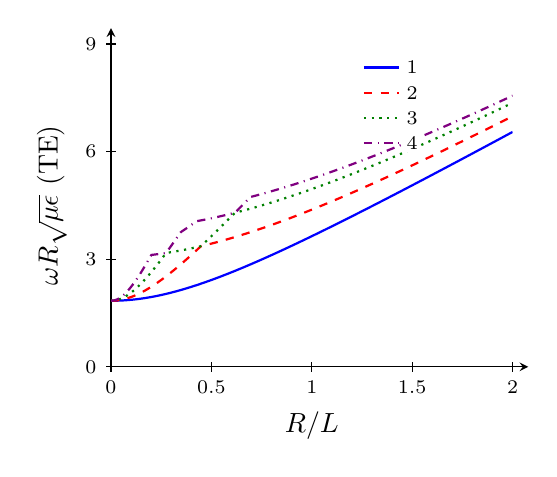
\begin{tikzpicture}[x=1cm,y=1cm,>=stealth]
\draw[->] (0,0)--(5.3,0);
\draw[->] (0,0)--(0,4.3);
\draw (0.00000,.06)--(0.00000,-.06) node[below] {\scriptsize $0$};
\draw (1.27500,.06)--(1.27500,-.06) node[below] {\scriptsize $0.5$};
\draw (2.55000,.06)--(2.55000,-.06) node[below] {\scriptsize $1$};
\draw (3.82500,.06)--(3.82500,-.06) node[below] {\scriptsize $1.5$};
\draw (5.10000,.06)--(5.10000,-.06) node[below] {\scriptsize $2$};
\draw (.06,0.00000)--(-.06,0.00000) node[left] {\scriptsize $0$};
\draw (.06,1.36667)--(-.06,1.36667) node[left] {\scriptsize $3$};
\draw (.06,2.73333)--(-.06,2.73333) node[left] {\scriptsize $6$};
\draw (.06,4.10000)--(-.06,4.10000) node[left] {\scriptsize $9$};
\node[below] at (2.55,-.45) {$R/L$};
\node[rotate=90] at (-.75,2.05) {$\omega R\sqrt{\mu\epsilon}$ (TE)};
\begin{scope}
\clip (0,0) rectangle (5.1,4.1);
\draw[blue,thick] plot coordinates {(0.002550,0.838763) (0.018529,0.838826) (0.034509,0.838985) (0.050488,0.839240) (0.066468,0.839591) (0.082447,0.840037) (0.098427,0.840579) (0.114406,0.841216) (0.130386,0.841948) (0.146365,0.842775) (0.162345,0.843696) (0.178324,0.844711) (0.194304,0.845821) (0.210283,0.847024) (0.226263,0.848320) (0.242242,0.849709) (0.258221,0.851190) (0.274201,0.852763) (0.290180,0.854427) (0.306160,0.856181) (0.322139,0.858026) (0.338119,0.859961) (0.354098,0.861984) (0.370078,0.864096) (0.386057,0.866295) (0.402037,0.868582) (0.418016,0.870955) (0.433996,0.873413) (0.449975,0.875957) (0.465955,0.878584) (0.481934,0.881295) (0.497913,0.884089) (0.513893,0.886965) (0.529872,0.889921) (0.545852,0.892958) (0.561831,0.896075) (0.577811,0.899270) (0.593790,0.902543) (0.609770,0.905893) (0.625749,0.909319) (0.641729,0.912820) (0.657708,0.916396) (0.673688,0.920045) (0.689667,0.923767) (0.705647,0.927560) (0.721626,0.931425) (0.737605,0.935359) (0.753585,0.939363) (0.769564,0.943435) (0.785544,0.947574) (0.801523,0.951780) (0.817503,0.956052) (0.833482,0.960388) (0.849462,0.964788) (0.865441,0.969251) (0.881421,0.973776) (0.897400,0.978363) (0.913380,0.983010) (0.929359,0.987716) (0.945339,0.992482) (0.961318,0.997305) (0.977297,1.002185) (0.993277,1.007121) (1.009256,1.012113) (1.025236,1.017160) (1.041215,1.022260) (1.057195,1.027413) (1.073174,1.032618) (1.089154,1.037875) (1.105133,1.043182) (1.121113,1.048539) (1.137092,1.053946) (1.153072,1.059400) (1.169051,1.064902) (1.185031,1.070451) (1.201010,1.076046) (1.216989,1.081687) (1.232969,1.087372) (1.248948,1.093102) (1.264928,1.098874) (1.280907,1.104689) (1.296887,1.110547) (1.312866,1.116445) (1.328846,1.122384) (1.344825,1.128364) (1.360805,1.134382) (1.376784,1.140440) (1.392764,1.146535) (1.408743,1.152668) (1.424723,1.158838) (1.440702,1.165045) (1.456682,1.171287) (1.472661,1.177564) (1.488640,1.183876) (1.504620,1.190222) (1.520599,1.196602) (1.536579,1.203015) (1.552558,1.209460) (1.568538,1.215937) (1.584517,1.222446) (1.600497,1.228986) (1.616476,1.235556) (1.632456,1.242156) (1.648435,1.248786) (1.664415,1.255444) (1.680394,1.262132) (1.696374,1.268847) (1.712353,1.275590) (1.728332,1.282361) (1.744312,1.289158) (1.760291,1.295982) (1.776271,1.302832) (1.792250,1.309707) (1.808230,1.316607) (1.824209,1.323533) (1.840189,1.330482) (1.856168,1.337456) (1.872148,1.344453) (1.888127,1.351474) (1.904107,1.358517) (1.920086,1.365583) (1.936066,1.372672) (1.952045,1.379782) (1.968024,1.386914) (1.984004,1.394067) (1.999983,1.401241) (2.015963,1.408435) (2.031942,1.415650) (2.047922,1.422884) (2.063901,1.430139) (2.079881,1.437412) (2.095860,1.444705) (2.111840,1.452016) (2.127819,1.459346) (2.143799,1.466694) (2.159778,1.474060) (2.175758,1.481444) (2.191737,1.488845) (2.207716,1.496264) (2.223696,1.503699) (2.239675,1.511151) (2.255655,1.518619) (2.271634,1.526103) (2.287614,1.533603) (2.303593,1.541119) (2.319573,1.548651) (2.335552,1.556197) (2.351532,1.563759) (2.367511,1.571336) (2.383491,1.578927) (2.399470,1.586532) (2.415450,1.594152) (2.431429,1.601785) (2.447408,1.609433) (2.463388,1.617094) (2.479367,1.624768) (2.495347,1.632455) (2.511326,1.640156) (2.527306,1.647869) (2.543285,1.655595) (2.559265,1.663334) (2.575244,1.671084) (2.591224,1.678847) (2.607203,1.686622) (2.623183,1.694409) (2.639162,1.702207) (2.655142,1.710017) (2.671121,1.717838) (2.687100,1.725670) (2.703080,1.733513) (2.719059,1.741367) (2.735039,1.749232) (2.751018,1.757107) (2.766998,1.764993) (2.782977,1.772889) (2.798957,1.780796) (2.814936,1.788712) (2.830916,1.796638) (2.846895,1.804574) (2.862875,1.812519) (2.878854,1.820474) (2.894834,1.828439) (2.910813,1.836413) (2.926792,1.844395) (2.942772,1.852387) (2.958751,1.860388) (2.974731,1.868397) (2.990710,1.876416) (3.006690,1.884442) (3.022669,1.892478) (3.038649,1.900521) (3.054628,1.908573) (3.070608,1.916633) (3.086587,1.924701) (3.102567,1.932777) (3.118546,1.940861) (3.134526,1.948952) (3.150505,1.957051) (3.166484,1.965158) (3.182464,1.973272) (3.198443,1.981394) (3.214423,1.989522) (3.230402,1.997658) (3.246382,2.005801) (3.262361,2.013952) (3.278341,2.022109) (3.294320,2.030272) (3.310300,2.038443) (3.326279,2.046620) (3.342259,2.054804) (3.358238,2.062995) (3.374218,2.071192) (3.390197,2.079395) (3.406176,2.087604) (3.422156,2.095820) (3.438135,2.104042) (3.454115,2.112270) (3.470094,2.120504) (3.486074,2.128744) (3.502053,2.136990) (3.518033,2.145241) (3.534012,2.153498) (3.549992,2.161761) (3.565971,2.170030) (3.581951,2.178304) (3.597930,2.186584) (3.613910,2.194869) (3.629889,2.203159) (3.645868,2.211455) (3.661848,2.219756) (3.677827,2.228062) (3.693807,2.236373) (3.709786,2.244689) (3.725766,2.253010) (3.741745,2.261336) (3.757725,2.269667) (3.773704,2.278003) (3.789684,2.286344) (3.805663,2.294689) (3.821643,2.303040) (3.837622,2.311394) (3.853602,2.319754) (3.869581,2.328117) (3.885561,2.336486) (3.901540,2.344859) (3.917519,2.353236) (3.933499,2.361617) (3.949478,2.370003) (3.965458,2.378393) (3.981437,2.386787) (3.997417,2.395186) (4.013396,2.403588) (4.029376,2.411995) (4.045355,2.420406) (4.061335,2.428820) (4.077314,2.437239) (4.093294,2.445661) (4.109273,2.454088) (4.125253,2.462518) (4.141232,2.470952) (4.157211,2.479390) (4.173191,2.487831) (4.189170,2.496276) (4.205150,2.504725) (4.221129,2.513177) (4.237109,2.521633) (4.253088,2.530093) (4.269068,2.538556) (4.285047,2.547022) (4.301027,2.555492) (4.317006,2.563965) (4.332986,2.572442) (4.348965,2.580922) (4.364945,2.589405) (4.380924,2.597891) (4.396903,2.606381) (4.412883,2.614874) (4.428862,2.623370) (4.444842,2.631869) (4.460821,2.640371) (4.476801,2.648877) (4.492780,2.657385) (4.508760,2.665896) (4.524739,2.674411) (4.540719,2.682928) (4.556698,2.691448) (4.572678,2.699972) (4.588657,2.708498) (4.604637,2.717027) (4.620616,2.725558) (4.636595,2.734093) (4.652575,2.742630) (4.668554,2.751170) (4.684534,2.759713) (4.700513,2.768258) (4.716493,2.776807) (4.732472,2.785357) (4.748452,2.793911) (4.764431,2.802467) (4.780411,2.811025) (4.796390,2.819586) (4.812370,2.828150) (4.828349,2.836716) (4.844329,2.845285) (4.860308,2.853856) (4.876287,2.862429) (4.892267,2.871005) (4.908246,2.879583) (4.924226,2.888164) (4.940205,2.896747) (4.956185,2.905332) (4.972164,2.913920) (4.988144,2.922510) (5.004123,2.931102) (5.020103,2.939697) (5.036082,2.948293) (5.052062,2.956892) (5.068041,2.965493) (5.084021,2.974097) (5.100000,2.982702)};
\draw[red,dashed,thick] plot coordinates {(0.002550,0.838766) (0.018529,0.839019) (0.034509,0.839655) (0.050488,0.840674) (0.066468,0.842073) (0.082447,0.843852) (0.098427,0.846007) (0.114406,0.848535) (0.130386,0.851435) (0.146365,0.854701) (0.162345,0.858329) (0.178324,0.862315) (0.194304,0.866654) (0.210283,0.871341) (0.226263,0.876370) (0.242242,0.881736) (0.258221,0.887431) (0.274201,0.893450) (0.290180,0.899787) (0.306160,0.906434) (0.322139,0.913386) (0.338119,0.920634) (0.354098,0.928172) (0.370078,0.935994) (0.386057,0.944091) (0.402037,0.952457) (0.418016,0.961086) (0.433996,0.969969) (0.449975,0.979100) (0.465955,0.988473) (0.481934,0.998080) (0.497913,1.007914) (0.513893,1.017970) (0.529872,1.028240) (0.545852,1.038718) (0.561831,1.049399) (0.577811,1.060275) (0.593790,1.071341) (0.609770,1.082591) (0.625749,1.094020) (0.641729,1.105621) (0.657708,1.117390) (0.673688,1.129321) (0.689667,1.141410) (0.705647,1.153650) (0.721626,1.166038) (0.737605,1.178569) (0.753585,1.191238) (0.769564,1.204041) (0.785544,1.216974) (0.801523,1.230032) (0.817503,1.243212) (0.833482,1.256510) (0.849462,1.269921) (0.865441,1.283444) (0.881421,1.297073) (0.897400,1.310806) (0.913380,1.324640) (0.929359,1.338571) (0.945339,1.352596) (0.961318,1.366713) (0.977297,1.380919) (0.993277,1.395210) (1.009256,1.409585) (1.025236,1.424041) (1.041215,1.438575) (1.057195,1.453185) (1.073174,1.467869) (1.089154,1.482624) (1.105133,1.497449) (1.121113,1.512341) (1.137092,1.527299) (1.153072,1.534513) (1.169051,1.538317) (1.185031,1.542164) (1.201010,1.546052) (1.216989,1.549984) (1.232969,1.553957) (1.248948,1.557971) (1.264928,1.562027) (1.280907,1.566123) (1.296887,1.570260) (1.312866,1.574437) (1.328846,1.578654) (1.344825,1.582911) (1.360805,1.587207) (1.376784,1.591542) (1.392764,1.595915) (1.408743,1.600327) (1.424723,1.604777) (1.440702,1.609264) (1.456682,1.613789) (1.472661,1.618351) (1.488640,1.622950) (1.504620,1.627585) (1.520599,1.632256) (1.536579,1.636963) (1.552558,1.641705) (1.568538,1.646483) (1.584517,1.651295) (1.600497,1.656143) (1.616476,1.661024) (1.632456,1.665939) (1.648435,1.670888) (1.664415,1.675871) (1.680394,1.680886) (1.696374,1.685935) (1.712353,1.691015) (1.728332,1.696128) (1.744312,1.701273) (1.760291,1.706450) (1.776271,1.711658) (1.792250,1.716897) (1.808230,1.722166) (1.824209,1.727467) (1.840189,1.732797) (1.856168,1.738157) (1.872148,1.743547) (1.888127,1.748967) (1.904107,1.754415) (1.920086,1.759892) (1.936066,1.765398) (1.952045,1.770932) (1.968024,1.776494) (1.984004,1.782084) (1.999983,1.787702) (2.015963,1.793347) (2.031942,1.799018) (2.047922,1.804717) (2.063901,1.810442) (2.079881,1.816193) (2.095860,1.821970) (2.111840,1.827773) (2.127819,1.833601) (2.143799,1.839455) (2.159778,1.845334) (2.175758,1.851237) (2.191737,1.857165) (2.207716,1.863118) (2.223696,1.869094) (2.239675,1.875094) (2.255655,1.881118) (2.271634,1.887165) (2.287614,1.893236) (2.303593,1.899329) (2.319573,1.905445) (2.335552,1.911584) (2.351532,1.917745) (2.367511,1.923928) (2.383491,1.930133) (2.399470,1.936359) (2.415450,1.942607) (2.431429,1.948876) (2.447408,1.955166) (2.463388,1.961478) (2.479367,1.967809) (2.495347,1.974161) (2.511326,1.980534) (2.527306,1.986926) (2.543285,1.993338) (2.559265,1.999770) (2.575244,2.006222) (2.591224,2.012692) (2.607203,2.019182) (2.623183,2.025691) (2.639162,2.032218) (2.655142,2.038764) (2.671121,2.045329) (2.687100,2.051911) (2.703080,2.058512) (2.719059,2.065130) (2.735039,2.071766) (2.751018,2.078420) (2.766998,2.085091) (2.782977,2.091779) (2.798957,2.098484) (2.814936,2.105206) (2.830916,2.111945) (2.846895,2.118700) (2.862875,2.125471) (2.878854,2.132259) (2.894834,2.139063) (2.910813,2.145883) (2.926792,2.152718) (2.942772,2.159570) (2.958751,2.166436) (2.974731,2.173318) (2.990710,2.180215) (3.006690,2.187127) (3.022669,2.194054) (3.038649,2.200996) (3.054628,2.207952) (3.070608,2.214923) (3.086587,2.221908) (3.102567,2.228908) (3.118546,2.235921) (3.134526,2.242948) (3.150505,2.249989) (3.166484,2.257044) (3.182464,2.264112) (3.198443,2.271194) (3.214423,2.278289) (3.230402,2.285397) (3.246382,2.292519) (3.262361,2.299653) (3.278341,2.306800) (3.294320,2.313959) (3.310300,2.321132) (3.326279,2.328316) (3.342259,2.335513) (3.358238,2.342723) (3.374218,2.349944) (3.390197,2.357177) (3.406176,2.364423) (3.422156,2.371680) (3.438135,2.378948) (3.454115,2.386229) (3.470094,2.393520) (3.486074,2.400823) (3.502053,2.408138) (3.518033,2.415463) (3.534012,2.422800) (3.549992,2.430147) (3.565971,2.437505) (3.581951,2.444874) (3.597930,2.452254) (3.613910,2.459644) (3.629889,2.467045) (3.645868,2.474456) (3.661848,2.481878) (3.677827,2.489309) (3.693807,2.496751) (3.709786,2.504203) (3.725766,2.511664) (3.741745,2.519136) (3.757725,2.526617) (3.773704,2.534108) (3.789684,2.541608) (3.805663,2.549118) (3.821643,2.556637) (3.837622,2.564166) (3.853602,2.571704) (3.869581,2.579251) (3.885561,2.586807) (3.901540,2.594372) (3.917519,2.601946) (3.933499,2.609528) (3.949478,2.617120) (3.965458,2.624720) (3.981437,2.632329) (3.997417,2.639946) (4.013396,2.647572) (4.029376,2.655207) (4.045355,2.662849) (4.061335,2.670500) (4.077314,2.678159) (4.093294,2.685826) (4.109273,2.693501) (4.125253,2.701184) (4.141232,2.708875) (4.157211,2.716574) (4.173191,2.724281) (4.189170,2.731995) (4.205150,2.739717) (4.221129,2.747447) (4.237109,2.755184) (4.253088,2.762928) (4.269068,2.770680) (4.285047,2.778439) (4.301027,2.786205) (4.317006,2.793979) (4.332986,2.801760) (4.348965,2.809548) (4.364945,2.817343) (4.380924,2.825144) (4.396903,2.832953) (4.412883,2.840769) (4.428862,2.848591) (4.444842,2.856420) (4.460821,2.864256) (4.476801,2.872099) (4.492780,2.879948) (4.508760,2.887803) (4.524739,2.895665) (4.540719,2.903533) (4.556698,2.911408) (4.572678,2.919289) (4.588657,2.927177) (4.604637,2.935070) (4.620616,2.942970) (4.636595,2.950876) (4.652575,2.958787) (4.668554,2.966705) (4.684534,2.974629) (4.700513,2.982559) (4.716493,2.990495) (4.732472,2.998436) (4.748452,3.006383) (4.764431,3.014336) (4.780411,3.022295) (4.796390,3.030259) (4.812370,3.038229) (4.828349,3.046204) (4.844329,3.054185) (4.860308,3.062172) (4.876287,3.070163) (4.892267,3.078161) (4.908246,3.086163) (4.924226,3.094171) (4.940205,3.102184) (4.956185,3.110202) (4.972164,3.118226) (4.988144,3.126255) (5.004123,3.134288) (5.020103,3.142327) (5.036082,3.150371) (5.052062,3.158420) (5.068041,3.166473) (5.084021,3.174532) (5.100000,3.182595)};
\draw[green!50!black,dotted,thick] plot coordinates {(0.002550,0.838772) (0.018529,0.839342) (0.034509,0.840772) (0.050488,0.843058) (0.066468,0.846195) (0.082447,0.850171) (0.098427,0.854977) (0.114406,0.860597) (0.130386,0.867016) (0.146365,0.874216) (0.162345,0.882178) (0.178324,0.890882) (0.194304,0.900306) (0.210283,0.910428) (0.226263,0.921225) (0.242242,0.932673) (0.258221,0.944749) (0.274201,0.957429) (0.290180,0.970689) (0.306160,0.984506) (0.322139,0.998856) (0.338119,1.013718) (0.354098,1.029069) (0.370078,1.044887) (0.386057,1.061151) (0.402037,1.077842) (0.418016,1.094939) (0.433996,1.112425) (0.449975,1.130280) (0.465955,1.148489) (0.481934,1.167033) (0.497913,1.185898) (0.513893,1.205068) (0.529872,1.224530) (0.545852,1.244269) (0.561831,1.264272) (0.577811,1.284527) (0.593790,1.305023) (0.609770,1.325748) (0.625749,1.346691) (0.641729,1.367843) (0.657708,1.389194) (0.673688,1.410736) (0.689667,1.432458) (0.705647,1.446641) (0.721626,1.449122) (0.737605,1.451654) (0.753585,1.454237) (0.769564,1.456871) (0.785544,1.459555) (0.801523,1.462289) (0.817503,1.465072) (0.833482,1.467906) (0.849462,1.470788) (0.865441,1.473720) (0.881421,1.476700) (0.897400,1.479728) (0.913380,1.482805) (0.929359,1.485929) (0.945339,1.489101) (0.961318,1.492320) (0.977297,1.495586) (0.993277,1.498898) (1.009256,1.502257) (1.025236,1.505661) (1.041215,1.509111) (1.057195,1.512607) (1.073174,1.516147) (1.089154,1.519732) (1.105133,1.523362) (1.121113,1.527035) (1.137092,1.530753) (1.153072,1.542320) (1.169051,1.557403) (1.185031,1.572546) (1.201010,1.587747) (1.216989,1.603005) (1.232969,1.618317) (1.248948,1.633683) (1.264928,1.649101) (1.280907,1.664570) (1.296887,1.680087) (1.312866,1.695652) (1.328846,1.711264) (1.344825,1.726921) (1.360805,1.742622) (1.376784,1.758365) (1.392764,1.774150) (1.408743,1.789976) (1.424723,1.805841) (1.440702,1.821745) (1.456682,1.837686) (1.472661,1.853663) (1.488640,1.869676) (1.504620,1.885724) (1.520599,1.901806) (1.536579,1.917920) (1.552558,1.934066) (1.568538,1.950244) (1.584517,1.959034) (1.600497,1.963122) (1.616476,1.967242) (1.632456,1.971394) (1.648435,1.975578) (1.664415,1.979793) (1.680394,1.984041) (1.696374,1.988320) (1.712353,1.992629) (1.728332,1.996970) (1.744312,2.001342) (1.760291,2.005744) (1.776271,2.010177) (1.792250,2.014640) (1.808230,2.019132) (1.824209,2.023655) (1.840189,2.028207) (1.856168,2.032789) (1.872148,2.037399) (1.888127,2.042039) (1.904107,2.046707) (1.920086,2.051404) (1.936066,2.056130) (1.952045,2.060883) (1.968024,2.065665) (1.984004,2.070474) (1.999983,2.075311) (2.015963,2.080176) (2.031942,2.085067) (2.047922,2.089986) (2.063901,2.094931) (2.079881,2.099904) (2.095860,2.104902) (2.111840,2.109927) (2.127819,2.114978) (2.143799,2.120055) (2.159778,2.125158) (2.175758,2.130286) (2.191737,2.135439) (2.207716,2.140618) (2.223696,2.145822) (2.239675,2.151050) (2.255655,2.156303) (2.271634,2.161581) (2.287614,2.166883) (2.303593,2.172209) (2.319573,2.177558) (2.335552,2.182932) (2.351532,2.188329) (2.367511,2.193750) (2.383491,2.199193) (2.399470,2.204660) (2.415450,2.210150) (2.431429,2.215662) (2.447408,2.221197) (2.463388,2.226754) (2.479367,2.232333) (2.495347,2.237935) (2.511326,2.243558) (2.527306,2.249203) (2.543285,2.254870) (2.559265,2.260557) (2.575244,2.266267) (2.591224,2.271997) (2.607203,2.277748) (2.623183,2.283520) (2.639162,2.289312) (2.655142,2.295125) (2.671121,2.300958) (2.687100,2.306811) (2.703080,2.312684) (2.719059,2.318577) (2.735039,2.324490) (2.751018,2.330422) (2.766998,2.336374) (2.782977,2.342344) (2.798957,2.348334) (2.814936,2.354343) (2.830916,2.360371) (2.846895,2.366417) (2.862875,2.372481) (2.878854,2.378564) (2.894834,2.384666) (2.910813,2.390785) (2.926792,2.396922) (2.942772,2.403077) (2.958751,2.409250) (2.974731,2.415440) (2.990710,2.421648) (3.006690,2.427872) (3.022669,2.434114) (3.038649,2.440373) (3.054628,2.446649) (3.070608,2.452942) (3.086587,2.459251) (3.102567,2.465577) (3.118546,2.471919) (3.134526,2.478277) (3.150505,2.484651) (3.166484,2.491041) (3.182464,2.497447) (3.198443,2.503869) (3.214423,2.510307) (3.230402,2.516760) (3.246382,2.523228) (3.262361,2.529712) (3.278341,2.536211) (3.294320,2.542724) (3.310300,2.549253) (3.326279,2.555797) (3.342259,2.562355) (3.358238,2.568927) (3.374218,2.575515) (3.390197,2.582116) (3.406176,2.588732) (3.422156,2.595362) (3.438135,2.602006) (3.454115,2.608664) (3.470094,2.615335) (3.486074,2.622020) (3.502053,2.628719) (3.518033,2.635432) (3.534012,2.642158) (3.549992,2.648897) (3.565971,2.655649) (3.581951,2.662414) (3.597930,2.669193) (3.613910,2.675984) (3.629889,2.682788) (3.645868,2.689605) (3.661848,2.696434) (3.677827,2.703276) (3.693807,2.710130) (3.709786,2.716996) (3.725766,2.723875) (3.741745,2.730766) (3.757725,2.737669) (3.773704,2.744584) (3.789684,2.751511) (3.805663,2.758449) (3.821643,2.765399) (3.837622,2.772361) (3.853602,2.779334) (3.869581,2.786319) (3.885561,2.793315) (3.901540,2.800322) (3.917519,2.807340) (3.933499,2.814370) (3.949478,2.821410) (3.965458,2.828462) (3.981437,2.835524) (3.997417,2.842597) (4.013396,2.849680) (4.029376,2.856775) (4.045355,2.863879) (4.061335,2.870994) (4.077314,2.878120) (4.093294,2.885256) (4.109273,2.892402) (4.125253,2.899558) (4.141232,2.906724) (4.157211,2.913900) (4.173191,2.921086) (4.189170,2.928282) (4.205150,2.935488) (4.221129,2.942703) (4.237109,2.949928) (4.253088,2.957163) (4.269068,2.964406) (4.285047,2.971660) (4.301027,2.978923) (4.317006,2.986195) (4.332986,2.993476) (4.348965,3.000766) (4.364945,3.008066) (4.380924,3.015374) (4.396903,3.022691) (4.412883,3.030018) (4.428862,3.037353) (4.444842,3.044696) (4.460821,3.052049) (4.476801,3.059410) (4.492780,3.066779) (4.508760,3.074158) (4.524739,3.081544) (4.540719,3.088939) (4.556698,3.096342) (4.572678,3.103754) (4.588657,3.111174) (4.604637,3.118601) (4.620616,3.126037) (4.636595,3.133481) (4.652575,3.140933) (4.668554,3.148393) (4.684534,3.155861) (4.700513,3.163336) (4.716493,3.170819) (4.732472,3.178310) (4.748452,3.185809) (4.764431,3.193315) (4.780411,3.200829) (4.796390,3.208350) (4.812370,3.215878) (4.828349,3.223414) (4.844329,3.230957) (4.860308,3.238508) (4.876287,3.246066) (4.892267,3.253631) (4.908246,3.261203) (4.924226,3.268782) (4.940205,3.276368) (4.956185,3.283961) (4.972164,3.291561) (4.988144,3.299167) (5.004123,3.306781) (5.020103,3.314402) (5.036082,3.322029) (5.052062,3.329663) (5.068041,3.337303) (5.084021,3.344950) (5.100000,3.352604)};
\draw[violet,dash dot,thick] plot coordinates {(0.002550,0.838781) (0.018529,0.839792) (0.034509,0.842332) (0.050488,0.846385) (0.066468,0.851931) (0.082447,0.858941) (0.098427,0.867379) (0.114406,0.877204) (0.130386,0.888370) (0.146365,0.900827) (0.162345,0.914523) (0.178324,0.929402) (0.194304,0.945408) (0.210283,0.962486) (0.226263,0.980580) (0.242242,0.999634) (0.258221,1.019595) (0.274201,1.040409) (0.290180,1.062028) (0.306160,1.084403) (0.322139,1.107488) (0.338119,1.131240) (0.354098,1.155618) (0.370078,1.180582) (0.386057,1.206096) (0.402037,1.232127) (0.418016,1.258642) (0.433996,1.285612) (0.449975,1.313007) (0.465955,1.340803) (0.481934,1.368974) (0.497913,1.397499) (0.513893,1.420953) (0.529872,1.422801) (0.545852,1.424702) (0.561831,1.426658) (0.577811,1.428667) (0.593790,1.430729) (0.609770,1.432845) (0.625749,1.435013) (0.641729,1.437234) (0.657708,1.439508) (0.673688,1.441834) (0.689667,1.444212) (0.705647,1.454354) (0.721626,1.476415) (0.737605,1.498635) (0.753585,1.521006) (0.769564,1.543521) (0.785544,1.566176) (0.801523,1.588963) (0.817503,1.611876) (0.833482,1.634912) (0.849462,1.658064) (0.865441,1.681327) (0.881421,1.704698) (0.897400,1.717736) (0.913380,1.728315) (0.929359,1.739015) (0.945339,1.749834) (0.961318,1.760769) (0.977297,1.771818) (0.993277,1.782979) (1.009256,1.794250) (1.025236,1.805629) (1.041215,1.817113) (1.057195,1.828701) (1.073174,1.840391) (1.089154,1.849493) (1.105133,1.852477) (1.121113,1.855499) (1.137092,1.858559) (1.153072,1.861658) (1.169051,1.864794) (1.185031,1.867969) (1.201010,1.871181) (1.216989,1.874430) (1.232969,1.877717) (1.248948,1.881040) (1.264928,1.884401) (1.280907,1.887798) (1.296887,1.891231) (1.312866,1.894701) (1.328846,1.898207) (1.344825,1.901748) (1.360805,1.905325) (1.376784,1.908938) (1.392764,1.912586) (1.408743,1.916269) (1.424723,1.919986) (1.440702,1.923739) (1.456682,1.927525) (1.472661,1.931346) (1.488640,1.935201) (1.504620,1.939090) (1.520599,1.943013) (1.536579,1.946968) (1.552558,1.950957) (1.568538,1.954979) (1.584517,1.966452) (1.600497,1.982690) (1.616476,1.998957) (1.632456,2.015253) (1.648435,2.031576) (1.664415,2.047926) (1.680394,2.064302) (1.696374,2.080704) (1.712353,2.097132) (1.728332,2.113583) (1.744312,2.130059) (1.760291,2.146558) (1.776271,2.157954) (1.792250,2.162112) (1.808230,2.166299) (1.824209,2.170515) (1.840189,2.174760) (1.856168,2.179033) (1.872148,2.183335) (1.888127,2.187665) (1.904107,2.192023) (1.920086,2.196410) (1.936066,2.200824) (1.952045,2.205265) (1.968024,2.209734) (1.984004,2.214231) (1.999983,2.218755) (2.015963,2.223305) (2.031942,2.227883) (2.047922,2.232487) (2.063901,2.237117) (2.079881,2.241774) (2.095860,2.246457) (2.111840,2.251166) (2.127819,2.255901) (2.143799,2.260661) (2.159778,2.265447) (2.175758,2.270258) (2.191737,2.275095) (2.207716,2.279956) (2.223696,2.284843) (2.239675,2.289754) (2.255655,2.294689) (2.271634,2.299649) (2.287614,2.304634) (2.303593,2.309642) (2.319573,2.314674) (2.335552,2.319730) (2.351532,2.324810) (2.367511,2.329912) (2.383491,2.335039) (2.399470,2.340188) (2.415450,2.345361) (2.431429,2.350556) (2.447408,2.355774) (2.463388,2.361014) (2.479367,2.366277) (2.495347,2.371562) (2.511326,2.376869) (2.527306,2.382198) (2.543285,2.387549) (2.559265,2.392922) (2.575244,2.398316) (2.591224,2.403731) (2.607203,2.409168) (2.623183,2.414626) (2.639162,2.420104) (2.655142,2.425604) (2.671121,2.431124) (2.687100,2.436664) (2.703080,2.442225) (2.719059,2.447806) (2.735039,2.453408) (2.751018,2.459029) (2.766998,2.464670) (2.782977,2.470331) (2.798957,2.476011) (2.814936,2.481710) (2.830916,2.487429) (2.846895,2.493167) (2.862875,2.498924) (2.878854,2.504700) (2.894834,2.510495) (2.910813,2.516308) (2.926792,2.522140) (2.942772,2.527990) (2.958751,2.533859) (2.974731,2.539745) (2.990710,2.545650) (3.006690,2.551572) (3.022669,2.557512) (3.038649,2.563470) (3.054628,2.569445) (3.070608,2.575438) (3.086587,2.581447) (3.102567,2.587474) (3.118546,2.593518) (3.134526,2.599579) (3.150505,2.605657) (3.166484,2.611751) (3.182464,2.617862) (3.198443,2.623989) (3.214423,2.630132) (3.230402,2.636292) (3.246382,2.642468) (3.262361,2.648660) (3.278341,2.654867) (3.294320,2.661090) (3.310300,2.667329) (3.326279,2.673584) (3.342259,2.679854) (3.358238,2.686139) (3.374218,2.692440) (3.390197,2.698755) (3.406176,2.705086) (3.422156,2.711431) (3.438135,2.717791) (3.454115,2.724166) (3.470094,2.730555) (3.486074,2.736959) (3.502053,2.743378) (3.518033,2.749810) (3.534012,2.756257) (3.549992,2.762718) (3.565971,2.769192) (3.581951,2.775681) (3.597930,2.782183) (3.613910,2.788700) (3.629889,2.795229) (3.645868,2.801772) (3.661848,2.808329) (3.677827,2.814899) (3.693807,2.821482) (3.709786,2.828078) (3.725766,2.834687) (3.741745,2.841309) (3.757725,2.847944) (3.773704,2.854592) (3.789684,2.861252) (3.805663,2.867925) (3.821643,2.874611) (3.837622,2.881309) (3.853602,2.888019) (3.869581,2.894741) (3.885561,2.901476) (3.901540,2.908223) (3.917519,2.914981) (3.933499,2.921752) (3.949478,2.928534) (3.965458,2.935328) (3.981437,2.942134) (3.997417,2.948951) (4.013396,2.955780) (4.029376,2.962620) (4.045355,2.969471) (4.061335,2.976334) (4.077314,2.983208) (4.093294,2.990093) (4.109273,2.996989) (4.125253,3.003896) (4.141232,3.010814) (4.157211,3.017742) (4.173191,3.024682) (4.189170,3.031632) (4.205150,3.038592) (4.221129,3.045563) (4.237109,3.052545) (4.253088,3.059537) (4.269068,3.066539) (4.285047,3.073551) (4.301027,3.080574) (4.317006,3.087606) (4.332986,3.094649) (4.348965,3.101702) (4.364945,3.108764) (4.380924,3.115836) (4.396903,3.122918) (4.412883,3.130010) (4.428862,3.137111) (4.444842,3.144222) (4.460821,3.151342) (4.476801,3.158472) (4.492780,3.165611) (4.508760,3.172759) (4.524739,3.179917) (4.540719,3.187083) (4.556698,3.194259) (4.572678,3.201444) (4.588657,3.208638) (4.604637,3.215841) (4.620616,3.223052) (4.636595,3.230273) (4.652575,3.237502) (4.668554,3.244740) (4.684534,3.251986) (4.700513,3.259241) (4.716493,3.266504) (4.732472,3.273776) (4.748452,3.281057) (4.764431,3.288346) (4.780411,3.295643) (4.796390,3.302948) (4.812370,3.310261) (4.828349,3.317583) (4.844329,3.324912) (4.860308,3.332250) (4.876287,3.339595) (4.892267,3.346949) (4.908246,3.354310) (4.924226,3.361679) (4.940205,3.369056) (4.956185,3.376441) (4.972164,3.383833) (4.988144,3.391233) (5.004123,3.398640) (5.020103,3.406055) (5.036082,3.413478) (5.052062,3.420908) (5.068041,3.428345) (5.084021,3.435789) (5.100000,3.443241)};
\end{scope}
\draw[blue,thick] (3.2129999999999996,3.8)--(3.663,3.8);
\node[right,fill=white,inner sep=1pt] at (3.7129999999999996,3.8) {\scriptsize 1};
\draw[red,dashed,thick] (3.2129999999999996,3.48)--(3.663,3.48);
\node[right,fill=white,inner sep=1pt] at (3.7129999999999996,3.48) {\scriptsize 2};
\draw[green!50!black,dotted,thick] (3.2129999999999996,3.1599999999999997)--(3.663,3.1599999999999997);
\node[right,fill=white,inner sep=1pt] at (3.7129999999999996,3.1599999999999997) {\scriptsize 3};
\draw[violet,dash dot,thick] (3.2129999999999996,2.84)--(3.663,2.84);
\node[right,fill=white,inner sep=1pt] at (3.7129999999999996,2.84) {\scriptsize 4};
\end{tikzpicture}

\end{center}
The lowest TM frequency is always $\mathrm{TM}_{010}$,
$\omega R\sqrt{\mu\epsilon}=2.404825558$; the lowest TE frequency
is always $\mathrm{TE}_{111}$,
$\sqrt{1.841183781^2+\pi^2(R/L)^2}$.
Their crossing occurs at
\[
\frac RL=\frac{\sqrt{2.404825558^2-1.841183781^2}}\pi
=0.492427374.
\]
Thus a long cavity has $\mathrm{TE}_{111}$ as its lowest mode,
whereas a shorter cavity has $\mathrm{TM}_{010}$.

\textbf{(b)} For $R/L=2/3$ the lowest mode is $\mathrm{TM}_{010}$.
Write $x=x_{01}$ and $H_\phi=H_1J_1(x\rho/R)$; the fields are
independent of $z$.  At resonance the average electric and magnetic
energies are equal, so
\[
Q=\frac{\omega U}{P_{\ell}}
=\frac{\omega\mu\int_V|H|^2dV}{R_s\oint_S|H_\parallel|^2dS}.
\]
The radial Bessel integral, using $J_0(x)=0$, is
$\int_0^R\rho J_1^2(x\rho/R)d\rho=R^2J_1^2(x)/2$.
Indeed, $J_1'=J_0-J_1/x$ gives $J_1'(x)=-J_1(x)/x$ at this
root; inserting it into the Bessel norm identity derived in
Problem 8.4 cancels the two terms proportional to $J_1^2/x^2$.
Consequently the volume integral is
$\pi R^2L|H_1|^2J_1^2(x)$, while the side wall and the two end
plates contribute respectively
$2\pi RL|H_1|^2J_1^2(x)$ and
$2\pi R^2|H_1|^2J_1^2(x)$.  Therefore
\[
\boxed{Q=\frac{\omega\mu}{R_s}\frac{RL}{2(R+L)}
=\frac\mu{\mu_c}\frac{RL}{\delta(R+L)}.}
\]
For the numerical estimate take vacuum inside, $\mu_c=\mu_0$,
and room-temperature copper represented by
$\sigma=5.80\times10^7\ {\rm S\,m^{-1}}$ (100\% IACS at
$20^\circ$C, NBS \emph{Copper Wire Tables}, Circular 31,
2nd ed., 1914, p.~9).  With $R=0.020$ m and $L=0.030$ m,
\[
\omega=3.60474\times10^{10}\ \mathrm{s^{-1}},\quad
f=5.73713\ \mathrm{GHz},\quad\delta=8.72487\times10^{-7}\ \mathrm{m},
\quad\boxed{Q\simeq1.38\times10^4.}
\]
The material estimate is explicit: $Q=1.37538\times10^4
\sqrt{\sigma/(5.80\times10^7\ {\rm S\,m^{-1}})}$ under these
geometric and permeability assumptions.  A more precise value for
``pure copper'' requires its temperature and conductivity.

\Needspace{5\baselineskip}
\par\bigskip
\noindent\textbf{8.7}\quad A resonant cavity consists of the empty space between two perfectly conducting, concentric spherical shells, the smaller having an outer radius $a$ and the larger an inner radius $b$. As shown in Section 8.9, the azimuthal magnetic field has a radial dependence given by spherical Bessel functions, $j_{l}(kr)$ and $n_{l}(kr)$, where $k=\omega/c$.
\begin{enumerate}
\item[(a)] Write down the transcendental equation for the characteristic frequencies of the cavity for arbitrary $l$.
\item[(b)] For $l=1$ use the explicit forms of the spherical Bessel functions to show that the characteristic frequencies are given by
\[
\frac{\tan kh}{kh}=\frac{\left(k^{2}+\dfrac{1}{ab}\right)}{k^{2}+ab\left(k^{2}-\dfrac{1}{a^{2}}\right)\!\left(k^{2}-\dfrac{1}{b^{2}}\right)}
\]
where $h=b-a$.
\item[(c)] For $h/a\ll1$, verify that the result of part b yields the frequency found in Section 8.9, and find the first order correction in $h/a$. [The result of part b seems to have been derived first by J.~J. Thomson and published in his book \emph{Recent Researches in Electricity and Magnetism}, Oxford Clarendon Press, 1893, pp.~373 ff.]
\end{enumerate}
\solution

\textbf{(a)} For the electric-multipole (TM) family used in
Section 8.9, put
$u_l(r)=r[A j_l(kr)+B n_l(kr)]$.  The radial equation and the
conducting boundary conditions are
\[
u_l''+\left[k^2-\frac{l(l+1)}{r^2}\right]u_l=0,\qquad
u_l'(a)=u_l'(b)=0.
\]
The tangential electric field is proportional to $u_l'$.  Eliminating
$A,B$ gives
\[
\boxed{[j_l(ka)+ka j_l'(ka)][n_l(kb)+kb n_l'(kb)]
-[n_l(ka)+ka n_l'(ka)][j_l(kb)+kb j_l'(kb)]=0.}
\]
Take $l\geq1$ and nonzero $k$; the $2l+1$ azimuthal orientations
are degenerate.  For completeness the cavity also has a
magnetic-multipole (TE) family, whose tangential electric field
vanishes when $u_l(a)=u_l(b)=0$.  Its equation is
$j_l(ka)n_l(kb)-n_l(ka)j_l(kb)=0$.
Parts (b)--(c) concern the first, Schumann-resonance family.

\textbf{(b)} For $l=1$,
\[
j_1(x)=\frac{\sin x}{x^2}-\frac{\cos x}{x},\qquad
n_1(x)=-\frac{\cos x}{x^2}-\frac{\sin x}{x}.
\]
Define $A_r=k^2-r^{-2}$ and $B_r=k/r$.  Direct differentiation gives
\[
\frac d{dr}[rj_1(kr)]=k^{-2}[A_r\sin(kr)+B_r\cos(kr)],\quad
\frac d{dr}[rn_1(kr)]=k^{-2}[-A_r\cos(kr)+B_r\sin(kr)].
\]
Their determinant reduces by angle-subtraction identities to
\[
(A_aA_b+B_aB_b)\sin(kh)+(A_aB_b-B_aA_b)\cos(kh)=0.
\]
Now
\[
A_aB_b-B_aA_b=-\frac{kh}{ab}\left(k^2+\frac1{ab}\right),\quad
ab(A_aA_b+B_aB_b)=k^2+ab(k^2-a^{-2})(k^2-b^{-2}).
\]
Division gives exactly the stated formula for $\tan(kh)/(kh)$.
At poles or zeros of quantities used in that division, the determinant
form is the safe equation.  In particular the formal $k=0$ solution
of the divided equation is spurious: a static monopole field is not
a nonzero $l=1$ oscillatory mode.

\textbf{(c)} For the lowest radial mode and $h/a\ll1$, the
Neumann eigenfunction is constant at zeroth order.  Integrating the
radial equation across the gap eliminates $u_l''$ by the two boundary
conditions and gives the exact identity for the positive lowest mode
\[
k^2=l(l+1)\frac{\int_a^{a+h}u_l(r)r^{-2}\,dr}
{\int_a^{a+h}u_l(r)\,dr}.
\]
Normalize $u_l$ to have a fixed mean. Its first-order change then
has zero integral, so its contribution multiplied by the zeroth-order
constant $r^{-2}=a^{-2}+O(h/a^3)$ cancels from this ratio.
To first order in $h/a$ its eigenvalue is therefore the
average centrifugal potential:
\[
k^2=\frac{l(l+1)}h\int_a^{a+h}\frac{dr}{r^2}
+O(h^2/a^4)
=\frac{l(l+1)}{a(a+h)}+O(h^2/a^4).
\]
Equivalently this follows by expanding the determinant in (b);
changes in the almost constant eigenfunction affect no first-order
term.  For $l=1$,
\[
\boxed{\omega=\frac{\sqrt2c}{a}
\left[1-\frac h{2a}+O((h/a)^2)\right].}
\]
The leading term is Eq.~(8.105), and the first correction replaces
the earth's radius by the mid-gap radius to this order.  Higher
radial modes instead have $k\sim n\pi/h$ and are not described by
this low-frequency expansion.

\Needspace{5\baselineskip}
\par\bigskip
\noindent\textbf{8.8}\quad For the Schumann resonances of Section 8.9 calculate the $Q$ values on the assumption that the earth has a conductivity $\sigma_{e}$ and the ionosphere has a conductivity $\sigma_{i}$, with corresponding skin depths $\delta_{e}$ and $\delta_{i}$.
\begin{enumerate}
\item[(a)] Show that to lowest order in $h/a$ the $Q$ value is given by $Q=Nh/(\delta_{e}+\delta_{i})$ and determine the numerical factor $N$ for all $l$.
\item[(b)] For the lowest Schumann resonance evaluate the $Q$ value assuming $\sigma_{e}=0.1$ $(\Omega\mathrm{m})^{-1}$, $\sigma_{i}=10^{-5}$ $(\Omega\mathrm{m})^{-1}$, $h=10^{2}$ km.
\item[(c)] Discuss the validity of the approximations used in part a for the range of parameters used in part b.
\end{enumerate}
\solution

\textbf{(a)} In a thin cavity the lowest radial Schumann modes have
almost constant $u_l=rH_\phi$ across the gap, so the tangential
magnetic field changes only by relative order $h/a$.  Let
$\mathcal H=\int |H_\parallel(a,\Omega)|^2a^2d\Omega$.
The mean total stored energy, using equality of electric and magnetic
energies, and the wall dissipation are
\[
U=\frac{\mu_0}2h\mathcal H[1+O(h/a)],\qquad
P_\ell=\frac{R_{s,e}+R_{s,i}}2\mathcal H[1+O(h/a)].
\]
Here both conductors are taken as nonmagnetic and
$R_{s,j}=1/(\sigma_j\delta_j)=\omega\mu_0\delta_j/2$.
The common angular integral cancels for every $l\geq1$:
\[
\boxed{Q=\frac{\omega\mu_0h}{R_{s,e}+R_{s,i}}
=\frac{2h}{\delta_e+\delta_i},\qquad N=2.}
\]
There is implicit $l$ dependence through the frequency entering the
skin depths, $\omega_l\simeq c\sqrt{l(l+1)}/a$.

\textbf{(b)} Use $a=6.371\times10^6$ m and the ideal lowest
frequency $\omega_1=66.5469\ \mathrm{s^{-1}}$
($f_1=10.5913$ Hz).  The specified conductivities give
\[
\delta_e=\sqrt{\frac2{\omega_1\mu_0\sigma_e}}
=4.89042\times10^2\ \mathrm{m},\qquad
\delta_i=4.89042\times10^4\ \mathrm{m}.
\]
For $h=10^5$ m,
\[
\boxed{Q\simeq\frac{2\times10^5}{489.042+48904.2}=4.04914.}
\]
This is the result of the specified homogeneous-conductor model,
using its ideal resonance frequency to evaluate the losses.

\textbf{(c)} The geometrical thin-gap parameter is $h/a=0.0157$,
and even $\delta_i/a=0.00768$ is small, so curvature corrections to
the local skin-layer treatment are modest.  Displacement current is
also negligible: $\omega\epsilon_0/\sigma_i\simeq5.9\times10^{-5}$,
and its ratio is smaller still in the earth.  However,
$\delta_i/h\simeq0.489$ and $Q$ is only about four.  The use of
unperturbed cavity fields to calculate a small damping correction is
therefore not quantitatively controlled by a very small loss
parameter.  The first-order frequency shift of magnitude
$\omega/(2Q)$ is already about $12\%$; an accurate answer requires
solving with the finite surface impedances, and a realistic
ionospheric profile may require more than a homogeneous half-space.

\Needspace{5\baselineskip}
\par\bigskip
\noindent\textbf{8.9}\quad A hollow volume $V$ containing a uniform isotropic linear medium ($\epsilon$, $\mu$) is bounded by a perfectly conducting closed surface $S$ (which may have more than one disconnected part). A harmonic electric field inside the cavity satisfies the vector Helmholtz equation,
\[
\nabla\times(\nabla\times\mathbf{E})=k^{2}\mathbf{E}\qquad\text{with }k^{2}=\omega^{2}\mu\epsilon
\]
The boundary condition is $\mathbf{n}\times\mathbf{E}=0$ (and $\mathbf{n}\cdot\mathbf{B}=0$) on $S$.
\begin{enumerate}
\item[(a)] Show that
\[
k^{2}=\frac{\displaystyle\int_{V}\mathbf{E}^{*}\cdot[\nabla\times(\nabla\times\mathbf{E})]\;d^{3}x}{\displaystyle\int_{V}\mathbf{E}^{*}\cdot\mathbf{E}\;d^{3}x}
\]
is a variational principle for the eigenvalue $k^{2}$ in the sense that a change of $\mathbf{E}\to\mathbf{E}+\delta\mathbf{E}$, where both $\mathbf{E}$ and $\delta\mathbf{E}$ satisfy the boundary conditions on $S$, leads to only second-order changes in $k^{2}$.
\item[(b)] Apply the variational principle to the $\mathrm{TM}_{010}$ mode of a right cylindrical cavity of radius $R$ and length $d$, using the trial longitudinal electric field $E_{z}=E_{0}\cos(\pi\rho/2R)$ [no variational parameters]. Show that the estimate of the eigenvalue is
\[
kR=\frac{\pi}{2}\sqrt{\frac{\pi^{2}+4}{\pi^{2}-4}}
\]
Compare numerically with the known eigenvalue, the root $x_{01}$ of $J_{0}(x)$.
\item[(c)] Repeat the calculation of part b with $E_{z}=E_{0}[1+\alpha(\rho/R)^{2}-(1+\alpha)(\rho/R)^{4}]$, where $\alpha$ is a variational parameter. Show that for this trial function the best estimate is
\[
kR=\left[80\cdot\left(\frac{17-2\sqrt{34}}{68+\sqrt{34}}\right)\right]^{1/2}
\]
How much better is this truly variational calculation than part b?
\end{enumerate}
\solution

\textbf{(a)} Write $\mathcal A=\nabla\times\nabla\times$ and
$\langle\mathbf F,\mathbf G\rangle=\int_V\mathbf F^*\cdot\mathbf G\,dV$.
Integration by parts gives
\[
\langle\mathbf F,\mathcal A\mathbf G\rangle
=\int_V(\nabla\times\mathbf F)^*\cdot(\nabla\times\mathbf G)dV
-\oint_S\mathbf n\cdot[\mathbf F^*\times(\nabla\times\mathbf G)]dS.
\]
The boundary term vanishes if $\mathbf n\times\mathbf F=0$,
so $\mathcal A$ is symmetric on the admissible cavity fields.
For $\mathcal A\mathbf E=k^2\mathbf E$ and
$N=\langle\mathbf E,\mathbf E\rangle$, expansion of the Rayleigh
quotient $\mathcal R$ gives
\[
\delta\mathcal R=\frac{2\operatorname{Re}
\langle\delta\mathbf E,(\mathcal A-k^2)\mathbf E\rangle}{N}=0.
\]
More explicitly the exact difference for a finite admissible variation is
\[
\mathcal R[\mathbf E+\delta\mathbf E]-k^2
=\frac{\langle\delta\mathbf E,(\mathcal A-k^2)\delta\mathbf E\rangle}
{\langle\mathbf E+\delta\mathbf E,\mathbf E+\delta\mathbf E\rangle},
\]
which is quadratic at leading order.  For upper bounds to positive
Maxwell eigenvalues use divergence-free trial fields, and for an
excited mode also restrict to its invariant symmetry subspace or
remove overlaps with lower modes.  The trials below are
$z$-independent longitudinal fields and therefore divergence-free.

\textbf{(b)} Put $u=\rho/R$ and $f(u)=\cos(\pi u/2)$.
The common axial and angular factors cancel, leaving
\[
k^2R^2=\frac{\int_0^1u[f'(u)]^2du}{\int_0^1uf(u)^2du}.
\]
Using $\cos^2x=(1+\cos2x)/2$ and integration by parts,
\[
\int_0^1u\cos^2\frac{\pi u}2du=\frac14-\frac1{\pi^2},\qquad
\int_0^1u\sin^2\frac{\pi u}2du=\frac14+\frac1{\pi^2}.
\]
Thus
\[
kR=\frac\pi2\sqrt{\frac{\pi^2+4}{\pi^2-4}}
=2.414612798.
\]
The exact value $x_{01}=2.404825558$ is smaller by $0.40698\%$
when the error is measured relative to the exact frequency.

\textbf{(c)} For $f=1+\alpha u^2-(1+\alpha)u^4$, expand the
polynomials and integrate their powers of $u$:
\[
\int_0^1uf^2du=\frac{\alpha^2+7\alpha+16}{60},\qquad
\int_0^1u(f')^2du=\frac{\alpha^2+4\alpha+6}{3}.
\]
Therefore
\[
\mathcal R(\alpha)R^2=20\frac{\alpha^2+4\alpha+6}{\alpha^2+7\alpha+16},
\quad
\frac{d(\mathcal RR^2)}{d\alpha}
=20\frac{3\alpha^2+20\alpha+22}{(\alpha^2+7\alpha+16)^2}.
\]
The minimizing stationary point is
$\alpha=(-10+\sqrt{34})/3$; the other root gives the larger
stationary quotient.  Substitution yields
\[
\boxed{kR=\left[80\frac{17-2\sqrt{34}}{68+\sqrt{34}}\right]^{1/2}
=2.405021472.}
\]
The relative error is $0.0081467\%$, about fifty times smaller
than the error in (b).  Both results lie above the exact fundamental
TM eigenvalue, as the variational principle requires in this sector.

\Needspace{5\baselineskip}
\par\bigskip
\noindent\textbf{8.10}\quad Use the variational principle of Problem 8.9 in terms of the electric field $\mathbf{E}$ to find an estimate of the eigenvalue for $k^{2}$ for the $\mathrm{TE}_{111}$ mode in a right circular cylinder cavity of radius $R$ and length $d$ with perfectly conducting walls. Use as a trial function $B_{z}=B_{0}(\rho/R)(1-\rho/2R)\cos\phi\sin(\pi z/d)$. [This function satisfies the boundary conditions of $B_{z}=0$ at $z=0$ and $z=d$, and $\partial B_{z}/\partial\rho=0$ at $\rho=R$.]
\begin{enumerate}
\item[(a)] First show that the variational principle can be reexpressed as
\[
k^{2}=\frac{\displaystyle\int_{V}(\nabla\times\mathbf{E}^{*})\cdot(\nabla\times\mathbf{E})\;d^{3}x}{\displaystyle\int_{V}\mathbf{E}^{*}\cdot\mathbf{E}\;d^{3}x}
\]
\item[(b)] Show that the (transverse) components of the (trial) electric field are
\[
E_{\rho}=E_{0}(1-\rho/2R)\,\sin\phi\,\sin(\pi z/d);\qquad
E_{\phi}=E_{0}(1-\rho/R)\,\cos\phi\,\sin(\pi z/d)
\]
\item[(c)] Calculate the curl of $\mathbf{E}$ and show that the approximation for $k^{2}$ is
\[
k^{2}=\frac{18}{5R^{2}}+\frac{\pi^{2}}{d^{2}}
\]
Compare with the exact result. For small enough $d/R$, this mode has a larger eigenvalue than the $\mathrm{TM}_{010}$ mode. Why should the present variational estimate be at all reliable?
\item[(d)] The original variational expression in Problem 8.9 has an equivalent integrand in the numerator, $\mathbf{E}^{*}\cdot[\nabla(\nabla\cdot\mathbf{E})-\nabla^{2}\mathbf{E}]$. Discuss the relative merits of this integrand compared with the square of the curl of $\mathbf{E}$ in part a for the present problem.
\end{enumerate}
\solution

Put $u=\rho/R$ and $q=\pi/d$.
\textbf{(a)} The integration-by-parts identity in Problem 8.9 has
zero surface term because $\mathbf n\times\mathbf E=0$.
Consequently its numerator is $\int|\nabla\times\mathbf E|^2dV$,
which gives the stated curl-squared quotient.  This form requires
only square-integrable first derivatives of the trial field.

\textbf{(b)} The transverse TE electric field is proportional to
$\hat{\mathbf z}\times\nabla_tB_z$.  For the proposed $B_z$,
\[
-\frac1\rho\partial_\phi B_z
=\frac{B_0}{R}(1-u/2)\sin\phi\sin qz,\qquad
\partial_\rho B_z=\frac{B_0}{R}(1-u)\cos\phi\sin qz.
\]
Absorb the common proportionality constant into $E_0$ to obtain
exactly the two trial components in the question.  They satisfy
$E_\phi(R)=0$, vanish at both end faces, and have $E_z=0$.
Moreover
\[
\nabla\cdot\mathbf E=
\frac{E_0\sin\phi\sin qz}{\rho}
[(1-u)-(1-u)]=0.
\]
At the axis the leading cylindrical components combine into the
finite Cartesian vector $E_0\hat{\mathbf y}\sin qz$.

\textbf{(c)} The curl is
\begin{align*}
(\nabla\times\mathbf E)_\rho&=-qE_0(1-u)\cos\phi\cos qz,\\
(\nabla\times\mathbf E)_\phi&=qE_0(1-u/2)\sin\phi\cos qz,\\
(\nabla\times\mathbf E)_z&=-\frac{3E_0}{2R}\cos\phi\sin qz.
\end{align*}
The field norm follows from $\int_0^{2\pi}\sin^2\phi\,d\phi=
\int_0^{2\pi}\cos^2\phi\,d\phi=\pi$ and the corresponding axial
integrals $d/2$:
\[
N=\frac{\pi dR^2|E_0|^2}{2}
\int_0^1u[(1-u/2)^2+(1-u)^2]du
=\frac{5\pi dR^2|E_0|^2}{32}.
\]
The transverse curl contributes $q^2N$ and its longitudinal component
contributes $9\pi d|E_0|^2/16$.  Therefore
\[
\boxed{k^2=\frac{18}{5R^2}+\frac{\pi^2}{d^2}.}
\]
The exact result is $(x'_{11}/R)^2+(\pi/d)^2$, with
$x_{11}'^{\,2}=3.389957717$.  The trial replaces this transverse
number by $3.6$, a $6.20\%$ error in that term, corresponding to at
most $3.05\%$ error in frequency and a smaller error as $d/R$ shrinks.

Reliability does not require $\mathrm{TE}_{111}$ to be the absolute
lowest cavity mode.  The trial belongs to the $m=1$, first axial
TE sector.  Its transverse field is a rotated gradient, whereas a
TM transverse field is a gradient of a Dirichlet scalar.  Their
cross integral is a boundary integral with that scalar zero on the
wall, and vanishes.  Angular and axial orthogonality remove the
other TE sectors.  Hence this is a Rayleigh upper bound to the
lowest mode in the appropriate invariant sector even when a TM
mode lies below it.

\textbf{(d)} The alternatives are mathematically equivalent if the
vector Laplacian, including derivatives of cylindrical unit vectors,
is evaluated correctly and all integrable axis terms are retained.
The present field is continuous at the axis but its first derivatives
are direction-dependent there; second derivatives contain $1/\rho$
terms. In fact the cylindrical vector Laplacian gives
\[
(\nabla^2\mathbf E)_\rho=-q^2E_\rho
-\frac{3E_0}{2R\rho}\sin\phi\sin qz,\qquad
(\nabla^2\mathbf E)_\phi=-q^2E_\phi.
\]
The extra contribution to $-\int\mathbf E^*\cdot\nabla^2\mathbf E\,dV$
is
\[
\frac{3|E_0|^2}{2R}\frac{\pi d}{2}
\int_0^R\left(1-\frac{\rho}{2R}\right)d\rho
=\frac{9\pi d|E_0|^2}{16},
\]
as in (c). These terms are integrable with the area element
$\rho\,d\rho\,d\phi$,
but make $\mathbf E^*\cdot[\nabla\nabla\cdot\mathbf E-\nabla^2\mathbf E]$
more cumbersome and cancellation-prone.  Excising a small cylinder
around the axis and then shrinking it gives a vanishing additional
boundary term, so no singular contribution is lost by the
curl-squared form.  It is the simpler positive integral for this trial.

\Needspace{5\baselineskip}
\par\bigskip
\noindent\textbf{8.11}\quad Apply the variational method of Problem 8.9 to estimate the resonant frequency of the lowest TM mode in a ``breadbox'' cavity with perfectly conducting walls, of length $d$ in the $z$ direction, radius $R$ for the curved quarter-circle ``front'' of the breadbox, and the ``bottom'' and ``back'' of the box defined by the plane segments ($y=0$, $0<x<R$) and ($x=0$, $0<y<R$), respectively. Use the trial function,
\[
E_{z}=E_{0}(\rho/R)^{\nu}(1-\rho/R)\sin 2\phi
\]
for the only component of electric field present. This function gives vanishing tangential component of $\mathbf{E}$ on the boundary surfaces; the index $\nu$ is a variational parameter. Show that
\[
k^{2}R^{2}=\frac{(\nu+2)(2\nu+3)(\nu^{2}+\nu+4)}{\nu(2\nu+1)}
\]
Minimize with respect to $\nu$ to find the best estimate of $kR$ from the given trial function. Compare with the exact answer, $kR=5.13562$, the first root of $J_{2}(x)$.
\solution

The lowest TM cavity mode is independent of $z$, so the axial length
and field amplitude cancel in the Rayleigh quotient.  Set
$u=\rho/R$ and $f=u^\nu(1-u)$; finite gradient energy at the apex
requires $\nu>0$.  Angular integration over $0<\phi<\pi/2$ gives
the same factor $\pi/4$ for $\sin^22\phi$ and $\cos^22\phi$.
Consequently
\[
k^2R^2=\frac{\int_0^1[u(f')^2+4f^2/u]du}{\int_0^1uf^2du}.
\]
Use $f'=\nu u^{\nu-1}-(\nu+1)u^\nu$ to evaluate the numerator:
\begin{align*}
D&=\frac{\nu^2+4}{2\nu}
-\frac{2\nu(\nu+1)+8}{2\nu+1}
+\frac{(\nu+1)^2+4}{2\nu+2},\\
N&=\frac1{2\nu+2}-\frac2{2\nu+3}+\frac1{2\nu+4}.
\end{align*}
Combining these fractions gives exactly
\[
\boxed{k^2R^2=\frac{(\nu+2)(2\nu+3)(\nu^2+\nu+4)}{\nu(2\nu+1)}.}
\]
Its derivative has positive denominator and numerator
\[
8\nu^5+24\nu^4+18\nu^3-47\nu^2-96\nu-24.
\]
There is exactly one positive root by Descartes' rule of signs.
The quotient diverges as $\nu\downarrow0$ and as $\nu\to\infty$,
so that root is the global minimum.  Numerical root finding gives
\[
\nu_*=1.56757838,\qquad \boxed{kR=5.20544971.}
\]
The exact eigenfunction is $J_2(x_{21}\rho/R)\sin2\phi$ with
$x_{21}=5.13562230$.  The trial frequency is $1.36\%$ high.
The noninteger optimum is admissible in the finite-energy variational
space, although it does not reproduce the exact analytic $\rho^2$
behavior at the corner; a richer trial space could improve that shape.

\Needspace{5\baselineskip}
\par\bigskip
\noindent\textbf{8.12}\quad A waveguide with lossless dielectric inside and perfectly conducting walls has a cross-sectional contour $C$ that departs slightly from a comparison contour $C_{0}$ whose fields are known. The difference in boundaries is described by $\delta(x,y)$, the length measured from $C_{0}$ to $C$ along the normal to $C_{0}$ at the boundary point $(x,y)$. The derivative $d\delta/ds$ along the boundary is higher order in small quantities.
\begin{enumerate}
\item[(a)] If the eigenvalue parameters and solutions for $C$ and $C_{0}$ are $(\gamma^{2},\psi)$ and $(\gamma_{0}^{2},\psi_{0})$, respectively, without degeneracy, show that to first order in $\delta$
\[
\gamma^{2}-\gamma_{0}^{2}=-\frac{\displaystyle\oint_{C_{0}}\delta(x,y)\!\left[\left|\frac{\partial\psi_{0}}{\partial n}\right|^{2}-\psi_{0}^{*}\frac{\partial^{2}\psi_{0}}{\partial n^{2}}\right]dl}{\displaystyle\int_{S_{0}}|\psi_{0}|^{2}\;dx\;dy}
\]
where only the first (second) term in the numerator occurs for TM (TE) modes. [\emph{Hint}: Follow the same general approach as used in Section 8.6 for the effects of finite conductivity.]
\item[(b)] Determine the perturbed value of $\gamma^{2}$ for the lowest TE and TM modes ($\mathrm{TE}_{1,0}$ and $\mathrm{TM}_{1,1}$) in a rectangular guide if the change in shape is as shown in the accompanying sketch.
\end{enumerate}

\begin{center}
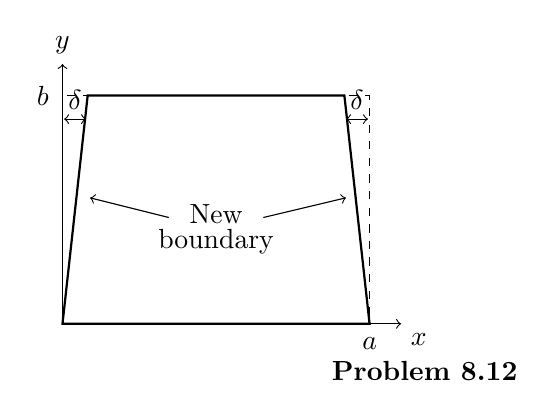
\begin{tikzpicture}[scale=1.0]
  % axes
  \draw[->] (0,0) -- (4.3,0) node[below right] {$x$};
  \draw[->] (0,0) -- (0,3.3) node[above] {$y$};
  \node[below] at (3.9,-0.05) {$a$};
  \node[left] at (-0.05,2.9) {$b$};
  % dashed original rectangle
  \draw[dashed] (0,0) rectangle (3.9,2.9);
  % new boundary: trapezoid wider at bottom, narrower at top
  \draw[thick] (0,0) -- (0.32,2.9) -- (3.58,2.9) -- (3.9,0) -- cycle;
  % delta marks at top corners
  \draw[<->] (0.02,2.6) -- (0.3,2.6);
  \node at (0.16,2.85) {$\delta$};
  \draw[<->] (3.88,2.6) -- (3.6,2.6);
  \node at (3.74,2.85) {$\delta$};
  % new boundary label with arrows to slanted sides
  \node at (1.95,1.4) {New};
  \node at (1.95,1.05) {boundary};
  \draw[->] (1.35,1.35) -- (0.35,1.6);
  \draw[->] (2.55,1.35) -- (3.6,1.6);
  \node at (4.6,-0.6) {\textbf{Problem 8.12}};
\end{tikzpicture}
\end{center}
\solution

Take the normal outward from the guide cross section and let a positive
$\delta(s)$ expand the domain.  Write
$\psi=\psi_0+\delta\psi$ and
$\gamma^2=\gamma_0^2+\delta\gamma^2$.
\textbf{(a)} Subtract the two transverse Helmholtz equations and
use Green's identity on the original domain:
\[
\delta\gamma^2\int_{S_0}|\psi_0|^2dA
=-\oint_{C_0}\left[\psi_0^*\partial_n\delta\psi
-\delta\psi\,\partial_n\psi_0^*\right]dl+O(\delta^2).
\]
For TM, the displaced Dirichlet condition is
$\delta\psi=-\delta\,\partial_n\psi_0$ on $C_0$.
Since $\psi_0=0$ there, substitution gives
\[
\delta\gamma^2=-\frac{\oint\delta|\partial_n\psi_0|^2dl}{N},
\qquad N=\int|\psi_0|^2dA.
\]
For TE, the displaced outward normal is
$\mathbf n-\delta'(s)\mathbf t$ to first order.  Expansion of the
Neumann condition therefore gives
\[
\partial_n\delta\psi=-\delta\partial_n^2\psi_0
+\delta'\partial_s\psi_0.
\]
Under the problem's assumption that $\delta'$ is higher order, omit
the last term.  Then
$\delta\gamma^2=\oint\delta\psi_0^*\partial_n^2\psi_0dl/N$,
which together with the TM result proves the displayed formula.
For a general deformation the slope term must be retained.  An
integration by parts around the contour, using
$\partial_n^2\psi_0=-\gamma_0^2\psi_0-\partial_s^2\psi_0$
on a Neumann boundary, gives the more general form
\[
\boxed{\delta\gamma_{\rm TE}^2=
\frac{\oint\delta[|\partial_s\psi_0|^2-\gamma_0^2|\psi_0|^2]dl}{N}.}
\]
This qualification matters for the ellipse in Problem 8.13.

\textbf{(b)} Let the positive symbol $\delta$ in the sketch denote
the inward displacement at either top corner.  The two side
boundaries move by the outward-normal amount
$\delta_n(y)=-\delta y/b$; the horizontal boundaries do not move.
Assume $a>b$ so that the stated $\mathrm{TE}_{10}$ mode is
nondegenerate.  Its unperturbed field is
$\psi_0=\cos(\pi x/a)$, with $N=ab/2$.
On the sloping sides $\partial_s\psi_0=0$ and
$\psi_0\partial_n^2\psi_0=-\pi^2/a^2$, so the slope correction
vanishes even though $\delta_n'$ is first order.  Thus
\[
\delta\gamma_{\rm TE}^2
=\frac{2\int_0^b(-\delta y/b)(-\pi^2/a^2)dy}{ab/2}
=\frac{2\pi^2\delta}{a^3}.
\]
For $\mathrm{TM}_{11}$,
$\psi_0=\sin(\pi x/a)\sin(\pi y/b)$ and $N=ab/4$.
On either side $(\partial_n\psi_0)^2=(\pi/a)^2\sin^2(\pi y/b)$.
Using $\int_0^by\sin^2(\pi y/b)dy=b^2/4$ gives the same shift.
Therefore
\[
\boxed{\gamma_{\rm TE}^2=\frac{\pi^2}{a^2}
\left(1+\frac{2\delta}{a}\right)+O(\delta^2),\qquad
\gamma_{\rm TM}^2=\frac{\pi^2}{a^2}+\frac{\pi^2}{b^2}
+\frac{2\pi^2\delta}{a^3}+O(\delta^2).}
\]
The positive shifts agree with the reduction in mean width from $a$
to $a-\delta$.  For a square, the degenerate TE pair must instead
be treated together as in Problem 8.13.

\Needspace{5\baselineskip}
\par\bigskip
\noindent\textbf{8.13}\quad To treat perturbations if there is a degeneracy of modes in guides or cavities under ideal conditions, one must use degenerate-state perturbation theory. Consider the two-dimensional (waveguide) situation in which there is an $N$-fold degeneracy in the ideal circumstances (of perfect conductivity or chosen shape of cross section), with no other nearby modes. There are $N$ linearly independent solutions $\psi_{0}^{(i)}$, chosen to be orthogonal, to the transverse wave equation, $(\nabla_{t}^{2}+\gamma_{0}^{2})\psi_{0}^{(i)}=0$, $i=1,2,\ldots,N$. In response to the perturbation, the degeneracy is in general lifted. There is a set of perturbed eigenvalues, $\gamma_{k}^{2}$, with associated eigenmodes, $\psi_{k}$, which can be expanded (in lowest order) in terms of the $N$ unperturbed eigenmodes: $\psi_{k}=\sum_{i}a_{i}\psi_{0}^{(i)}$.
\begin{enumerate}
\item[(a)] Show that the generalization of (8.68) for finite conductivity (and the corresponding expression in Problem 8.12 on distortion of the shape of a waveguide) is the set of algebraic equations,
\[
\sum_{i=1}^{N}\;[(\gamma^{2}-\gamma_{0}^{2})N_{j}\delta_{ji}+\Delta_{ji}]a_{i}=0\qquad(j=1,2,\ldots,N)
\]
where
\[
N_{j}=\int_{A}|\psi_{0}^{(j)}|^{2}\;da\qquad\text{and}\qquad
\Delta_{ji}=f\oint_{C}\frac{\partial\psi_{0}^{(j)*}}{\partial n}\,\frac{\partial\psi_{0}^{(i)}}{\partial n}\;dl
\]
for finite conductivity \erratum{of TM modes (as in Eq.~(8.68))}, and
\[
\Delta_{ji}=\oint_C\delta\left[
\partial_n\psi_0^{(j)*}\partial_n\psi_0^{(i)}
-\psi_0^{(j)*}\partial_n^2\psi_0^{(i)}\right]dl
+\erratum{\oint_C\frac{d\delta}{ds}\,
\psi_0^{(j)*}\partial_s\psi_0^{(i)}\,dl}
\]
for distortion of the boundary shape. \erratum{The extra term accounts
for rotation of the normal. It vanishes for TM modes and may be
neglected for TE modes only under the higher-order slope assumption
of Problem 8.12. That assumption does not apply to the ellipse in (b).}
\item[(b)] The lowest mode in a circular guide of radius $R$ is the twofold degenerate $\mathrm{TE}_{11}$ mode, with fields given by
\[
\psi^{(\pm)}=B_{z}=B_{0}J_{1}(\gamma_{0}\rho)\,\exp(\pm i\phi)\,\exp(ikz-i\omega t)
\]
The eigenvalue parameter is $\gamma_{0}=1.841/R$, corresponding to the first root of $dJ_{1}(x)/dx$. Suppose that the circular waveguide is distorted along its length into an elliptical shape with semimajor and semiminor axes, $a=R+\Delta R$, $b=R-\Delta R$, respectively. To first order in $\Delta R/R$, the area and circumference of the guide remain unchanged. Show that the degeneracy is lifted by the distortion and that to first order in $\Delta R/R$, $\gamma_{1}^{2}=\gamma_{0}^{2}(1+\lambda\Delta R/R)$ and $\gamma_{2}^{2}=\gamma_{0}^{2}(1-\lambda\Delta R/R)$. Determine the numerical value of $\lambda$ and find the eigenmodes as linear combinations of $\psi^{(\pm)}$. Explain physically why the eigenmodes turn out as they do.
\end{enumerate}
\solution

\textbf{(a)} Multiply the perturbed wave equation by
$\psi_0^{(j)*}$, subtract its unperturbed adjoint equation, and
integrate over the cross section.  Orthogonality makes the volume
term $(\gamma^2-\gamma_0^2)N_ja_j$.  Linearizing the boundary
condition supplies a boundary term linear in every $a_i$.
For the TM surface-impedance condition of Eq.~(8.65), with its
normal directed \emph{into} the guide, the boundary value is
$f\partial_n\psi_0$.  Equivalently, with the outward normal used
here it is $-f\partial_n\psi_0$.  Green's identity therefore gives
\[
\sum_i[(\gamma^2-\gamma_0^2)N_j\delta_{ji}+\Delta_{ji}]a_i=0,
\qquad
\Delta_{ji}=f\oint\partial_n\psi_0^{(j)*}\partial_n\psi_0^{(i)}dl.
\]
Normal reversal has no effect on the product of the two derivatives.
This quoted finite-conductivity formula is the TM formula; setting
Neumann derivatives to zero does not describe TE conductor loss.
For TE the surface-impedance perturbation gives instead
\[
\Delta^{\rm TE}_{ji}=(1+i)\frac{R_s\gamma_0^2}{\omega\mu}
\oint\left[\psi_0^{(j)*}\psi_0^{(i)}
+\frac{k^2}{\gamma_0^4}\partial_s\psi_0^{(j)*}\partial_s\psi_0^{(i)}\right]dl.
\]
For a diagonal matrix element this yields
$\delta\gamma^2=-2(1+i)k\beta$, with $\beta$ obtained by the
surface-loss calculation in Problem 8.4.  To see the off-diagonal
terms, take $\psi=B_z$ as in (8.36) and in part (b), and form
an arbitrary superposition $\psi=\sum_i a_i\psi_i$.
Its wall-current norm is the quadratic form
\[
\oint|\mathbf H_\parallel|^2dl=
\frac1{\mu^2}\sum_{j,i}a_j^*a_i\oint\left[\psi_j^*\psi_i+
\frac{k^2}{\gamma_0^4}(\partial_s\psi_j^*)(\partial_s\psi_i)\right]dl.
\]
Here $\parallel$ means tangential to the conducting wall. Its
longitudinal and contour-tangent magnetic-field components are
orthogonal, giving the two terms. The factor $1/\mu^2$ converts
$\mathbf B$ to $\mathbf H$. The modal power is
$(\omega k/2\mu\gamma_0^2)\sum_iN_i|a_i|^2$.
Equating $2\beta P$ to $(R_s/2)\oint|\mathbf H_\parallel|^2dl$
fixes the dissipative quadratic form; the equal reactive and
resistive parts of a good conductor supply its factor $1+i$.
Since this holds for every set of complex $a_i$, polarization of
the quadratic form fixes every matrix element as displayed.
If TE and TM families are mutually degenerate, both sets of fields
and their mutual surface-current overlaps must be included.

For a displaced boundary the Dirichlet calculation gives
$\Delta_{ji}=\oint\delta\partial_n\psi_j^*\partial_n\psi_i dl$.
The general Neumann calculation in Problem 8.12 gives
\begin{align*}
\Delta_{ji}^{\rm TE}
&=-\oint\delta\psi_j^*\partial_n^2\psi_i dl
+\oint\delta'\psi_j^*\partial_s\psi_i dl\\
&=\oint\delta\left[\gamma_0^2\psi_j^*\psi_i
-\partial_s\psi_j^*\partial_s\psi_i\right]dl.
\end{align*}
The second line follows by integrating the tangential second
derivative by parts.  It is Hermitian for a real shape perturbation.
When $\delta'$ is of higher order, the first line reduces to the
shape formula originally quoted.  For finite-conductivity TM modes
and either shape problem, nontrivial coefficients require
\[
\det[(\gamma^2-\gamma_0^2)\mathbf N+\boldsymbol\Delta]=0.
\]
Equivalently, diagonalize
$\mathbf N^{-1/2}\boldsymbol\Delta\mathbf N^{-1/2}$; its negative
eigenvalues are the first-order shifts of $\gamma^2$.

\textbf{(b)} Put $x=x'_{11}=1.841183781$ and suppress the common
$z,t$ factors.  To first order the ellipse is the radial deformation
$\delta(\phi)=\Delta R\cos2\phi$.  Its tangential derivative is
$\delta'=-2(\Delta R/R)\sin2\phi$, of the same perturbative order;
it cannot be discarded.  In the basis
$\psi_\pm=B_0J_1(\gamma_0\rho)e^{\pm i\phi}$, both norms are
\[
N=\pi R^2|B_0J_1(x)|^2(1-x^{-2}).
\]
The diagonal shape matrix elements vanish because the integrals of
$\cos2\phi$ vanish.  For the off-diagonal element,
$\psi_+^*\psi_-=|B_0J_1(x)|^2e^{-2i\phi}$ and
$\partial_s\psi_+^*\partial_s\psi_-=-R^{-2}\psi_+^*\psi_-$.
Since $\int_0^{2\pi}\cos2\phi\,e^{-2i\phi}d\phi=\pi$,
\[
\Delta_{+-}=\Delta_{-+}
=\pi R\Delta R|B_0J_1(x)|^2(\gamma_0^2+R^{-2}).
\]
The combinations $(\psi_++\psi_-)/\sqrt2\propto\cos\phi$
and $(\psi_+-\psi_-)/(i\sqrt2)\propto\sin\phi$ diagonalize this
matrix.  Their shifts are
\[
\boxed{\gamma_{\cos}^2=\gamma_0^2
\left(1-\lambda\frac{\Delta R}{R}\right),\qquad
\gamma_{\sin}^2=\gamma_0^2
\left(1+\lambda\frac{\Delta R}{R}\right),\quad
\lambda=\frac{x^2+1}{x^2-1}=1.836834889.}
\]
The reflection axes of the ellipse select standing angular patterns;
a traveling $e^{\pm i\phi}$ pattern no longer has a single
eigenvalue.  The $\cos\phi$ longitudinal magnetic field varies
mainly across the longer $x$ direction and has the lower transverse
wave number; its electric field is predominantly along $y$.
The other polarization has the opposite ordering.

As an independent check, map the ellipse to the unit disk by
$x=(1+\varepsilon)X$, $y=(1-\varepsilon)Y$.
The Neumann Rayleigh quotient changes by
\[
\delta\gamma^2=\frac{2\varepsilon
\int(|\partial_Y\psi|^2-|\partial_X\psi|^2)dA}{\int|\psi|^2dA}.
\]
For $J_1(x\rho/R)\cos\phi$, direct radial and angular integration
gives $-1.836834889\,\varepsilon\gamma_0^2$, agreeing with the
complete boundary perturbation.  Omitting normal rotation would
instead give $\lambda=1$, which fails this independent check.

\Needspace{5\baselineskip}
\par\bigskip
\noindent\textbf{8.14}\quad Consider an optical fiber with a graded index of refraction for rays confined to the $x$-$z$ plane, $n(x)=n(0)\,\mathrm{sech}(\alpha x)$. The fiber has large enough transverse dimensions ($x$) to contain all rays of interest, which are evidently symmetric about $x=0$. The invariant $\bar{n}=n(x_{\max})=n(0)\cos\theta(0)$.
\begin{enumerate}
\item[(a)] Solve the eikonal equations for the transverse coordinate $x(z)$ of the ray and show that
\[
\alpha x=\sinh^{-1}[\sinh(\alpha x_{\max})\,\sin(\alpha z)]
\]
where the origin in $z$ is chosen when the ray has $x=0$. Sketch rays over one half-period for ``launch angles'' $\theta(0)=\pi/6$, $\pi/4$, and $\pi/3$.
\item[(b)] Find the half-period $Z$ of the ray. Does it depend on $\bar{n}$?
\item[(c)] Show that the optical path length for a half period, $L_{\mathrm{opt}}=\int n(x)\;ds$ is $L_{\mathrm{opt}}=n(0)Z$. Comment on the effectiveness of this particular grading of the index.
\end{enumerate}
\emph{Hint}: In the computation of $L_{\mathrm{opt}}$, a useful change of variables is $\sinh(\alpha x)=\sinh(\alpha x_{\max})\sin t$. The resulting integral can be done by contour integration:
\[
\int_{0}^{\pi/2}\frac{d\theta}{1+a^{2}\sin^{2}\theta}=\frac{\pi}{2\sqrt{1+a^{2}}}
\]
\solution

\medskip\noindent\textbf{(a)} Write $n_0=n(0)$, $\theta_0=\theta(0)$ and take $0\leq\theta_0<\pi/2$.
The eikonal equation $d(n\widehat{\mathbf t})/ds=\nabla n$
has a conserved $z$ component,
\[
n\frac{dz}{ds}=\bar n=n_0\cos\theta_0.
\]
Thus $dx/dz=\pm\sqrt{n^2/\bar n^2-1}$.  With
$A=\tan\theta_0=\sinh(\alpha x_{\max})$ and
$y=\sinh(\alpha x)$ this becomes
\[
\left(\frac{dy}{dz}\right)^2
=\alpha^2\left[A^2-y^2\right].
\]
Starting at $x(0)=0$ with positive slope gives $y=A\sin\alpha z$;
continuing smoothly through the turning point gives
\[
\boxed{x(z)=\alpha^{-1}\operatorname{arsinh}
 [\tan\theta_0\sin(\alpha z)].}
\]
The three requested rays are plotted below.  Their different heights
are $\alpha x_{\max}=\operatorname{arsinh}(\tan\theta_0)$.
\begin{center}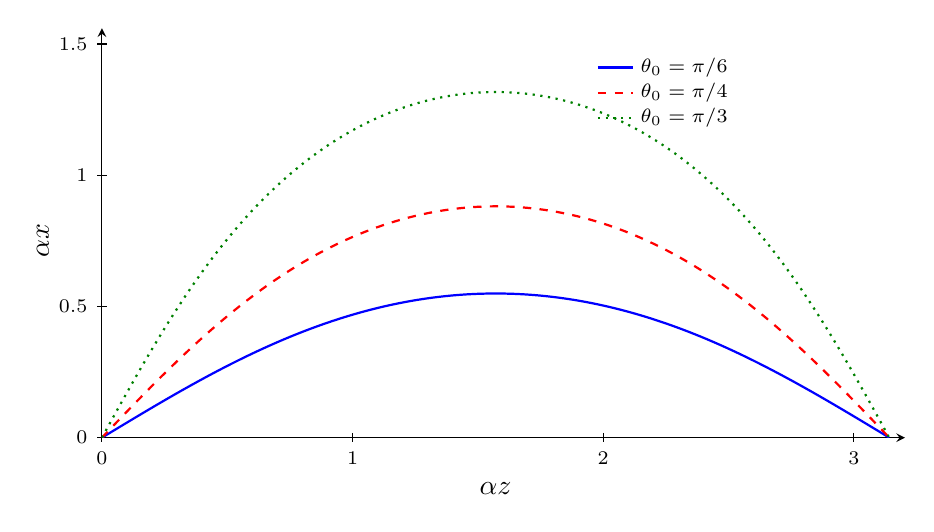
\begin{tikzpicture}[x=1cm,y=1cm,>=stealth]
\draw[->] (0,0)--(10.2,0);
\draw[->] (0,0)--(0,5.2);
\draw (0.00000,.06)--(0.00000,-.06) node[below] {\scriptsize $0$};
\draw (3.18310,.06)--(3.18310,-.06) node[below] {\scriptsize $1$};
\draw (6.36620,.06)--(6.36620,-.06) node[below] {\scriptsize $2$};
\draw (9.54930,.06)--(9.54930,-.06) node[below] {\scriptsize $3$};
\draw (.06,0.00000)--(-.06,0.00000) node[left] {\scriptsize $0$};
\draw (.06,1.66667)--(-.06,1.66667) node[left] {\scriptsize $0.5$};
\draw (.06,3.33333)--(-.06,3.33333) node[left] {\scriptsize $1$};
\draw (.06,5.00000)--(-.06,5.00000) node[left] {\scriptsize $1.5$};
\node[below] at (5.0,-.45) {$\alpha z$};
\node[rotate=90] at (-.75,2.5) {$\alpha x$};
\begin{scope}
\clip (0,0) rectangle (10,5);
\draw[blue,thick] plot coordinates {(0.000000,0.000000) (0.033333,0.020153) (0.066667,0.040303) (0.100000,0.060447) (0.133333,0.080582) (0.166667,0.100705) (0.200000,0.120814) (0.233333,0.140905) (0.266667,0.160976) (0.300000,0.181023) (0.333333,0.201043) (0.366667,0.221035) (0.400000,0.240994) (0.433333,0.260918) (0.466667,0.280805) (0.500000,0.300650) (0.533333,0.320453) (0.566667,0.340209) (0.600000,0.359916) (0.633333,0.379571) (0.666667,0.399172) (0.700000,0.418715) (0.733333,0.438198) (0.766667,0.457619) (0.800000,0.476975) (0.833333,0.496262) (0.866667,0.515479) (0.900000,0.534624) (0.933333,0.553692) (0.966667,0.572683) (1.000000,0.591593) (1.033333,0.610420) (1.066667,0.629162) (1.100000,0.647816) (1.133333,0.666380) (1.166667,0.684851) (1.200000,0.703228) (1.233333,0.721508) (1.266667,0.739688) (1.300000,0.757768) (1.333333,0.775744) (1.366667,0.793614) (1.400000,0.811377) (1.433333,0.829029) (1.466667,0.846571) (1.500000,0.863998) (1.533333,0.881310) (1.566667,0.898504) (1.600000,0.915579) (1.633333,0.932533) (1.666667,0.949364) (1.700000,0.966069) (1.733333,0.982649) (1.766667,0.999100) (1.800000,1.015421) (1.833333,1.031611) (1.866667,1.047668) (1.900000,1.063590) (1.933333,1.079377) (1.966667,1.095025) (2.000000,1.110535) (2.033333,1.125904) (2.066667,1.141131) (2.100000,1.156215) (2.133333,1.171155) (2.166667,1.185949) (2.200000,1.200596) (2.233333,1.215094) (2.266667,1.229443) (2.300000,1.243642) (2.333333,1.257689) (2.366667,1.271582) (2.400000,1.285323) (2.433333,1.298908) (2.466667,1.312337) (2.500000,1.325609) (2.533333,1.338723) (2.566667,1.351679) (2.600000,1.364475) (2.633333,1.377110) (2.666667,1.389584) (2.700000,1.401895) (2.733333,1.414043) (2.766667,1.426028) (2.800000,1.437848) (2.833333,1.449502) (2.866667,1.460990) (2.900000,1.472312) (2.933333,1.483466) (2.966667,1.494452) (3.000000,1.505269) (3.033333,1.515917) (3.066667,1.526395) (3.100000,1.536703) (3.133333,1.546840) (3.166667,1.556805) (3.200000,1.566598) (3.233333,1.576218) (3.266667,1.585666) (3.300000,1.594939) (3.333333,1.604039) (3.366667,1.612965) (3.400000,1.621716) (3.433333,1.630291) (3.466667,1.638691) (3.500000,1.646916) (3.533333,1.654963) (3.566667,1.662835) (3.600000,1.670529) (3.633333,1.678046) (3.666667,1.685385) (3.700000,1.692546) (3.733333,1.699530) (3.766667,1.706334) (3.800000,1.712961) (3.833333,1.719408) (3.866667,1.725676) (3.900000,1.731764) (3.933333,1.737673) (3.966667,1.743402) (4.000000,1.748951) (4.033333,1.754320) (4.066667,1.759508) (4.100000,1.764516) (4.133333,1.769343) (4.166667,1.773989) (4.200000,1.778454) (4.233333,1.782738) (4.266667,1.786840) (4.300000,1.790761) (4.333333,1.794501) (4.366667,1.798058) (4.400000,1.801434) (4.433333,1.804628) (4.466667,1.807640) (4.500000,1.810470) (4.533333,1.813117) (4.566667,1.815582) (4.600000,1.817865) (4.633333,1.819966) (4.666667,1.821884) (4.700000,1.823620) (4.733333,1.825173) (4.766667,1.826543) (4.800000,1.827731) (4.833333,1.828736) (4.866667,1.829558) (4.900000,1.830198) (4.933333,1.830655) (4.966667,1.830929) (5.000000,1.831020) (5.033333,1.830929) (5.066667,1.830655) (5.100000,1.830198) (5.133333,1.829558) (5.166667,1.828736) (5.200000,1.827731) (5.233333,1.826543) (5.266667,1.825173) (5.300000,1.823620) (5.333333,1.821884) (5.366667,1.819966) (5.400000,1.817865) (5.433333,1.815582) (5.466667,1.813117) (5.500000,1.810470) (5.533333,1.807640) (5.566667,1.804628) (5.600000,1.801434) (5.633333,1.798058) (5.666667,1.794501) (5.700000,1.790761) (5.733333,1.786840) (5.766667,1.782738) (5.800000,1.778454) (5.833333,1.773989) (5.866667,1.769343) (5.900000,1.764516) (5.933333,1.759508) (5.966667,1.754320) (6.000000,1.748951) (6.033333,1.743402) (6.066667,1.737673) (6.100000,1.731764) (6.133333,1.725676) (6.166667,1.719408) (6.200000,1.712961) (6.233333,1.706334) (6.266667,1.699530) (6.300000,1.692546) (6.333333,1.685385) (6.366667,1.678046) (6.400000,1.670529) (6.433333,1.662835) (6.466667,1.654963) (6.500000,1.646916) (6.533333,1.638691) (6.566667,1.630291) (6.600000,1.621716) (6.633333,1.612965) (6.666667,1.604039) (6.700000,1.594939) (6.733333,1.585666) (6.766667,1.576218) (6.800000,1.566598) (6.833333,1.556805) (6.866667,1.546840) (6.900000,1.536703) (6.933333,1.526395) (6.966667,1.515917) (7.000000,1.505269) (7.033333,1.494452) (7.066667,1.483466) (7.100000,1.472312) (7.133333,1.460990) (7.166667,1.449502) (7.200000,1.437848) (7.233333,1.426028) (7.266667,1.414043) (7.300000,1.401895) (7.333333,1.389584) (7.366667,1.377110) (7.400000,1.364475) (7.433333,1.351679) (7.466667,1.338723) (7.500000,1.325609) (7.533333,1.312337) (7.566667,1.298908) (7.600000,1.285323) (7.633333,1.271582) (7.666667,1.257689) (7.700000,1.243642) (7.733333,1.229443) (7.766667,1.215094) (7.800000,1.200596) (7.833333,1.185949) (7.866667,1.171155) (7.900000,1.156215) (7.933333,1.141131) (7.966667,1.125904) (8.000000,1.110535) (8.033333,1.095025) (8.066667,1.079377) (8.100000,1.063590) (8.133333,1.047668) (8.166667,1.031611) (8.200000,1.015421) (8.233333,0.999100) (8.266667,0.982649) (8.300000,0.966069) (8.333333,0.949364) (8.366667,0.932533) (8.400000,0.915579) (8.433333,0.898504) (8.466667,0.881310) (8.500000,0.863998) (8.533333,0.846571) (8.566667,0.829029) (8.600000,0.811377) (8.633333,0.793614) (8.666667,0.775744) (8.700000,0.757768) (8.733333,0.739688) (8.766667,0.721508) (8.800000,0.703228) (8.833333,0.684851) (8.866667,0.666380) (8.900000,0.647816) (8.933333,0.629162) (8.966667,0.610420) (9.000000,0.591593) (9.033333,0.572683) (9.066667,0.553692) (9.100000,0.534624) (9.133333,0.515479) (9.166667,0.496262) (9.200000,0.476975) (9.233333,0.457619) (9.266667,0.438198) (9.300000,0.418715) (9.333333,0.399172) (9.366667,0.379571) (9.400000,0.359916) (9.433333,0.340209) (9.466667,0.320453) (9.500000,0.300650) (9.533333,0.280805) (9.566667,0.260918) (9.600000,0.240994) (9.633333,0.221035) (9.666667,0.201043) (9.700000,0.181023) (9.733333,0.160976) (9.766667,0.140905) (9.800000,0.120814) (9.833333,0.100705) (9.866667,0.080582) (9.900000,0.060447) (9.933333,0.040303) (9.966667,0.020153) (10.000000,0.000000)};
\draw[red,dashed,thick] plot coordinates {(0.000000,0.000000) (0.033333,0.034905) (0.066667,0.069803) (0.100000,0.104685) (0.133333,0.139545) (0.166667,0.174374) (0.200000,0.209164) (0.233333,0.243910) (0.266667,0.278602) (0.300000,0.313233) (0.333333,0.347797) (0.366667,0.382285) (0.400000,0.416691) (0.433333,0.451008) (0.466667,0.485228) (0.500000,0.519345) (0.533333,0.553351) (0.566667,0.587240) (0.600000,0.621006) (0.633333,0.654641) (0.666667,0.688141) (0.700000,0.721497) (0.733333,0.754705) (0.766667,0.787758) (0.800000,0.820651) (0.833333,0.853377) (0.866667,0.885932) (0.900000,0.918310) (0.933333,0.950506) (0.966667,0.982514) (1.000000,1.014330) (1.033333,1.045949) (1.066667,1.077366) (1.100000,1.108577) (1.133333,1.139578) (1.166667,1.170365) (1.200000,1.200932) (1.233333,1.231278) (1.266667,1.261397) (1.300000,1.291286) (1.333333,1.320943) (1.366667,1.350363) (1.400000,1.379544) (1.433333,1.408482) (1.466667,1.437175) (1.500000,1.465620) (1.533333,1.493814) (1.566667,1.521756) (1.600000,1.549442) (1.633333,1.576870) (1.666667,1.604039) (1.700000,1.630947) (1.733333,1.657591) (1.766667,1.683970) (1.800000,1.710082) (1.833333,1.735926) (1.866667,1.761500) (1.900000,1.786803) (1.933333,1.811834) (1.966667,1.836592) (2.000000,1.861076) (2.033333,1.885284) (2.066667,1.909215) (2.100000,1.932870) (2.133333,1.956247) (2.166667,1.979346) (2.200000,2.002166) (2.233333,2.024706) (2.266667,2.046967) (2.300000,2.068947) (2.333333,2.090647) (2.366667,2.112066) (2.400000,2.133204) (2.433333,2.154060) (2.466667,2.174636) (2.500000,2.194930) (2.533333,2.214942) (2.566667,2.234674) (2.600000,2.254124) (2.633333,2.273292) (2.666667,2.292180) (2.700000,2.310787) (2.733333,2.329113) (2.766667,2.347158) (2.800000,2.364923) (2.833333,2.382409) (2.866667,2.399614) (2.900000,2.416540) (2.933333,2.433188) (2.966667,2.449556) (3.000000,2.465646) (3.033333,2.481458) (3.066667,2.496993) (3.100000,2.512251) (3.133333,2.527232) (3.166667,2.541936) (3.200000,2.556365) (3.233333,2.570519) (3.266667,2.584398) (3.300000,2.598002) (3.333333,2.611332) (3.366667,2.624389) (3.400000,2.637173) (3.433333,2.649684) (3.466667,2.661923) (3.500000,2.673891) (3.533333,2.685587) (3.566667,2.697013) (3.600000,2.708169) (3.633333,2.719054) (3.666667,2.729671) (3.700000,2.740019) (3.733333,2.750099) (3.766667,2.759910) (3.800000,2.769455) (3.833333,2.778732) (3.866667,2.787743) (3.900000,2.796487) (3.933333,2.804966) (3.966667,2.813180) (4.000000,2.821128) (4.033333,2.828812) (4.066667,2.836232) (4.100000,2.843388) (4.133333,2.850281) (4.166667,2.856910) (4.200000,2.863277) (4.233333,2.869381) (4.266667,2.875224) (4.300000,2.880804) (4.333333,2.886123) (4.366667,2.891181) (4.400000,2.895977) (4.433333,2.900513) (4.466667,2.904788) (4.500000,2.908804) (4.533333,2.912559) (4.566667,2.916054) (4.600000,2.919289) (4.633333,2.922266) (4.666667,2.924982) (4.700000,2.927440) (4.733333,2.929638) (4.766667,2.931578) (4.800000,2.933259) (4.833333,2.934681) (4.866667,2.935844) (4.900000,2.936749) (4.933333,2.937395) (4.966667,2.937783) (5.000000,2.937912) (5.033333,2.937783) (5.066667,2.937395) (5.100000,2.936749) (5.133333,2.935844) (5.166667,2.934681) (5.200000,2.933259) (5.233333,2.931578) (5.266667,2.929638) (5.300000,2.927440) (5.333333,2.924982) (5.366667,2.922266) (5.400000,2.919289) (5.433333,2.916054) (5.466667,2.912559) (5.500000,2.908804) (5.533333,2.904788) (5.566667,2.900513) (5.600000,2.895977) (5.633333,2.891181) (5.666667,2.886123) (5.700000,2.880804) (5.733333,2.875224) (5.766667,2.869381) (5.800000,2.863277) (5.833333,2.856910) (5.866667,2.850281) (5.900000,2.843388) (5.933333,2.836232) (5.966667,2.828812) (6.000000,2.821128) (6.033333,2.813180) (6.066667,2.804966) (6.100000,2.796487) (6.133333,2.787743) (6.166667,2.778732) (6.200000,2.769455) (6.233333,2.759910) (6.266667,2.750099) (6.300000,2.740019) (6.333333,2.729671) (6.366667,2.719054) (6.400000,2.708169) (6.433333,2.697013) (6.466667,2.685587) (6.500000,2.673891) (6.533333,2.661923) (6.566667,2.649684) (6.600000,2.637173) (6.633333,2.624389) (6.666667,2.611332) (6.700000,2.598002) (6.733333,2.584398) (6.766667,2.570519) (6.800000,2.556365) (6.833333,2.541936) (6.866667,2.527232) (6.900000,2.512251) (6.933333,2.496993) (6.966667,2.481458) (7.000000,2.465646) (7.033333,2.449556) (7.066667,2.433188) (7.100000,2.416540) (7.133333,2.399614) (7.166667,2.382409) (7.200000,2.364923) (7.233333,2.347158) (7.266667,2.329113) (7.300000,2.310787) (7.333333,2.292180) (7.366667,2.273292) (7.400000,2.254124) (7.433333,2.234674) (7.466667,2.214942) (7.500000,2.194930) (7.533333,2.174636) (7.566667,2.154060) (7.600000,2.133204) (7.633333,2.112066) (7.666667,2.090647) (7.700000,2.068947) (7.733333,2.046967) (7.766667,2.024706) (7.800000,2.002166) (7.833333,1.979346) (7.866667,1.956247) (7.900000,1.932870) (7.933333,1.909215) (7.966667,1.885284) (8.000000,1.861076) (8.033333,1.836592) (8.066667,1.811834) (8.100000,1.786803) (8.133333,1.761500) (8.166667,1.735926) (8.200000,1.710082) (8.233333,1.683970) (8.266667,1.657591) (8.300000,1.630947) (8.333333,1.604039) (8.366667,1.576870) (8.400000,1.549442) (8.433333,1.521756) (8.466667,1.493814) (8.500000,1.465620) (8.533333,1.437175) (8.566667,1.408482) (8.600000,1.379544) (8.633333,1.350363) (8.666667,1.320943) (8.700000,1.291286) (8.733333,1.261397) (8.766667,1.231278) (8.800000,1.200932) (8.833333,1.170365) (8.866667,1.139578) (8.900000,1.108577) (8.933333,1.077366) (8.966667,1.045949) (9.000000,1.014330) (9.033333,0.982514) (9.066667,0.950506) (9.100000,0.918310) (9.133333,0.885932) (9.166667,0.853377) (9.200000,0.820651) (9.233333,0.787758) (9.266667,0.754705) (9.300000,0.721497) (9.333333,0.688141) (9.366667,0.654641) (9.400000,0.621006) (9.433333,0.587240) (9.466667,0.553351) (9.500000,0.519345) (9.533333,0.485228) (9.566667,0.451008) (9.600000,0.416691) (9.633333,0.382285) (9.666667,0.347797) (9.700000,0.313233) (9.733333,0.278602) (9.766667,0.243910) (9.800000,0.209164) (9.833333,0.174374) (9.866667,0.139545) (9.900000,0.104685) (9.933333,0.069803) (9.966667,0.034905) (10.000000,0.000000)};
\draw[green!50!black,dotted,thick] plot coordinates {(0.000000,0.000000) (0.033333,0.060456) (0.066667,0.120885) (0.100000,0.181261) (0.133333,0.241558) (0.166667,0.301749) (0.200000,0.361810) (0.233333,0.421715) (0.266667,0.481439) (0.300000,0.540957) (0.333333,0.600246) (0.366667,0.659283) (0.400000,0.718046) (0.433333,0.776512) (0.466667,0.834661) (0.500000,0.892474) (0.533333,0.949930) (0.566667,1.007011) (0.600000,1.063701) (0.633333,1.119983) (0.666667,1.175841) (0.700000,1.231260) (0.733333,1.286227) (0.766667,1.340729) (0.800000,1.394755) (0.833333,1.448292) (0.866667,1.501332) (0.900000,1.553864) (0.933333,1.605881) (0.966667,1.657374) (1.000000,1.708338) (1.033333,1.758764) (1.066667,1.808650) (1.100000,1.857989) (1.133333,1.906777) (1.166667,1.955012) (1.200000,2.002690) (1.233333,2.049809) (1.266667,2.096368) (1.300000,2.142365) (1.333333,2.187799) (1.366667,2.232671) (1.400000,2.276980) (1.433333,2.320727) (1.466667,2.363913) (1.500000,2.406539) (1.533333,2.448607) (1.566667,2.490118) (1.600000,2.531074) (1.633333,2.571478) (1.666667,2.611332) (1.700000,2.650639) (1.733333,2.689403) (1.766667,2.727625) (1.800000,2.765310) (1.833333,2.802460) (1.866667,2.839079) (1.900000,2.875171) (1.933333,2.910740) (1.966667,2.945788) (2.000000,2.980321) (2.033333,3.014341) (2.066667,3.047853) (2.100000,3.080860) (2.133333,3.113368) (2.166667,3.145378) (2.200000,3.176897) (2.233333,3.207927) (2.266667,3.238472) (2.300000,3.268537) (2.333333,3.298126) (2.366667,3.327243) (2.400000,3.355890) (2.433333,3.384074) (2.466667,3.411796) (2.500000,3.439062) (2.533333,3.465874) (2.566667,3.492238) (2.600000,3.518156) (2.633333,3.543632) (2.666667,3.568669) (2.700000,3.593273) (2.733333,3.617445) (2.766667,3.641189) (2.800000,3.664510) (2.833333,3.687409) (2.866667,3.709892) (2.900000,3.731960) (2.933333,3.753617) (2.966667,3.774866) (3.000000,3.795711) (3.033333,3.816154) (3.066667,3.836199) (3.100000,3.855848) (3.133333,3.875104) (3.166667,3.893970) (3.200000,3.912448) (3.233333,3.930543) (3.266667,3.948255) (3.300000,3.965588) (3.333333,3.982544) (3.366667,3.999126) (3.400000,4.015336) (3.433333,4.031176) (3.466667,4.046649) (3.500000,4.061757) (3.533333,4.076502) (3.566667,4.090887) (3.600000,4.104912) (3.633333,4.118581) (3.666667,4.131896) (3.700000,4.144857) (3.733333,4.157468) (3.766667,4.169729) (3.800000,4.181644) (3.833333,4.193212) (3.866667,4.204437) (3.900000,4.215319) (3.933333,4.225860) (3.966667,4.236061) (4.000000,4.245925) (4.033333,4.255452) (4.066667,4.264644) (4.100000,4.273502) (4.133333,4.282027) (4.166667,4.290221) (4.200000,4.298084) (4.233333,4.305619) (4.266667,4.312824) (4.300000,4.319703) (4.333333,4.326256) (4.366667,4.332483) (4.400000,4.338385) (4.433333,4.343964) (4.466667,4.349220) (4.500000,4.354154) (4.533333,4.358766) (4.566667,4.363058) (4.600000,4.367029) (4.633333,4.370681) (4.666667,4.374013) (4.700000,4.377027) (4.733333,4.379722) (4.766667,4.382099) (4.800000,4.384159) (4.833333,4.385901) (4.866667,4.387327) (4.900000,4.388435) (4.933333,4.389226) (4.966667,4.389701) (5.000000,4.389860) (5.033333,4.389701) (5.066667,4.389226) (5.100000,4.388435) (5.133333,4.387327) (5.166667,4.385901) (5.200000,4.384159) (5.233333,4.382099) (5.266667,4.379722) (5.300000,4.377027) (5.333333,4.374013) (5.366667,4.370681) (5.400000,4.367029) (5.433333,4.363058) (5.466667,4.358766) (5.500000,4.354154) (5.533333,4.349220) (5.566667,4.343964) (5.600000,4.338385) (5.633333,4.332483) (5.666667,4.326256) (5.700000,4.319703) (5.733333,4.312824) (5.766667,4.305619) (5.800000,4.298084) (5.833333,4.290221) (5.866667,4.282027) (5.900000,4.273502) (5.933333,4.264644) (5.966667,4.255452) (6.000000,4.245925) (6.033333,4.236061) (6.066667,4.225860) (6.100000,4.215319) (6.133333,4.204437) (6.166667,4.193212) (6.200000,4.181644) (6.233333,4.169729) (6.266667,4.157468) (6.300000,4.144857) (6.333333,4.131896) (6.366667,4.118581) (6.400000,4.104912) (6.433333,4.090887) (6.466667,4.076502) (6.500000,4.061757) (6.533333,4.046649) (6.566667,4.031176) (6.600000,4.015336) (6.633333,3.999126) (6.666667,3.982544) (6.700000,3.965588) (6.733333,3.948255) (6.766667,3.930543) (6.800000,3.912448) (6.833333,3.893970) (6.866667,3.875104) (6.900000,3.855848) (6.933333,3.836199) (6.966667,3.816154) (7.000000,3.795711) (7.033333,3.774866) (7.066667,3.753617) (7.100000,3.731960) (7.133333,3.709892) (7.166667,3.687409) (7.200000,3.664510) (7.233333,3.641189) (7.266667,3.617445) (7.300000,3.593273) (7.333333,3.568669) (7.366667,3.543632) (7.400000,3.518156) (7.433333,3.492238) (7.466667,3.465874) (7.500000,3.439062) (7.533333,3.411796) (7.566667,3.384074) (7.600000,3.355890) (7.633333,3.327243) (7.666667,3.298126) (7.700000,3.268537) (7.733333,3.238472) (7.766667,3.207927) (7.800000,3.176897) (7.833333,3.145378) (7.866667,3.113368) (7.900000,3.080860) (7.933333,3.047853) (7.966667,3.014341) (8.000000,2.980321) (8.033333,2.945788) (8.066667,2.910740) (8.100000,2.875171) (8.133333,2.839079) (8.166667,2.802460) (8.200000,2.765310) (8.233333,2.727625) (8.266667,2.689403) (8.300000,2.650639) (8.333333,2.611332) (8.366667,2.571478) (8.400000,2.531074) (8.433333,2.490118) (8.466667,2.448607) (8.500000,2.406539) (8.533333,2.363913) (8.566667,2.320727) (8.600000,2.276980) (8.633333,2.232671) (8.666667,2.187799) (8.700000,2.142365) (8.733333,2.096368) (8.766667,2.049809) (8.800000,2.002690) (8.833333,1.955012) (8.866667,1.906777) (8.900000,1.857989) (8.933333,1.808650) (8.966667,1.758764) (9.000000,1.708338) (9.033333,1.657374) (9.066667,1.605881) (9.100000,1.553864) (9.133333,1.501332) (9.166667,1.448292) (9.200000,1.394755) (9.233333,1.340729) (9.266667,1.286227) (9.300000,1.231260) (9.333333,1.175841) (9.366667,1.119983) (9.400000,1.063701) (9.433333,1.007011) (9.466667,0.949930) (9.500000,0.892474) (9.533333,0.834661) (9.566667,0.776512) (9.600000,0.718046) (9.633333,0.659283) (9.666667,0.600246) (9.700000,0.540957) (9.733333,0.481439) (9.766667,0.421715) (9.800000,0.361810) (9.833333,0.301749) (9.866667,0.241558) (9.900000,0.181261) (9.933333,0.120885) (9.966667,0.060456) (10.000000,0.000000)};
\end{scope}
\draw[blue,thick] (6.3,4.7)--(6.75,4.7);
\node[right,fill=white,inner sep=1pt] at (6.8,4.7) {\scriptsize $\theta_0=\pi/6$};
\draw[red,dashed,thick] (6.3,4.38)--(6.75,4.38);
\node[right,fill=white,inner sep=1pt] at (6.8,4.38) {\scriptsize $\theta_0=\pi/4$};
\draw[green!50!black,dotted,thick] (6.3,4.0600000000000005)--(6.75,4.0600000000000005);
\node[right,fill=white,inner sep=1pt] at (6.8,4.0600000000000005) {\scriptsize $\theta_0=\pi/3$};
\end{tikzpicture}
\end{center}
\medskip\noindent\textbf{(b)} The next crossing of the axis is at
\[
\boxed{Z=\pi/\alpha,}
\]
independent of $\bar n$.  The axial ray is the limiting case of this
family; its transverse oscillation amplitude is zero.

\medskip\noindent\textbf{(c)} For the optical length use $ds/dz=n/\bar n$:
\begin{align*}
L_{\rm opt}
 &=\frac{n_0^2}{\alpha\bar n}
 \int_0^\pi\frac{dt}{1+A^2\sin^2t}\\
 &=\frac{n_0^2}{\alpha\bar n}
 \frac{\pi}{\sqrt{1+A^2}}
 =\boxed{\frac{\pi n_0}{\alpha}=n_0Z}.
\end{align*}
For example the half-range integral follows immediately by
$u=\tan t$:
$\int_0^\infty du/[1+(1+A^2)u^2]=\pi/(2\sqrt{1+A^2})$.
The longer geometrical paths at larger launch angles are exactly
compensated by their lower refractive indices.  In geometrical optics,
with nondispersive $n(x)$, all these rays have the same transit time
$n_0Z/c$ and no differential delay over a half-period.  Material
dispersion and corrections outside the ray approximation are not
included in this conclusion.

\Needspace{5\baselineskip}
\par\bigskip
\noindent\textbf{8.15}\quad Discuss the TE and TM modes in the dielectric slab waveguide of Section 8.11.A as a boundary-value problem.
\begin{enumerate}
\item[(a)] Show that (8.123) emerges as the determining relation for both even and odd modes (in $x$) and that even or odd $p$ goes with the evenness or oddness of the mode, defined by the symmetry in $x$ of the transverse fields.
\item[(b)] Show that the eigenvalues of $\xi$ for the TE modes are given approximately by
\[
\xi\approx\frac{(p+1)\pi}{2(V+1)}\left[1-\frac{(p+1)^{2}\pi^{2}}{24(V+1)^{3}}\right]
\]
The lowest order result is accurate for $V\gg1$ and small $p$. Check the accuracy of the full expression against solution of (8.123) by Newton's method for $V=1,2,3$.
\item[(c)] Calculate the power flow in the $z$ direction (per unit length in the $y$ direction) within the core ($|x|<a$) and in the cladding ($|x|>a$) for the even TE modes and show that the fractions are
\[
F_{\mathrm{core}}=\frac{1}{S}\left[1+\frac{\sin(2V\xi)}{2V\xi}\right]\qquad\text{and}\qquad
F_{\mathrm{clad}}=\frac{1}{S}\left[\frac{\cos^{2}(V\xi)}{V\sqrt{1-\xi^{2}}}\right]
\]
where
\[
S=\left[1+\frac{\sin(2V\xi)}{2V\xi}\right]+\left[\frac{\cos^{2}(V\xi)}{V\sqrt{1-\xi^{2}}}\right]
\]
where $\xi$ is the root of (8.123) for the $p$th mode. Find corresponding expressions for the odd TE modes.
\end{enumerate}
\solution

\medskip\noindent\textbf{(a)} Assume isotropic, lossless, nonmagnetic media, with no variation in $y$.
Set $k_0=\omega/c$ and define
\[
q^2=n_1^2k_0^2-k_z^2,\quad
\beta^2=k_z^2-n_2^2k_0^2,\quad
u=qa=V\xi,\quad w=\beta a=V\sqrt{1-\xi^2}.
\]
Here $u,w>0$ for a bound mode and $u^2+w^2=V^2$.
For TE polarization take $E_y=E_0f(x)e^{ik_zz-i\omega t}$.
In the core, $f=\cos qx$ for even modes or $f=\sin qx$ for odd
modes.  Outside, match to $f(a)e^{-\beta(x-a)}$ at the right
surface and to its parity reflection at the left surface.
Continuity of $E_y$ and $H_z=\partial_xE_y/(i\omega\mu_0)$
requires continuity of $f,f'$.  Therefore
\[
u\tan u=w\quad(\hbox{even TE}),\qquad
-u\cot u=w\quad(\hbox{odd TE}).
\]
For TM polarization replace $E_y$ by $H_y$.  Continuity of $H_y$
and $E_z=-\partial_xH_y/(i\omega\epsilon)$ requires continuity
of $f$ and $f'/\epsilon$, giving the same equations with
$w\mapsto(n_1^2/n_2^2)w$.  The combined result is
\[
\boxed{\tan(V\xi-p\pi/2)=f\,\frac{\sqrt{1-\xi^2}}{\xi},
\quad f=1\ (\mathrm{TE}),\quad f=\frac{n_1^2}{n_2^2}\ (\mathrm{TM}).}
\]
The root belonging to $p$ lies in
$p\pi/2<u<(p+1)\pi/2$; even $p$ is an even transverse field,
and odd $p$ is odd.  The longitudinal component has the opposite
parity, which explains why specifying transverse parity matters.
A bound mode exists when $V>p\pi/2$, with no positive threshold
for $p=0$.

\medskip\noindent\textbf{(b)} For TE modes the phase equation can be written without tangent poles:
since $w/u=\sqrt{1-\xi^2}/\xi$ and $0<\xi<1$,
$\arctan(w/u)=\arccos\xi=\pi/2-\arcsin\xi$. Thus
\[
V\xi+\arcsin\xi=(p+1)\pi/2.
\]
Expanding $\arcsin\xi=\xi+\xi^3/6+O(\xi^5)$ and putting
$A_p=(p+1)\pi/[2(V+1)]$ first on the cubic term gives
\[
\xi=A_p-\frac{A_p^3}{6(V+1)}+\cdots
=\boxed{\frac{(p+1)\pi}{2(V+1)}
 \left[1-\frac{(p+1)^2\pi^2}{24(V+1)^3}\right].}
\]
A stable Newton implementation uses $t=\arccos\xi$ and
$F(t)=V\cos t-t-p\pi/2$, with
\[
t_{j+1}=t_j+\frac{V\cos t_j-t_j-p\pi/2}{V\sin t_j+1}.
\]
The supplementary program retains a bracket $0<t<\pi/2$ and
bisects if a Newton step leaves it.  It gives all bound TE modes
at the requested values:
\begin{center}
\begin{tabular}{rrrrr}
\toprule
$V$&$p$&Newton $\xi$&Approximate $\xi$&Relative error (\%)\\
\midrule
1&0&0.7390851332&0.7450254073&0.8037\\
2&0&0.5149332647&0.5156239102&0.1341\\
2&1&0.9477471335&0.9833986280&3.7617\\
3&0&0.3900403167&0.3901757844&0.0347\\
3&1&0.7596208867&0.7652117854&0.7360\\
\bottomrule
\end{tabular}
\end{center}
The larger error near threshold is expected because $\xi$ is then
near one, outside the small-$\xi$ expansion.

\medskip\noindent\textbf{(c)} The local longitudinal power density is
$S_z=k_z|E_y|^2/(2\omega\mu_0)$.  Let
$P_*=k_z|E_0|^2a/(2\omega\mu_0)$.
For even modes direct integration gives
\begin{align*}
P_{\rm core}&=P_*\int_{-1}^1\cos^2(ut)\,dt
 =P_*\left[1+\frac{\sin2u}{2u}\right],\\
P_{\rm clad}&=\frac{k_z|E_0|^2}{2\omega\mu_0}
 2\cos^2u\int_0^\infty e^{-2\beta x}\,dx
 =P_*\frac{\cos^2u}{w}.
\end{align*}
Dividing by their sum gives precisely the stated fractions.  For
odd modes define
\[
S_o=1-\frac{\sin2u}{2u}+\frac{\sin^2u}{w}.
\]
Then
\[
\boxed{F_{\rm core}^{(o)}=\frac{1-\sin(2u)/(2u)}{S_o},\qquad
F_{\rm clad}^{(o)}=\frac{\sin^2u/w}{S_o}.}
\]
The two claddings are both included.  Their fraction tends to one
at a mode's threshold ($w\downarrow0$), and to zero for a fixed
mode as $V\to\infty$.

\Needspace{5\baselineskip}
\par\bigskip
\noindent\textbf{8.16}\quad The longitudinal phase velocity in the dielectric slab waveguide of the preceding problem is $v_{p}=\omega/k_{z}=c/(n_{1}\cos\theta_{p})$. Intermodal dispersion occurs because the dielectric media have dispersion and also because the group velocity differs intrinsically for different modes.
\begin{enumerate}
\item[(a)] Making the approximation that the dielectrics' dispersion can be neglected, show that the group velocity $v_{g}=d\omega/dk_{z}$ for the $\mathrm{TE}_{p}$ mode is
\[
v_{g}=\frac{c\,\cos\theta_{p}}{n_{1}}\left[\frac{1+\beta_{p}a}{\cos^{2}\theta_{p}+\beta_{p}a}\right]
\]
where $\theta_{p}$ is the eigenangle of the $p$th mode ($\cos\theta_{p}=\sqrt{1-2\Delta\xi_{p}^{2}}$) and $\beta_{p}$ is given by (8.124). Interpret the departure from $v_{p}v_{g}=c^{2}/n_{1}^{2}$ (as in metallic waveguides; $\beta_{p}\to\infty$) in terms of the Goos--H\"anchen effect and ray-like propagation at the simple phase speed $c/n_{1}$. [\emph{Hint}: Write the eigenvalue relation (8.121) in terms of the independent variable $\omega$ and the dependent variable $k_{z}$ and differentiate with respect to $\omega$.]
\item[(b)] Write a program to evaluate $v_{g}$ versus $V/V_{t}$, where $V_{t}=p\pi/2$ is the threshold frequency variable for the $p^{\mathrm{th}}$ mode. Make a plot of $v_{g}/c$ for $n_{1}=1.5$, $n_{2}=1.0$ for $p=0,1,2,\ldots,6$ as a function of $V/V_{t}(p=1)$ on the range $(0,10)$.
\item[(c)] Relate the results of part b to the optical path length difference for the step-index fiber shown in Fig.~8.12b. Can you generate a plot from the results for $v_{g}(p)$ at fixed $V$ for $n_{1}=1.01$, $n_{2}=1.0$ to compare with the ``classical'' ray result?
\end{enumerate}
\solution

\medskip\noindent\textbf{(a)} Keep $n_1,n_2$ independent of frequency, as stipulated.  Put
$W=\omega a/c$, $K=k_za$, $u=qa$, $w=\beta a$ and
$C=\cos\theta_p=K/(n_1W)$.  The TE phase relation is
\[
u=\arctan(w/u)+p\pi/2.
\]
Its differential is
\[
(V^2+w)\,du=u\,dw,
\]
whereas differentiation of
$u^2=n_1^2W^2-K^2$, $w^2=K^2-n_2^2W^2$ gives
\[
u\,du=n_1^2W\,dW-K\,dK,\qquad
w\,dw=K\,dK-n_2^2W\,dW.
\]
Multiplying the differential phase equation by $uw$ and inserting
these two differentials gives
\[
w(V^2+w)(n_1^2W\,dW-K\,dK)
=u^2(K\,dK-n_2^2W\,dW).
\]
The coefficient of $K\,dK$ is $V^2(1+w)$.
Also $n_1^2w^2+n_2^2u^2=(n_1^2-n_2^2)K^2=V^2K^2/W^2$.
Collecting the $dW$ terms and cancelling $V^2$ therefore yields
\[
K\frac{dK}{dW}=\frac{n_1^2Ww+K^2/W}{1+w},\qquad
\frac{dK}{dW}=n_1\frac{C^2+w}{C(1+w)}.
\]
Since $v_g/c=dW/dK$, the result is
\[
\boxed{v_g=\frac{cC}{n_1}\frac{1+w}{C^2+w}.}
\]
In particular
\[
v_pv_g=\frac{c^2}{n_1^2}\frac{1+w}{C^2+w}
>\frac{c^2}{n_1^2}
\]
for a nonaxial, finitely confined mode.  A simple zigzag ray with
speed $c/n_1$ would have $v_{g,z}=cC/n_1$.
The reflection phase varies with $\omega$ and $k_z$, producing a
Goos--H\"anchen displacement.  For TE reflection
$\phi=-2\arctan(\beta/q)$, its displacement along the interface is
\[
-\left.\frac{\partial\phi}{\partial k_z}\right|_\omega
=\frac{2k_z}{q\beta}.
\]
The wave packet thus advances along the interface as well as along
the core ray segments.  The associated cladding field carries part
of the energy in the lower-index medium.  These effects account
for the factor $(1+w)/(C^2+w)>1$; neglecting the reflection-phase
derivative would miss it.  As $w\to\infty$ the core ray expression
is recovered.  At a threshold $w\to0$, $C\to n_2/n_1$ and
$v_g\to c/n_2$, consistently with the energy being mostly outside.

\medskip\noindent\textbf{(b)} The program solves the phase relation independently for each $p$,
then evaluates the boxed expression.  Since $V_t(0)=0$, the common
horizontal scale is $V_t(1)=\pi/2$, as specified in the plot request.
Each higher branch starts at $V/(\pi/2)=p$.
\begin{center}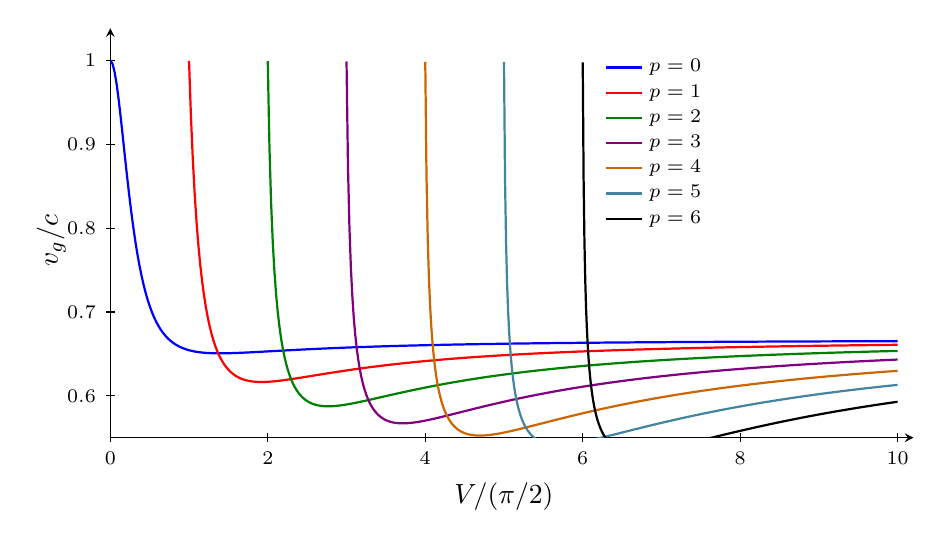
\begin{tikzpicture}[x=1cm,y=1cm,>=stealth]
\draw[->] (0,0)--(10.2,0);
\draw[->] (0,0)--(0,5.2);
\draw (0.00000,.06)--(0.00000,-.06) node[below] {\scriptsize $0$};
\draw (2.00000,.06)--(2.00000,-.06) node[below] {\scriptsize $2$};
\draw (4.00000,.06)--(4.00000,-.06) node[below] {\scriptsize $4$};
\draw (6.00000,.06)--(6.00000,-.06) node[below] {\scriptsize $6$};
\draw (8.00000,.06)--(8.00000,-.06) node[below] {\scriptsize $8$};
\draw (10.00000,.06)--(10.00000,-.06) node[below] {\scriptsize $10$};
\draw (.06,0.53191)--(-.06,0.53191) node[left] {\scriptsize $0.6$};
\draw (.06,1.59574)--(-.06,1.59574) node[left] {\scriptsize $0.7$};
\draw (.06,2.65957)--(-.06,2.65957) node[left] {\scriptsize $0.8$};
\draw (.06,3.72340)--(-.06,3.72340) node[left] {\scriptsize $0.9$};
\draw (.06,4.78723)--(-.06,4.78723) node[left] {\scriptsize $1$};
\node[below] at (5.0,-.45) {$V/(\pi/2)$};
\node[rotate=90] at (-.75,2.5) {$v_g/c$};
\begin{scope}
\clip (0,0) rectangle (10,5);
\draw[blue,thick] plot coordinates {(0.003000,4.786791) (0.029377,4.745172) (0.055755,4.639477) (0.082132,4.478960) (0.108509,4.276425) (0.134887,4.045961) (0.161264,3.800953) (0.187641,3.552764) (0.214018,3.310132) (0.240396,3.079163) (0.266773,2.863653) (0.293150,2.665572) (0.319528,2.485552) (0.345905,2.323313) (0.372282,2.177998) (0.398660,2.048422) (0.425037,1.933249) (0.451414,1.831104) (0.477792,1.740646) (0.504169,1.660613) (0.530546,1.589841) (0.556923,1.527275) (0.583301,1.471965) (0.609678,1.423067) (0.636055,1.379833) (0.662433,1.341600) (0.688810,1.307786) (0.715187,1.277879) (0.741565,1.251428) (0.767942,1.228036) (0.794319,1.207355) (0.820697,1.189080) (0.847074,1.172939) (0.873451,1.158697) (0.899828,1.146143) (0.926206,1.135093) (0.952583,1.125383) (0.978960,1.116870) (1.005338,1.109423) (1.031715,1.102931) (1.058092,1.097293) (1.084470,1.092418) (1.110847,1.088226) (1.137224,1.084648) (1.163602,1.081618) (1.189979,1.079081) (1.216356,1.076985) (1.242734,1.075285) (1.269111,1.073941) (1.295488,1.072916) (1.321865,1.072176) (1.348243,1.071694) (1.374620,1.071441) (1.400997,1.071395) (1.427375,1.071533) (1.453752,1.071837) (1.480129,1.072288) (1.506507,1.072872) (1.532884,1.073573) (1.559261,1.074379) (1.585639,1.075279) (1.612016,1.076261) (1.638393,1.077316) (1.664770,1.078435) (1.691148,1.079612) (1.717525,1.080837) (1.743902,1.082106) (1.770280,1.083412) (1.796657,1.084750) (1.823034,1.086116) (1.849412,1.087504) (1.875789,1.088911) (1.902166,1.090334) (1.928544,1.091769) (1.954921,1.093213) (1.981298,1.094664) (2.007675,1.096119) (2.034053,1.097576) (2.060430,1.099033) (2.086807,1.100489) (2.113185,1.101941) (2.139562,1.103389) (2.165939,1.104831) (2.192317,1.106266) (2.218694,1.107693) (2.245071,1.109110) (2.271449,1.110518) (2.297826,1.111916) (2.324203,1.113302) (2.350580,1.114676) (2.376958,1.116039) (2.403335,1.117388) (2.429712,1.118725) (2.456090,1.120048) (2.482467,1.121357) (2.508844,1.122653) (2.535222,1.123934) (2.561599,1.125201) (2.587976,1.126454) (2.614354,1.127692) (2.640731,1.128916) (2.667108,1.130125) (2.693485,1.131320) (2.719863,1.132500) (2.746240,1.133665) (2.772617,1.134816) (2.798995,1.135952) (2.825372,1.137074) (2.851749,1.138182) (2.878127,1.139275) (2.904504,1.140354) (2.930881,1.141419) (2.957259,1.142470) (2.983636,1.143508) (3.010013,1.144531) (3.036391,1.145541) (3.062768,1.146538) (3.089145,1.147521) (3.115522,1.148492) (3.141900,1.149449) (3.168277,1.150393) (3.194654,1.151325) (3.221032,1.152244) (3.247409,1.153151) (3.273786,1.154046) (3.300164,1.154928) (3.326541,1.155799) (3.352918,1.156658) (3.379296,1.157505) (3.405673,1.158341) (3.432050,1.159166) (3.458427,1.159980) (3.484805,1.160782) (3.511182,1.161574) (3.537559,1.162356) (3.563937,1.163127) (3.590314,1.163887) (3.616691,1.164638) (3.643069,1.165378) (3.669446,1.166109) (3.695823,1.166829) (3.722201,1.167541) (3.748578,1.168243) (3.774955,1.168935) (3.801332,1.169619) (3.827710,1.170293) (3.854087,1.170959) (3.880464,1.171615) (3.906842,1.172264) (3.933219,1.172903) (3.959596,1.173535) (3.985974,1.174158) (4.012351,1.174773) (4.038728,1.175381) (4.065106,1.175980) (4.091483,1.176572) (4.117860,1.177156) (4.144237,1.177732) (4.170615,1.178302) (4.196992,1.178864) (4.223369,1.179419) (4.249747,1.179966) (4.276124,1.180507) (4.302501,1.181042) (4.328879,1.181569) (4.355256,1.182090) (4.381633,1.182604) (4.408011,1.183112) (4.434388,1.183614) (4.460765,1.184109) (4.487142,1.184599) (4.513520,1.185082) (4.539897,1.185559) (4.566274,1.186031) (4.592652,1.186497) (4.619029,1.186957) (4.645406,1.187412) (4.671784,1.187861) (4.698161,1.188305) (4.724538,1.188743) (4.750916,1.189176) (4.777293,1.189604) (4.803670,1.190027) (4.830047,1.190445) (4.856425,1.190858) (4.882802,1.191266) (4.909179,1.191669) (4.935557,1.192068) (4.961934,1.192462) (4.988311,1.192851) (5.014689,1.193236) (5.041066,1.193616) (5.067443,1.193992) (5.093821,1.194364) (5.120198,1.194732) (5.146575,1.195095) (5.172953,1.195454) (5.199330,1.195809) (5.225707,1.196160) (5.252084,1.196507) (5.278462,1.196850) (5.304839,1.197190) (5.331216,1.197525) (5.357594,1.197857) (5.383971,1.198185) (5.410348,1.198510) (5.436726,1.198831) (5.463103,1.199148) (5.489480,1.199462) (5.515858,1.199773) (5.542235,1.200080) (5.568612,1.200384) (5.594989,1.200684) (5.621367,1.200981) (5.647744,1.201275) (5.674121,1.201566) (5.700499,1.201854) (5.726876,1.202139) (5.753253,1.202421) (5.779631,1.202699) (5.806008,1.202975) (5.832385,1.203248) (5.858763,1.203518) (5.885140,1.203786) (5.911517,1.204050) (5.937894,1.204312) (5.964272,1.204571) (5.990649,1.204827) (6.017026,1.205081) (6.043404,1.205332) (6.069781,1.205580) (6.096158,1.205826) (6.122536,1.206070) (6.148913,1.206311) (6.175290,1.206549) (6.201668,1.206786) (6.228045,1.207020) (6.254422,1.207251) (6.280799,1.207480) (6.307177,1.207707) (6.333554,1.207932) (6.359931,1.208154) (6.386309,1.208374) (6.412686,1.208592) (6.439063,1.208808) (6.465441,1.209022) (6.491818,1.209234) (6.518195,1.209444) (6.544573,1.209651) (6.570950,1.209857) (6.597327,1.210061) (6.623704,1.210262) (6.650082,1.210462) (6.676459,1.210660) (6.702836,1.210856) (6.729214,1.211050) (6.755591,1.211242) (6.781968,1.211433) (6.808346,1.211621) (6.834723,1.211808) (6.861100,1.211994) (6.887478,1.212177) (6.913855,1.212359) (6.940232,1.212539) (6.966609,1.212717) (6.992987,1.212894) (7.019364,1.213069) (7.045741,1.213243) (7.072119,1.213415) (7.098496,1.213585) (7.124873,1.213754) (7.151251,1.213921) (7.177628,1.214087) (7.204005,1.214251) (7.230383,1.214414) (7.256760,1.214575) (7.283137,1.214735) (7.309515,1.214894) (7.335892,1.215051) (7.362269,1.215207) (7.388646,1.215361) (7.415024,1.215514) (7.441401,1.215665) (7.467778,1.215816) (7.494156,1.215965) (7.520533,1.216112) (7.546910,1.216259) (7.573288,1.216404) (7.599665,1.216548) (7.626042,1.216690) (7.652420,1.216832) (7.678797,1.216972) (7.705174,1.217111) (7.731551,1.217249) (7.757929,1.217386) (7.784306,1.217521) (7.810683,1.217655) (7.837061,1.217789) (7.863438,1.217921) (7.889815,1.218052) (7.916193,1.218182) (7.942570,1.218310) (7.968947,1.218438) (7.995325,1.218565) (8.021702,1.218690) (8.048079,1.218815) (8.074456,1.218939) (8.100834,1.219061) (8.127211,1.219183) (8.153588,1.219303) (8.179966,1.219423) (8.206343,1.219541) (8.232720,1.219659) (8.259098,1.219776) (8.285475,1.219891) (8.311852,1.220006) (8.338230,1.220120) (8.364607,1.220233) (8.390984,1.220345) (8.417361,1.220456) (8.443739,1.220567) (8.470116,1.220676) (8.496493,1.220785) (8.522871,1.220892) (8.549248,1.220999) (8.575625,1.221105) (8.602003,1.221211) (8.628380,1.221315) (8.654757,1.221418) (8.681135,1.221521) (8.707512,1.221623) (8.733889,1.221724) (8.760266,1.221825) (8.786644,1.221924) (8.813021,1.222023) (8.839398,1.222121) (8.865776,1.222219) (8.892153,1.222315) (8.918530,1.222411) (8.944908,1.222506) (8.971285,1.222601) (8.997662,1.222695) (9.024040,1.222788) (9.050417,1.222880) (9.076794,1.222972) (9.103172,1.223063) (9.129549,1.223153) (9.155926,1.223242) (9.182303,1.223331) (9.208681,1.223420) (9.235058,1.223507) (9.261435,1.223594) (9.287813,1.223681) (9.314190,1.223766) (9.340567,1.223851) (9.366945,1.223936) (9.393322,1.224020) (9.419699,1.224103) (9.446077,1.224186) (9.472454,1.224268) (9.498831,1.224349) (9.525208,1.224430) (9.551586,1.224510) (9.577963,1.224590) (9.604340,1.224669) (9.630718,1.224748) (9.657095,1.224826) (9.683472,1.224903) (9.709850,1.224980) (9.736227,1.225057) (9.762604,1.225132) (9.788982,1.225208) (9.815359,1.225283) (9.841736,1.225357) (9.868113,1.225431) (9.894491,1.225504) (9.920868,1.225577) (9.947245,1.225649) (9.973623,1.225720) (10.000000,1.225792)};
\draw[red,thick] plot coordinates {(1.000100,4.783955) (1.023846,4.093312) (1.047593,3.545429) (1.071339,3.103644) (1.095086,2.742612) (1.118832,2.444265) (1.142579,2.195394) (1.166325,1.986131) (1.190072,1.808964) (1.213818,1.658087) (1.237564,1.528944) (1.261311,1.417922) (1.285057,1.322117) (1.308804,1.239178) (1.332550,1.167183) (1.356297,1.104546) (1.380043,1.049951) (1.403789,1.002300) (1.427536,0.960668) (1.451282,0.924272) (1.475029,0.892450) (1.498775,0.864632) (1.522522,0.840333) (1.546268,0.819133) (1.570015,0.800670) (1.593761,0.784629) (1.617507,0.770735) (1.641254,0.758751) (1.665000,0.748465) (1.688747,0.739694) (1.712493,0.732275) (1.736240,0.726065) (1.759986,0.720936) (1.783732,0.716777) (1.807479,0.713486) (1.831225,0.710975) (1.854972,0.709164) (1.878718,0.707982) (1.902465,0.707365) (1.926211,0.707256) (1.949958,0.707603) (1.973704,0.708360) (1.997450,0.709485) (2.021197,0.710942) (2.044943,0.712695) (2.068690,0.714715) (2.092436,0.716973) (2.116183,0.719445) (2.139929,0.722107) (2.163675,0.724939) (2.187422,0.727922) (2.211168,0.731040) (2.234915,0.734276) (2.258661,0.737617) (2.282408,0.741049) (2.306154,0.744562) (2.329901,0.748144) (2.353647,0.751785) (2.377393,0.755478) (2.401140,0.759213) (2.424886,0.762984) (2.448633,0.766784) (2.472379,0.770606) (2.496126,0.774445) (2.519872,0.778297) (2.543618,0.782156) (2.567365,0.786018) (2.591111,0.789880) (2.614858,0.793737) (2.638604,0.797587) (2.662351,0.801428) (2.686097,0.805255) (2.709844,0.809068) (2.733590,0.812863) (2.757336,0.816639) (2.781083,0.820394) (2.804829,0.824126) (2.828576,0.827835) (2.852322,0.831519) (2.876069,0.835176) (2.899815,0.838806) (2.923561,0.842408) (2.947308,0.845980) (2.971054,0.849523) (2.994801,0.853036) (3.018547,0.856518) (3.042294,0.859968) (3.066040,0.863387) (3.089787,0.866774) (3.113533,0.870129) (3.137279,0.873451) (3.161026,0.876740) (3.184772,0.879997) (3.208519,0.883221) (3.232265,0.886412) (3.256012,0.889571) (3.279758,0.892696) (3.303504,0.895789) (3.327251,0.898849) (3.350997,0.901876) (3.374744,0.904871) (3.398490,0.907834) (3.422237,0.910765) (3.445983,0.913664) (3.469730,0.916531) (3.493476,0.919366) (3.517222,0.922171) (3.540969,0.924944) (3.564715,0.927686) (3.588462,0.930399) (3.612208,0.933080) (3.635955,0.935732) (3.659701,0.938354) (3.683447,0.940947) (3.707194,0.943511) (3.730940,0.946045) (3.754687,0.948552) (3.778433,0.951030) (3.802180,0.953480) (3.825926,0.955902) (3.849673,0.958297) (3.873419,0.960665) (3.897165,0.963007) (3.920912,0.965322) (3.944658,0.967611) (3.968405,0.969874) (3.992151,0.972111) (4.015898,0.974324) (4.039644,0.976511) (4.063391,0.978674) (4.087137,0.980813) (4.110883,0.982928) (4.134630,0.985019) (4.158376,0.987086) (4.182123,0.989131) (4.205869,0.991152) (4.229616,0.993152) (4.253362,0.995129) (4.277108,0.997084) (4.300855,0.999017) (4.324601,1.000929) (4.348348,1.002819) (4.372094,1.004689) (4.395841,1.006539) (4.419587,1.008368) (4.443334,1.010176) (4.467080,1.011966) (4.490826,1.013735) (4.514573,1.015485) (4.538319,1.017217) (4.562066,1.018929) (4.585812,1.020623) (4.609559,1.022298) (4.633305,1.023956) (4.657051,1.025595) (4.680798,1.027217) (4.704544,1.028822) (4.728291,1.030409) (4.752037,1.031980) (4.775784,1.033534) (4.799530,1.035071) (4.823277,1.036592) (4.847023,1.038097) (4.870769,1.039586) (4.894516,1.041059) (4.918262,1.042517) (4.942009,1.043960) (4.965755,1.045388) (4.989502,1.046801) (5.013248,1.048199) (5.036994,1.049582) (5.060741,1.050952) (5.084487,1.052307) (5.108234,1.053648) (5.131980,1.054976) (5.155727,1.056290) (5.179473,1.057591) (5.203220,1.058878) (5.226966,1.060152) (5.250712,1.061414) (5.274459,1.062662) (5.298205,1.063899) (5.321952,1.065122) (5.345698,1.066334) (5.369445,1.067533) (5.393191,1.068721) (5.416937,1.069896) (5.440684,1.071060) (5.464430,1.072213) (5.488177,1.073354) (5.511923,1.074484) (5.535670,1.075603) (5.559416,1.076711) (5.583163,1.077808) (5.606909,1.078894) (5.630655,1.079970) (5.654402,1.081036) (5.678148,1.082091) (5.701895,1.083136) (5.725641,1.084171) (5.749388,1.085197) (5.773134,1.086212) (5.796880,1.087218) (5.820627,1.088214) (5.844373,1.089201) (5.868120,1.090178) (5.891866,1.091147) (5.915613,1.092106) (5.939359,1.093056) (5.963106,1.093997) (5.986852,1.094930) (6.010598,1.095854) (6.034345,1.096769) (6.058091,1.097676) (6.081838,1.098575) (6.105584,1.099465) (6.129331,1.100347) (6.153077,1.101221) (6.176823,1.102088) (6.200570,1.102946) (6.224316,1.103796) (6.248063,1.104639) (6.271809,1.105474) (6.295556,1.106302) (6.319302,1.107122) (6.343049,1.107935) (6.366795,1.108741) (6.390541,1.109540) (6.414288,1.110331) (6.438034,1.111116) (6.461781,1.111893) (6.485527,1.112664) (6.509274,1.113428) (6.533020,1.114185) (6.556766,1.114936) (6.580513,1.115680) (6.604259,1.116417) (6.628006,1.117149) (6.651752,1.117874) (6.675499,1.118592) (6.699245,1.119305) (6.722992,1.120011) (6.746738,1.120712) (6.770484,1.121406) (6.794231,1.122095) (6.817977,1.122777) (6.841724,1.123454) (6.865470,1.124125) (6.889217,1.124791) (6.912963,1.125451) (6.936709,1.126105) (6.960456,1.126754) (6.984202,1.127398) (7.007949,1.128036) (7.031695,1.128669) (7.055442,1.129297) (7.079188,1.129919) (7.102935,1.130536) (7.126681,1.131149) (7.150427,1.131756) (7.174174,1.132358) (7.197920,1.132956) (7.221667,1.133548) (7.245413,1.134136) (7.269160,1.134719) (7.292906,1.135298) (7.316653,1.135871) (7.340399,1.136440) (7.364145,1.137005) (7.387892,1.137565) (7.411638,1.138121) (7.435385,1.138672) (7.459131,1.139219) (7.482878,1.139761) (7.506624,1.140299) (7.530370,1.140833) (7.554117,1.141363) (7.577863,1.141889) (7.601610,1.142410) (7.625356,1.142928) (7.649103,1.143441) (7.672849,1.143951) (7.696596,1.144456) (7.720342,1.144958) (7.744088,1.145456) (7.767835,1.145950) (7.791581,1.146440) (7.815328,1.146927) (7.839074,1.147409) (7.862821,1.147888) (7.886567,1.148364) (7.910313,1.148836) (7.934060,1.149304) (7.957806,1.149769) (7.981553,1.150230) (8.005299,1.150688) (8.029046,1.151142) (8.052792,1.151593) (8.076539,1.152041) (8.100285,1.152485) (8.124031,1.152927) (8.147778,1.153364) (8.171524,1.153799) (8.195271,1.154230) (8.219017,1.154659) (8.242764,1.155084) (8.266510,1.155506) (8.290256,1.155925) (8.314003,1.156341) (8.337749,1.156753) (8.361496,1.157163) (8.385242,1.157570) (8.408989,1.157974) (8.432735,1.158375) (8.456482,1.158774) (8.480228,1.159169) (8.503974,1.159561) (8.527721,1.159951) (8.551467,1.160338) (8.575214,1.160723) (8.598960,1.161104) (8.622707,1.161483) (8.646453,1.161859) (8.670199,1.162233) (8.693946,1.162604) (8.717692,1.162972) (8.741439,1.163338) (8.765185,1.163701) (8.788932,1.164062) (8.812678,1.164420) (8.836425,1.164776) (8.860171,1.165129) (8.883917,1.165480) (8.907664,1.165828) (8.931410,1.166174) (8.955157,1.166518) (8.978903,1.166859) (9.002650,1.167198) (9.026396,1.167535) (9.050142,1.167869) (9.073889,1.168202) (9.097635,1.168532) (9.121382,1.168859) (9.145128,1.169185) (9.168875,1.169508) (9.192621,1.169829) (9.216368,1.170148) (9.240114,1.170465) (9.263860,1.170780) (9.287607,1.171093) (9.311353,1.171404) (9.335100,1.171712) (9.358846,1.172019) (9.382593,1.172323) (9.406339,1.172626) (9.430085,1.172926) (9.453832,1.173225) (9.477578,1.173522) (9.501325,1.173816) (9.525071,1.174109) (9.548818,1.174400) (9.572564,1.174689) (9.596311,1.174976) (9.620057,1.175262) (9.643803,1.175545) (9.667550,1.175827) (9.691296,1.176107) (9.715043,1.176385) (9.738789,1.176661) (9.762536,1.176936) (9.786282,1.177209) (9.810028,1.177480) (9.833775,1.177749) (9.857521,1.178017) (9.881268,1.178283) (9.905014,1.178547) (9.928761,1.178810) (9.952507,1.179071) (9.976254,1.179330) (10.000000,1.179588)};
\draw[green!50!black,thick] plot coordinates {(2.000100,4.780680) (2.021208,3.691891) (2.042316,2.981883) (2.063424,2.481329) (2.084532,2.109607) (2.105640,1.823200) (2.126747,1.596435) (2.147855,1.413124) (2.168963,1.262515) (2.190071,1.137169) (2.211179,1.031759) (2.232287,0.942366) (2.253395,0.866033) (2.274503,0.800487) (2.295611,0.743950) (2.316719,0.695007) (2.337827,0.652521) (2.358935,0.615564) (2.380042,0.583373) (2.401150,0.555314) (2.422258,0.530854) (2.443366,0.509547) (2.464474,0.491009) (2.485582,0.474916) (2.506690,0.460987) (2.527798,0.448979) (2.548906,0.438681) (2.570014,0.429911) (2.591122,0.422506) (2.612230,0.416326) (2.633337,0.411246) (2.654445,0.407154) (2.675553,0.403954) (2.696661,0.401557) (2.717769,0.399885) (2.738877,0.398869) (2.759985,0.398447) (2.781093,0.398562) (2.802201,0.399163) (2.823309,0.400205) (2.844417,0.401646) (2.865525,0.403450) (2.886632,0.405582) (2.907740,0.408011) (2.928848,0.410710) (2.949956,0.413654) (2.971064,0.416818) (2.992172,0.420181) (3.013280,0.423726) (3.034388,0.427433) (3.055496,0.431286) (3.076604,0.435271) (3.097712,0.439375) (3.118820,0.443584) (3.139927,0.447887) (3.161035,0.452275) (3.182143,0.456736) (3.203251,0.461262) (3.224359,0.465846) (3.245467,0.470479) (3.266575,0.475154) (3.287683,0.479866) (3.308791,0.484608) (3.329899,0.489375) (3.351007,0.494162) (3.372115,0.498965) (3.393222,0.503778) (3.414330,0.508599) (3.435438,0.513423) (3.456546,0.518248) (3.477654,0.523070) (3.498762,0.527886) (3.519870,0.532694) (3.540978,0.537492) (3.562086,0.542276) (3.583194,0.547046) (3.604302,0.551800) (3.625409,0.556535) (3.646517,0.561250) (3.667625,0.565944) (3.688733,0.570616) (3.709841,0.575264) (3.730949,0.579886) (3.752057,0.584483) (3.773165,0.589054) (3.794273,0.593597) (3.815381,0.598111) (3.836489,0.602597) (3.857597,0.607053) (3.878704,0.611479) (3.899812,0.615874) (3.920920,0.620239) (3.942028,0.624572) (3.963136,0.628874) (3.984244,0.633144) (4.005352,0.637381) (4.026460,0.641587) (4.047568,0.645760) (4.068676,0.649900) (4.089784,0.654008) (4.110892,0.658083) (4.131999,0.662125) (4.153107,0.666134) (4.174215,0.670110) (4.195323,0.674054) (4.216431,0.677965) (4.237539,0.681843) (4.258647,0.685689) (4.279755,0.689502) (4.300863,0.693283) (4.321971,0.697031) (4.343079,0.700748) (4.364187,0.704432) (4.385294,0.708085) (4.406402,0.711706) (4.427510,0.715295) (4.448618,0.718854) (4.469726,0.722381) (4.490834,0.725877) (4.511942,0.729342) (4.533050,0.732778) (4.554158,0.736182) (4.575266,0.739557) (4.596374,0.742902) (4.617482,0.746217) (4.638589,0.749503) (4.659697,0.752760) (4.680805,0.755988) (4.701913,0.759188) (4.723021,0.762359) (4.744129,0.765501) (4.765237,0.768616) (4.786345,0.771703) (4.807453,0.774763) (4.828561,0.777795) (4.849669,0.780801) (4.870777,0.783780) (4.891884,0.786732) (4.912992,0.789658) (4.934100,0.792559) (4.955208,0.795433) (4.976316,0.798282) (4.997424,0.801106) (5.018532,0.803905) (5.039640,0.806679) (5.060748,0.809428) (5.081856,0.812154) (5.102964,0.814855) (5.124072,0.817532) (5.145179,0.820186) (5.166287,0.822817) (5.187395,0.825424) (5.208503,0.828009) (5.229611,0.830571) (5.250719,0.833110) (5.271827,0.835628) (5.292935,0.838123) (5.314043,0.840597) (5.335151,0.843049) (5.356259,0.845480) (5.377366,0.847890) (5.398474,0.850279) (5.419582,0.852647) (5.440690,0.854995) (5.461798,0.857323) (5.482906,0.859631) (5.504014,0.861919) (5.525122,0.864187) (5.546230,0.866436) (5.567338,0.868665) (5.588446,0.870876) (5.609554,0.873068) (5.630661,0.875241) (5.651769,0.877396) (5.672877,0.879533) (5.693985,0.881651) (5.715093,0.883752) (5.736201,0.885835) (5.757309,0.887901) (5.778417,0.889949) (5.799525,0.891980) (5.820633,0.893994) (5.841741,0.895992) (5.862849,0.897972) (5.883956,0.899937) (5.905064,0.901885) (5.926172,0.903817) (5.947280,0.905733) (5.968388,0.907633) (5.989496,0.909518) (6.010604,0.911387) (6.031712,0.913241) (6.052820,0.915080) (6.073928,0.916903) (6.095036,0.918712) (6.116144,0.920507) (6.137251,0.922287) (6.158359,0.924052) (6.179467,0.925803) (6.200575,0.927540) (6.221683,0.929263) (6.242791,0.930973) (6.263899,0.932669) (6.285007,0.934351) (6.306115,0.936020) (6.327223,0.937675) (6.348331,0.939318) (6.369439,0.940947) (6.390546,0.942564) (6.411654,0.944168) (6.432762,0.945759) (6.453870,0.947338) (6.474978,0.948904) (6.496086,0.950458) (6.517194,0.952001) (6.538302,0.953531) (6.559410,0.955049) (6.580518,0.956556) (6.601626,0.958050) (6.622734,0.959534) (6.643841,0.961006) (6.664949,0.962467) (6.686057,0.963916) (6.707165,0.965355) (6.728273,0.966782) (6.749381,0.968199) (6.770489,0.969605) (6.791597,0.971000) (6.812705,0.972385) (6.833813,0.973759) (6.854921,0.975123) (6.876028,0.976477) (6.897136,0.977821) (6.918244,0.979154) (6.939352,0.980478) (6.960460,0.981792) (6.981568,0.983096) (7.002676,0.984390) (7.023784,0.985675) (7.044892,0.986950) (7.066000,0.988216) (7.087108,0.989473) (7.108216,0.990720) (7.129323,0.991959) (7.150431,0.993188) (7.171539,0.994409) (7.192647,0.995620) (7.213755,0.996823) (7.234863,0.998017) (7.255971,0.999203) (7.277079,1.000379) (7.298187,1.001548) (7.319295,1.002708) (7.340403,1.003860) (7.361511,1.005003) (7.382618,1.006139) (7.403726,1.007266) (7.424834,1.008386) (7.445942,1.009497) (7.467050,1.010601) (7.488158,1.011697) (7.509266,1.012785) (7.530374,1.013865) (7.551482,1.014938) (7.572590,1.016004) (7.593698,1.017062) (7.614806,1.018113) (7.635913,1.019156) (7.657021,1.020192) (7.678129,1.021221) (7.699237,1.022243) (7.720345,1.023258) (7.741453,1.024266) (7.762561,1.025267) (7.783669,1.026261) (7.804777,1.027249) (7.825885,1.028229) (7.846993,1.029203) (7.868101,1.030171) (7.889208,1.031132) (7.910316,1.032086) (7.931424,1.033034) (7.952532,1.033976) (7.973640,1.034911) (7.994748,1.035840) (8.015856,1.036763) (8.036964,1.037680) (8.058072,1.038590) (8.079180,1.039495) (8.100288,1.040393) (8.121396,1.041286) (8.142503,1.042173) (8.163611,1.043053) (8.184719,1.043929) (8.205827,1.044798) (8.226935,1.045662) (8.248043,1.046520) (8.269151,1.047372) (8.290259,1.048219) (8.311367,1.049060) (8.332475,1.049896) (8.353583,1.050727) (8.374691,1.051552) (8.395798,1.052372) (8.416906,1.053187) (8.438014,1.053996) (8.459122,1.054800) (8.480230,1.055599) (8.501338,1.056393) (8.522446,1.057182) (8.543554,1.057966) (8.564662,1.058745) (8.585770,1.059519) (8.606878,1.060288) (8.627985,1.061053) (8.649093,1.061812) (8.670201,1.062567) (8.691309,1.063317) (8.712417,1.064063) (8.733525,1.064803) (8.754633,1.065539) (8.775741,1.066271) (8.796849,1.066998) (8.817957,1.067720) (8.839065,1.068439) (8.860173,1.069152) (8.881280,1.069861) (8.902388,1.070566) (8.923496,1.071267) (8.944604,1.071963) (8.965712,1.072655) (8.986820,1.073343) (9.007928,1.074027) (9.029036,1.074706) (9.050144,1.075382) (9.071252,1.076053) (9.092360,1.076720) (9.113468,1.077384) (9.134575,1.078043) (9.155683,1.078698) (9.176791,1.079350) (9.197899,1.079997) (9.219007,1.080641) (9.240115,1.081281) (9.261223,1.081917) (9.282331,1.082549) (9.303439,1.083178) (9.324547,1.083803) (9.345655,1.084424) (9.366763,1.085041) (9.387870,1.085655) (9.408978,1.086265) (9.430086,1.086872) (9.451194,1.087475) (9.472302,1.088075) (9.493410,1.088671) (9.514518,1.089264) (9.535626,1.089853) (9.556734,1.090439) (9.577842,1.091021) (9.598950,1.091601) (9.620058,1.092176) (9.641165,1.092749) (9.662273,1.093318) (9.683381,1.093884) (9.704489,1.094447) (9.725597,1.095006) (9.746705,1.095563) (9.767813,1.096116) (9.788921,1.096666) (9.810029,1.097213) (9.831137,1.097757) (9.852245,1.098298) (9.873353,1.098836) (9.894460,1.099370) (9.915568,1.099902) (9.936676,1.100431) (9.957784,1.100957) (9.978892,1.101480) (10.000000,1.102000)};
\draw[violet,thick] plot coordinates {(3.000100,4.777410) (3.018569,3.448488) (3.037039,2.672264) (3.055508,2.159489) (3.073978,1.794177) (3.092447,1.520375) (3.110916,1.307601) (3.129386,1.137743) (3.147855,0.999321) (3.166325,0.884675) (3.184794,0.788486) (3.203263,0.706937) (3.221733,0.637208) (3.240202,0.577167) (3.258672,0.525172) (3.277141,0.479935) (3.295610,0.440428) (3.314080,0.405823) (3.332549,0.375443) (3.351018,0.348727) (3.369488,0.325211) (3.387957,0.304503) (3.406427,0.286270) (3.424896,0.270230) (3.443365,0.256140) (3.461835,0.243789) (3.480304,0.232996) (3.498774,0.223601) (3.517243,0.215465) (3.535712,0.208465) (3.554182,0.202492) (3.572651,0.197451) (3.591121,0.193256) (3.609590,0.189830) (3.628059,0.187104) (3.646529,0.185018) (3.664998,0.183516) (3.683468,0.182548) (3.701937,0.182069) (3.720406,0.182038) (3.738876,0.182418) (3.757345,0.183174) (3.775815,0.184277) (3.794284,0.185697) (3.812753,0.187409) (3.831223,0.189390) (3.849692,0.191618) (3.868161,0.194073) (3.886631,0.196737) (3.905100,0.199592) (3.923570,0.202624) (3.942039,0.205818) (3.960508,0.209161) (3.978978,0.212640) (3.997447,0.216244) (4.015917,0.219964) (4.034386,0.223788) (4.052855,0.227708) (4.071325,0.231716) (4.089794,0.235804) (4.108264,0.239964) (4.126733,0.244191) (4.145202,0.248477) (4.163672,0.252817) (4.182141,0.257205) (4.200611,0.261636) (4.219080,0.266107) (4.237549,0.270611) (4.256019,0.275145) (4.274488,0.279706) (4.292958,0.284290) (4.311427,0.288892) (4.329896,0.293511) (4.348366,0.298143) (4.366835,0.302786) (4.385304,0.307437) (4.403774,0.312093) (4.422243,0.316753) (4.440713,0.321414) (4.459182,0.326075) (4.477651,0.330733) (4.496121,0.335387) (4.514590,0.340035) (4.533060,0.344676) (4.551529,0.349309) (4.569998,0.353931) (4.588468,0.358543) (4.606937,0.363142) (4.625407,0.367728) (4.643876,0.372300) (4.662345,0.376856) (4.680815,0.381397) (4.699284,0.385921) (4.717754,0.390427) (4.736223,0.394915) (4.754692,0.399385) (4.773162,0.403835) (4.791631,0.408265) (4.810101,0.412675) (4.828570,0.417063) (4.847039,0.421431) (4.865509,0.425777) (4.883978,0.430100) (4.902447,0.434402) (4.920917,0.438680) (4.939386,0.442936) (4.957856,0.447169) (4.976325,0.451378) (4.994794,0.455564) (5.013264,0.459726) (5.031733,0.463864) (5.050203,0.467977) (5.068672,0.472067) (5.087141,0.476133) (5.105611,0.480174) (5.124080,0.484190) (5.142550,0.488183) (5.161019,0.492150) (5.179488,0.496093) (5.197958,0.500012) (5.216427,0.503906) (5.234897,0.507775) (5.253366,0.511620) (5.271835,0.515440) (5.290305,0.519236) (5.308774,0.523008) (5.327244,0.526755) (5.345713,0.530477) (5.364182,0.534175) (5.382652,0.537850) (5.401121,0.541500) (5.419591,0.545125) (5.438060,0.548727) (5.456529,0.552305) (5.474999,0.555859) (5.493468,0.559390) (5.511937,0.562897) (5.530407,0.566380) (5.548876,0.569840) (5.567346,0.573277) (5.585815,0.576691) (5.604284,0.580081) (5.622754,0.583449) (5.641223,0.586794) (5.659693,0.590116) (5.678162,0.593416) (5.696631,0.596693) (5.715101,0.599948) (5.733570,0.603181) (5.752040,0.606392) (5.770509,0.609581) (5.788978,0.612748) (5.807448,0.615894) (5.825917,0.619018) (5.844387,0.622122) (5.862856,0.625203) (5.881325,0.628264) (5.899795,0.631304) (5.918264,0.634323) (5.936734,0.637322) (5.955203,0.640300) (5.973672,0.643258) (5.992142,0.646196) (6.010611,0.649114) (6.029080,0.652012) (6.047550,0.654890) (6.066019,0.657748) (6.084489,0.660587) (6.102958,0.663407) (6.121427,0.666208) (6.139897,0.668989) (6.158366,0.671752) (6.176836,0.674496) (6.195305,0.677221) (6.213774,0.679928) (6.232244,0.682617) (6.250713,0.685287) (6.269183,0.687940) (6.287652,0.690574) (6.306121,0.693191) (6.324591,0.695790) (6.343060,0.698372) (6.361530,0.700936) (6.379999,0.703483) (6.398468,0.706013) (6.416938,0.708526) (6.435407,0.711022) (6.453877,0.713502) (6.472346,0.715965) (6.490815,0.718411) (6.509285,0.720841) (6.527754,0.723255) (6.546223,0.725653) (6.564693,0.728035) (6.583162,0.730402) (6.601632,0.732752) (6.620101,0.735087) (6.638570,0.737407) (6.657040,0.739712) (6.675509,0.742001) (6.693979,0.744275) (6.712448,0.746534) (6.730917,0.748779) (6.749387,0.751008) (6.767856,0.753223) (6.786326,0.755424) (6.804795,0.757610) (6.823264,0.759783) (6.841734,0.761941) (6.860203,0.764085) (6.878673,0.766215) (6.897142,0.768331) (6.915611,0.770433) (6.934081,0.772523) (6.952550,0.774598) (6.971020,0.776660) (6.989489,0.778709) (7.007958,0.780745) (7.026428,0.782768) (7.044897,0.784778) (7.063366,0.786775) (7.081836,0.788759) (7.100305,0.790731) (7.118775,0.792690) (7.137244,0.794637) (7.155713,0.796571) (7.174183,0.798494) (7.192652,0.800404) (7.211122,0.802302) (7.229591,0.804188) (7.248060,0.806062) (7.266530,0.807925) (7.284999,0.809776) (7.303469,0.811615) (7.321938,0.813443) (7.340407,0.815259) (7.358877,0.817064) (7.377346,0.818858) (7.395816,0.820641) (7.414285,0.822413) (7.432754,0.824174) (7.451224,0.825924) (7.469693,0.827663) (7.488163,0.829391) (7.506632,0.831109) (7.525101,0.832817) (7.543571,0.834514) (7.562040,0.836200) (7.580509,0.837877) (7.598979,0.839543) (7.617448,0.841199) (7.635918,0.842845) (7.654387,0.844481) (7.672856,0.846107) (7.691326,0.847723) (7.709795,0.849330) (7.728265,0.850927) (7.746734,0.852514) (7.765203,0.854092) (7.783673,0.855660) (7.802142,0.857219) (7.820612,0.858769) (7.839081,0.860309) (7.857550,0.861841) (7.876020,0.863363) (7.894489,0.864876) (7.912959,0.866381) (7.931428,0.867876) (7.949897,0.869363) (7.968367,0.870841) (7.986836,0.872310) (8.005306,0.873771) (8.023775,0.875223) (8.042244,0.876667) (8.060714,0.878102) (8.079183,0.879529) (8.097653,0.880947) (8.116122,0.882358) (8.134591,0.883760) (8.153061,0.885154) (8.171530,0.886540) (8.189999,0.887918) (8.208469,0.889288) (8.226938,0.890650) (8.245408,0.892005) (8.263877,0.893352) (8.282346,0.894691) (8.300816,0.896022) (8.319285,0.897346) (8.337755,0.898662) (8.356224,0.899971) (8.374693,0.901273) (8.393163,0.902567) (8.411632,0.903853) (8.430102,0.905133) (8.448571,0.906405) (8.467040,0.907671) (8.485510,0.908929) (8.503979,0.910180) (8.522449,0.911424) (8.540918,0.912661) (8.559387,0.913891) (8.577857,0.915115) (8.596326,0.916332) (8.614796,0.917542) (8.633265,0.918745) (8.651734,0.919941) (8.670204,0.921131) (8.688673,0.922315) (8.707142,0.923492) (8.725612,0.924663) (8.744081,0.925827) (8.762551,0.926984) (8.781020,0.928136) (8.799489,0.929281) (8.817959,0.930420) (8.836428,0.931553) (8.854898,0.932680) (8.873367,0.933800) (8.891836,0.934915) (8.910306,0.936023) (8.928775,0.937126) (8.947245,0.938223) (8.965714,0.939313) (8.984183,0.940398) (9.002653,0.941477) (9.021122,0.942551) (9.039592,0.943618) (9.058061,0.944680) (9.076530,0.945737) (9.095000,0.946788) (9.113469,0.947833) (9.131939,0.948872) (9.150408,0.949907) (9.168877,0.950935) (9.187347,0.951959) (9.205816,0.952977) (9.224285,0.953989) (9.242755,0.954997) (9.261224,0.955999) (9.279694,0.956996) (9.298163,0.957987) (9.316632,0.958974) (9.335102,0.959955) (9.353571,0.960932) (9.372041,0.961903) (9.390510,0.962869) (9.408979,0.963831) (9.427449,0.964787) (9.445918,0.965738) (9.464388,0.966685) (9.482857,0.967627) (9.501326,0.968564) (9.519796,0.969496) (9.538265,0.970423) (9.556735,0.971346) (9.575204,0.972264) (9.593673,0.973177) (9.612143,0.974086) (9.630612,0.974990) (9.649082,0.975890) (9.667551,0.976785) (9.686020,0.977675) (9.704490,0.978561) (9.722959,0.979443) (9.741428,0.980320) (9.759898,0.981193) (9.778367,0.982061) (9.796837,0.982926) (9.815306,0.983785) (9.833775,0.984641) (9.852245,0.985492) (9.870714,0.986340) (9.889184,0.987183) (9.907653,0.988021) (9.926122,0.988856) (9.944592,0.989687) (9.963061,0.990513) (9.981531,0.991335) (10.000000,0.992154)};
\draw[orange!80!black,thick] plot coordinates {(4.000100,4.774145) (4.015931,3.316482) (4.031762,2.513742) (4.047593,1.999866) (4.063423,1.640444) (4.079254,1.374015) (4.095085,1.168290) (4.110916,1.004585) (4.126747,0.871291) (4.142578,0.760788) (4.158409,0.667852) (4.174240,0.588772) (4.190070,0.520831) (4.205901,0.461995) (4.221732,0.410703) (4.237563,0.365738) (4.253394,0.326136) (4.269225,0.291122) (4.285056,0.260065) (4.300887,0.232444) (4.316717,0.207829) (4.332548,0.185856) (4.348379,0.166220) (4.364210,0.148659) (4.380041,0.132951) (4.395872,0.118901) (4.411703,0.106341) (4.427534,0.095127) (4.443364,0.085129) (4.459195,0.076235) (4.475026,0.068344) (4.490857,0.061368) (4.506688,0.055228) (4.522519,0.049853) (4.538350,0.045180) (4.554180,0.041152) (4.570011,0.037717) (4.585842,0.034829) (4.601673,0.032446) (4.617504,0.030529) (4.633335,0.029043) (4.649166,0.027958) (4.664997,0.027242) (4.680827,0.026870) (4.696658,0.026818) (4.712489,0.027062) (4.728320,0.027581) (4.744151,0.028358) (4.759982,0.029374) (4.775813,0.030612) (4.791644,0.032058) (4.807474,0.033697) (4.823305,0.035517) (4.839136,0.037505) (4.854967,0.039650) (4.870798,0.041942) (4.886629,0.044370) (4.902460,0.046926) (4.918291,0.049601) (4.934121,0.052388) (4.949952,0.055278) (4.965783,0.058264) (4.981614,0.061341) (4.997445,0.064502) (5.013276,0.067741) (5.029107,0.071053) (5.044937,0.074433) (5.060768,0.077875) (5.076599,0.081376) (5.092430,0.084932) (5.108261,0.088537) (5.124092,0.092190) (5.139923,0.095885) (5.155754,0.099620) (5.171584,0.103391) (5.187415,0.107196) (5.203246,0.111032) (5.219077,0.114896) (5.234908,0.118785) (5.250739,0.122698) (5.266570,0.126632) (5.282401,0.130584) (5.298231,0.134554) (5.314062,0.138539) (5.329893,0.142537) (5.345724,0.146546) (5.361555,0.150566) (5.377386,0.154594) (5.393217,0.158629) (5.409047,0.162670) (5.424878,0.166715) (5.440709,0.170763) (5.456540,0.174814) (5.472371,0.178865) (5.488202,0.182916) (5.504033,0.186967) (5.519864,0.191015) (5.535694,0.195060) (5.551525,0.199102) (5.567356,0.203139) (5.583187,0.207171) (5.599018,0.211197) (5.614849,0.215217) (5.630680,0.219229) (5.646511,0.223233) (5.662341,0.227229) (5.678172,0.231216) (5.694003,0.235194) (5.709834,0.239162) (5.725665,0.243119) (5.741496,0.247066) (5.757327,0.251001) (5.773158,0.254925) (5.788988,0.258837) (5.804819,0.262736) (5.820650,0.266623) (5.836481,0.270498) (5.852312,0.274359) (5.868143,0.278206) (5.883974,0.282040) (5.899804,0.285860) (5.915635,0.289666) (5.931466,0.293458) (5.947297,0.297235) (5.963128,0.300997) (5.978959,0.304745) (5.994790,0.308478) (6.010621,0.312195) (6.026451,0.315897) (6.042282,0.319584) (6.058113,0.323255) (6.073944,0.326911) (6.089775,0.330551) (6.105606,0.334175) (6.121437,0.337783) (6.137268,0.341375) (6.153098,0.344952) (6.168929,0.348512) (6.184760,0.352056) (6.200591,0.355584) (6.216422,0.359096) (6.232253,0.362592) (6.248084,0.366071) (6.263915,0.369534) (6.279745,0.372981) (6.295576,0.376412) (6.311407,0.379826) (6.327238,0.383224) (6.343069,0.386606) (6.358900,0.389971) (6.374731,0.393320) (6.390561,0.396653) (6.406392,0.399970) (6.422223,0.403270) (6.438054,0.406554) (6.453885,0.409822) (6.469716,0.413074) (6.485547,0.416310) (6.501378,0.419530) (6.517208,0.422733) (6.533039,0.425921) (6.548870,0.429093) (6.564701,0.432249) (6.580532,0.435388) (6.596363,0.438513) (6.612194,0.441621) (6.628025,0.444713) (6.643855,0.447790) (6.659686,0.450852) (6.675517,0.453898) (6.691348,0.456928) (6.707179,0.459943) (6.723010,0.462942) (6.738841,0.465926) (6.754672,0.468895) (6.770502,0.471848) (6.786333,0.474787) (6.802164,0.477710) (6.817995,0.480619) (6.833826,0.483512) (6.849657,0.486391) (6.865488,0.489254) (6.881318,0.492103) (6.897149,0.494938) (6.912980,0.497757) (6.928811,0.500563) (6.944642,0.503353) (6.960473,0.506130) (6.976304,0.508892) (6.992135,0.511639) (7.007965,0.514373) (7.023796,0.517092) (7.039627,0.519798) (7.055458,0.522489) (7.071289,0.525166) (7.087120,0.527830) (7.102951,0.530480) (7.118782,0.533116) (7.134612,0.535739) (7.150443,0.538348) (7.166274,0.540943) (7.182105,0.543526) (7.197936,0.546094) (7.213767,0.548650) (7.229598,0.551193) (7.245428,0.553722) (7.261259,0.556238) (7.277090,0.558742) (7.292921,0.561232) (7.308752,0.563710) (7.324583,0.566175) (7.340414,0.568627) (7.356245,0.571067) (7.372075,0.573494) (7.387906,0.575908) (7.403737,0.578311) (7.419568,0.580701) (7.435399,0.583078) (7.451230,0.585444) (7.467061,0.587798) (7.482892,0.590139) (7.498722,0.592468) (7.514553,0.594786) (7.530384,0.597092) (7.546215,0.599386) (7.562046,0.601668) (7.577877,0.603939) (7.593708,0.606198) (7.609539,0.608446) (7.625369,0.610682) (7.641200,0.612907) (7.657031,0.615121) (7.672862,0.617324) (7.688693,0.619515) (7.704524,0.621695) (7.720355,0.623865) (7.736185,0.626023) (7.752016,0.628171) (7.767847,0.630307) (7.783678,0.632433) (7.799509,0.634549) (7.815340,0.636653) (7.831171,0.638747) (7.847002,0.640831) (7.862832,0.642904) (7.878663,0.644967) (7.894494,0.647020) (7.910325,0.649062) (7.926156,0.651094) (7.941987,0.653116) (7.957818,0.655128) (7.973649,0.657130) (7.989479,0.659122) (8.005310,0.661105) (8.021141,0.663077) (8.036972,0.665040) (8.052803,0.666993) (8.068634,0.668936) (8.084465,0.670870) (8.100296,0.672794) (8.116126,0.674709) (8.131957,0.676614) (8.147788,0.678510) (8.163619,0.680397) (8.179450,0.682274) (8.195281,0.684143) (8.211112,0.686002) (8.226942,0.687852) (8.242773,0.689693) (8.258604,0.691526) (8.274435,0.693349) (8.290266,0.695163) (8.306097,0.696969) (8.321928,0.698766) (8.337759,0.700554) (8.353589,0.702334) (8.369420,0.704105) (8.385251,0.705868) (8.401082,0.707622) (8.416913,0.709367) (8.432744,0.711104) (8.448575,0.712833) (8.464406,0.714554) (8.480236,0.716266) (8.496067,0.717971) (8.511898,0.719667) (8.527729,0.721355) (8.543560,0.723035) (8.559391,0.724707) (8.575222,0.726371) (8.591053,0.728027) (8.606883,0.729676) (8.622714,0.731316) (8.638545,0.732949) (8.654376,0.734574) (8.670207,0.736192) (8.686038,0.737802) (8.701869,0.739404) (8.717699,0.740999) (8.733530,0.742586) (8.749361,0.744166) (8.765192,0.745739) (8.781023,0.747304) (8.796854,0.748862) (8.812685,0.750413) (8.828516,0.751956) (8.844346,0.753492) (8.860177,0.755022) (8.876008,0.756544) (8.891839,0.758059) (8.907670,0.759567) (8.923501,0.761068) (8.939332,0.762562) (8.955163,0.764050) (8.970993,0.765530) (8.986824,0.767004) (9.002655,0.768471) (9.018486,0.769931) (9.034317,0.771385) (9.050148,0.772832) (9.065979,0.774272) (9.081809,0.775706) (9.097640,0.777134) (9.113471,0.778554) (9.129302,0.779969) (9.145133,0.781377) (9.160964,0.782779) (9.176795,0.784174) (9.192626,0.785563) (9.208456,0.786946) (9.224287,0.788322) (9.240118,0.789693) (9.255949,0.791057) (9.271780,0.792415) (9.287611,0.793767) (9.303442,0.795113) (9.319273,0.796453) (9.335103,0.797787) (9.350934,0.799115) (9.366765,0.800438) (9.382596,0.801754) (9.398427,0.803064) (9.414258,0.804369) (9.430089,0.805668) (9.445920,0.806961) (9.461750,0.808249) (9.477581,0.809531) (9.493412,0.810807) (9.509243,0.812078) (9.525074,0.813343) (9.540905,0.814602) (9.556736,0.815856) (9.572566,0.817105) (9.588397,0.818348) (9.604228,0.819586) (9.620059,0.820818) (9.635890,0.822045) (9.651721,0.823266) (9.667552,0.824483) (9.683383,0.825694) (9.699213,0.826900) (9.715044,0.828100) (9.730875,0.829296) (9.746706,0.830486) (9.762537,0.831671) (9.778368,0.832851) (9.794199,0.834027) (9.810030,0.835197) (9.825860,0.836362) (9.841691,0.837522) (9.857522,0.838677) (9.873353,0.839827) (9.889184,0.840972) (9.905015,0.842113) (9.920846,0.843248) (9.936677,0.844379) (9.952507,0.845505) (9.968338,0.846626) (9.984169,0.847743) (10.000000,0.848855)};
\draw[cyan!60!black,thick] plot coordinates {(5.000100,4.770883) (5.013292,3.274508) (5.026485,2.465952) (5.039677,1.953051) (5.052869,1.595901) (5.066062,1.331608) (5.079254,1.127510) (5.092446,0.964863) (5.105639,0.832097) (5.118831,0.721655) (5.132023,0.628379) (5.145216,0.548618) (5.158408,0.479709) (5.171601,0.419661) (5.184793,0.366953) (5.197985,0.320398) (5.211178,0.279061) (5.224370,0.242188) (5.237562,0.209169) (5.250755,0.179501) (5.263947,0.152767) (5.277139,0.128618) (5.290332,0.106757) (5.303524,0.086934) (5.316716,0.068932) (5.329909,0.052567) (5.343101,0.037676) (5.356293,0.024119) (5.369486,0.011773) (5.382678,0.000529) (5.395870,-0.009709) (5.409063,-0.019027) (5.422255,-0.027500) (5.435447,-0.035197) (5.448640,-0.042179) (5.461832,-0.048500) (5.475025,-0.054211) (5.488217,-0.059356) (5.501409,-0.063977) (5.514602,-0.068109) (5.527794,-0.071788) (5.540986,-0.075044) (5.554179,-0.077905) (5.567371,-0.080399) (5.580563,-0.082547) (5.593756,-0.084373) (5.606948,-0.085897) (5.620140,-0.087138) (5.633333,-0.088113) (5.646525,-0.088838) (5.659717,-0.089328) (5.672910,-0.089598) (5.686102,-0.089660) (5.699294,-0.089526) (5.712487,-0.089207) (5.725679,-0.088715) (5.738872,-0.088059) (5.752064,-0.087248) (5.765256,-0.086291) (5.778449,-0.085195) (5.791641,-0.083970) (5.804833,-0.082621) (5.818026,-0.081155) (5.831218,-0.079580) (5.844410,-0.077900) (5.857603,-0.076121) (5.870795,-0.074249) (5.883987,-0.072289) (5.897180,-0.070246) (5.910372,-0.068123) (5.923564,-0.065925) (5.936757,-0.063657) (5.949949,-0.061322) (5.963141,-0.058923) (5.976334,-0.056464) (5.989526,-0.053949) (6.002718,-0.051380) (6.015911,-0.048760) (6.029103,-0.046092) (6.042296,-0.043379) (6.055488,-0.040623) (6.068680,-0.037827) (6.081873,-0.034992) (6.095065,-0.032122) (6.108257,-0.029217) (6.121450,-0.026281) (6.134642,-0.023314) (6.147834,-0.020319) (6.161027,-0.017298) (6.174219,-0.014251) (6.187411,-0.011181) (6.200604,-0.008089) (6.213796,-0.004976) (6.226988,-0.001845) (6.240181,0.001305) (6.253373,0.004471) (6.266565,0.007653) (6.279758,0.010850) (6.292950,0.014059) (6.306142,0.017281) (6.319335,0.020514) (6.332527,0.023758) (6.345720,0.027011) (6.358912,0.030272) (6.372104,0.033541) (6.385297,0.036817) (6.398489,0.040100) (6.411681,0.043388) (6.424874,0.046680) (6.438066,0.049977) (6.451258,0.053277) (6.464451,0.056580) (6.477643,0.059886) (6.490835,0.063193) (6.504028,0.066501) (6.517220,0.069810) (6.530412,0.073119) (6.543605,0.076428) (6.556797,0.079736) (6.569989,0.083042) (6.583182,0.086348) (6.596374,0.089651) (6.609566,0.092951) (6.622759,0.096249) (6.635951,0.099544) (6.649144,0.102836) (6.662336,0.106123) (6.675528,0.109407) (6.688721,0.112686) (6.701913,0.115960) (6.715105,0.119230) (6.728298,0.122494) (6.741490,0.125753) (6.754682,0.129006) (6.767875,0.132253) (6.781067,0.135494) (6.794259,0.138729) (6.807452,0.141957) (6.820644,0.145178) (6.833836,0.148393) (6.847029,0.151600) (6.860221,0.154800) (6.873413,0.157993) (6.886606,0.161178) (6.899798,0.164355) (6.912991,0.167524) (6.926183,0.170686) (6.939375,0.173839) (6.952568,0.176984) (6.965760,0.180121) (6.978952,0.183249) (6.992145,0.186369) (7.005337,0.189480) (7.018529,0.192582) (7.031722,0.195675) (7.044914,0.198760) (7.058106,0.201835) (7.071299,0.204901) (7.084491,0.207959) (7.097683,0.211006) (7.110876,0.214045) (7.124068,0.217074) (7.137260,0.220094) (7.150453,0.223104) (7.163645,0.226105) (7.176837,0.229096) (7.190030,0.232078) (7.203222,0.235050) (7.216415,0.238012) (7.229607,0.240965) (7.242799,0.243908) (7.255992,0.246841) (7.269184,0.249764) (7.282376,0.252678) (7.295569,0.255581) (7.308761,0.258475) (7.321953,0.261359) (7.335146,0.264233) (7.348338,0.267097) (7.361530,0.269951) (7.374723,0.272795) (7.387915,0.275629) (7.401107,0.278453) (7.414300,0.281268) (7.427492,0.284072) (7.440684,0.286866) (7.453877,0.289651) (7.467069,0.292425) (7.480261,0.295189) (7.493454,0.297944) (7.506646,0.300688) (7.519839,0.303423) (7.533031,0.306148) (7.546223,0.308862) (7.559416,0.311567) (7.572608,0.314262) (7.585800,0.316947) (7.598993,0.319622) (7.612185,0.322287) (7.625377,0.324943) (7.638570,0.327588) (7.651762,0.330224) (7.664954,0.332850) (7.678147,0.335466) (7.691339,0.338072) (7.704531,0.340669) (7.717724,0.343256) (7.730916,0.345833) (7.744108,0.348400) (7.757301,0.350958) (7.770493,0.353506) (7.783685,0.356045) (7.796878,0.358574) (7.810070,0.361093) (7.823263,0.363603) (7.836455,0.366103) (7.849647,0.368594) (7.862840,0.371076) (7.876032,0.373548) (7.889224,0.376010) (7.902417,0.378463) (7.915609,0.380907) (7.928801,0.383342) (7.941994,0.385767) (7.955186,0.388183) (7.968378,0.390590) (7.981571,0.392987) (7.994763,0.395376) (8.007955,0.397755) (8.021148,0.400125) (8.034340,0.402486) (8.047532,0.404838) (8.060725,0.407181) (8.073917,0.409515) (8.087109,0.411839) (8.100302,0.414155) (8.113494,0.416463) (8.126687,0.418761) (8.139879,0.421050) (8.153071,0.423331) (8.166264,0.425603) (8.179456,0.427866) (8.192648,0.430120) (8.205841,0.432366) (8.219033,0.434603) (8.232225,0.436832) (8.245418,0.439052) (8.258610,0.441263) (8.271802,0.443466) (8.284995,0.445660) (8.298187,0.447846) (8.311379,0.450024) (8.324572,0.452193) (8.337764,0.454354) (8.350956,0.456507) (8.364149,0.458651) (8.377341,0.460787) (8.390534,0.462915) (8.403726,0.465035) (8.416918,0.467146) (8.430111,0.469250) (8.443303,0.471345) (8.456495,0.473432) (8.469688,0.475512) (8.482880,0.477583) (8.496072,0.479646) (8.509265,0.481702) (8.522457,0.483750) (8.535649,0.485789) (8.548842,0.487821) (8.562034,0.489846) (8.575226,0.491862) (8.588419,0.493871) (8.601611,0.495872) (8.614803,0.497866) (8.627996,0.499851) (8.641188,0.501830) (8.654380,0.503800) (8.667573,0.505764) (8.680765,0.507720) (8.693958,0.509668) (8.707150,0.511609) (8.720342,0.513542) (8.733535,0.515469) (8.746727,0.517387) (8.759919,0.519299) (8.773112,0.521203) (8.786304,0.523100) (8.799496,0.524990) (8.812689,0.526873) (8.825881,0.528749) (8.839073,0.530617) (8.852266,0.532479) (8.865458,0.534333) (8.878650,0.536181) (8.891843,0.538021) (8.905035,0.539855) (8.918227,0.541682) (8.931420,0.543502) (8.944612,0.545315) (8.957804,0.547121) (8.970997,0.548920) (8.984189,0.550713) (8.997382,0.552499) (9.010574,0.554278) (9.023766,0.556050) (9.036959,0.557816) (9.050151,0.559576) (9.063343,0.561328) (9.076536,0.563074) (9.089728,0.564814) (9.102920,0.566547) (9.116113,0.568274) (9.129305,0.569994) (9.142497,0.571708) (9.155690,0.573416) (9.168882,0.575117) (9.182074,0.576812) (9.195267,0.578501) (9.208459,0.580183) (9.221651,0.581859) (9.234844,0.583529) (9.248036,0.585193) (9.261228,0.586851) (9.274421,0.588502) (9.287613,0.590148) (9.300806,0.591787) (9.313998,0.593420) (9.327190,0.595048) (9.340383,0.596669) (9.353575,0.598284) (9.366767,0.599894) (9.379960,0.601498) (9.393152,0.603095) (9.406344,0.604687) (9.419537,0.606273) (9.432729,0.607854) (9.445921,0.609428) (9.459114,0.610997) (9.472306,0.612560) (9.485498,0.614117) (9.498691,0.615669) (9.511883,0.617215) (9.525075,0.618756) (9.538268,0.620291) (9.551460,0.621820) (9.564653,0.623344) (9.577845,0.624862) (9.591037,0.626375) (9.604230,0.627882) (9.617422,0.629384) (9.630614,0.630881) (9.643807,0.632372) (9.656999,0.633858) (9.670191,0.635338) (9.683384,0.636814) (9.696576,0.638284) (9.709768,0.639748) (9.722961,0.641208) (9.736153,0.642662) (9.749345,0.644111) (9.762538,0.645554) (9.775730,0.646993) (9.788922,0.648427) (9.802115,0.649855) (9.815307,0.651279) (9.828499,0.652697) (9.841692,0.654110) (9.854884,0.655518) (9.868077,0.656922) (9.881269,0.658320) (9.894461,0.659713) (9.907654,0.661102) (9.920846,0.662486) (9.934038,0.663864) (9.947231,0.665238) (9.960423,0.666607) (9.973615,0.667971) (9.986808,0.669331) (10.000000,0.670685)};
\draw[black,thick] plot coordinates {(6.000100,4.767627) (6.010654,3.316338) (6.021208,2.518300) (6.031761,2.006934) (6.042315,1.648305) (6.052869,1.381374) (6.063423,1.174163) (6.073977,1.008211) (6.084531,0.872072) (6.095084,0.758246) (6.105638,0.661604) (6.116192,0.578506) (6.126746,0.506296) (6.137300,0.442983) (6.147854,0.387048) (6.158407,0.337304) (6.168961,0.292813) (6.179515,0.252824) (6.190069,0.216722) (6.200623,0.184006) (6.211177,0.154257) (6.221730,0.127125) (6.232284,0.102314) (6.242838,0.079572) (6.253392,0.058684) (6.263946,0.039462) (6.274499,0.021746) (6.285053,0.005395) (6.295607,-0.009716) (6.306161,-0.023695) (6.316715,-0.036638) (6.327269,-0.048631) (6.337822,-0.059751) (6.348376,-0.070064) (6.358930,-0.079634) (6.369484,-0.088515) (6.380038,-0.096756) (6.390592,-0.104403) (6.401145,-0.111498) (6.411699,-0.118076) (6.422253,-0.124173) (6.432807,-0.129819) (6.443361,-0.135044) (6.453915,-0.139873) (6.464468,-0.144330) (6.475022,-0.148438) (6.485576,-0.152217) (6.496130,-0.155687) (6.506684,-0.158865) (6.517237,-0.161767) (6.527791,-0.164408) (6.538345,-0.166804) (6.548899,-0.168966) (6.559453,-0.170907) (6.570007,-0.172639) (6.580560,-0.174173) (6.591114,-0.175518) (6.601668,-0.176684) (6.612222,-0.177680) (6.622776,-0.178514) (6.633330,-0.179195) (6.643883,-0.179729) (6.654437,-0.180123) (6.664991,-0.180385) (6.675545,-0.180519) (6.686099,-0.180533) (6.696653,-0.180432) (6.707206,-0.180220) (6.717760,-0.179903) (6.728314,-0.179486) (6.738868,-0.178972) (6.749422,-0.178367) (6.759975,-0.177674) (6.770529,-0.176897) (6.781083,-0.176040) (6.791637,-0.175107) (6.802191,-0.174099) (6.812745,-0.173021) (6.823298,-0.171876) (6.833852,-0.170666) (6.844406,-0.169395) (6.854960,-0.168064) (6.865514,-0.166676) (6.876068,-0.165234) (6.886621,-0.163740) (6.897175,-0.162196) (6.907729,-0.160604) (6.918283,-0.158966) (6.928837,-0.157284) (6.939391,-0.155560) (6.949944,-0.153796) (6.960498,-0.151992) (6.971052,-0.150152) (6.981606,-0.148276) (6.992160,-0.146366) (7.002713,-0.144423) (7.013267,-0.142448) (7.023821,-0.140444) (7.034375,-0.138410) (7.044929,-0.136349) (7.055483,-0.134262) (7.066036,-0.132149) (7.076590,-0.130012) (7.087144,-0.127852) (7.097698,-0.125670) (7.108252,-0.123466) (7.118806,-0.121242) (7.129359,-0.118998) (7.139913,-0.116736) (7.150467,-0.114456) (7.161021,-0.112159) (7.171575,-0.109846) (7.182128,-0.107517) (7.192682,-0.105174) (7.203236,-0.102816) (7.213790,-0.100445) (7.224344,-0.098061) (7.234898,-0.095666) (7.245451,-0.093258) (7.256005,-0.090839) (7.266559,-0.088411) (7.277113,-0.085972) (7.287667,-0.083523) (7.298221,-0.081066) (7.308774,-0.078601) (7.319328,-0.076127) (7.329882,-0.073646) (7.340436,-0.071159) (7.350990,-0.068664) (7.361544,-0.066163) (7.372097,-0.063657) (7.382651,-0.061145) (7.393205,-0.058628) (7.403759,-0.056106) (7.414313,-0.053580) (7.424866,-0.051050) (7.435420,-0.048516) (7.445974,-0.045979) (7.456528,-0.043439) (7.467082,-0.040896) (7.477636,-0.038350) (7.488189,-0.035802) (7.498743,-0.033253) (7.509297,-0.030701) (7.519851,-0.028148) (7.530405,-0.025594) (7.540959,-0.023040) (7.551512,-0.020484) (7.562066,-0.017928) (7.572620,-0.015371) (7.583174,-0.012815) (7.593728,-0.010258) (7.604282,-0.007702) (7.614835,-0.005146) (7.625389,-0.002591) (7.635943,-0.000037) (7.646497,0.002516) (7.657051,0.005068) (7.667604,0.007619) (7.678158,0.010168) (7.688712,0.012716) (7.699266,0.015261) (7.709820,0.017805) (7.720374,0.020347) (7.730927,0.022887) (7.741481,0.025424) (7.752035,0.027959) (7.762589,0.030491) (7.773143,0.033020) (7.783697,0.035547) (7.794250,0.038071) (7.804804,0.040592) (7.815358,0.043109) (7.825912,0.045624) (7.836466,0.048135) (7.847020,0.050643) (7.857573,0.053147) (7.868127,0.055648) (7.878681,0.058145) (7.889235,0.060638) (7.899789,0.063128) (7.910342,0.065613) (7.920896,0.068095) (7.931450,0.070573) (7.942004,0.073046) (7.952558,0.075516) (7.963112,0.077981) (7.973665,0.080442) (7.984219,0.082898) (7.994773,0.085350) (8.005327,0.087798) (8.015881,0.090241) (8.026435,0.092679) (8.036988,0.095113) (8.047542,0.097542) (8.058096,0.099967) (8.068650,0.102386) (8.079204,0.104801) (8.089758,0.107211) (8.100311,0.109616) (8.110865,0.112017) (8.121419,0.114412) (8.131973,0.116802) (8.142527,0.119188) (8.153080,0.121568) (8.163634,0.123943) (8.174188,0.126313) (8.184742,0.128678) (8.195296,0.131037) (8.205850,0.133392) (8.216403,0.135741) (8.226957,0.138085) (8.237511,0.140423) (8.248065,0.142757) (8.258619,0.145085) (8.269173,0.147407) (8.279726,0.149725) (8.290280,0.152037) (8.300834,0.154343) (8.311388,0.156644) (8.321942,0.158940) (8.332496,0.161230) (8.343049,0.163515) (8.353603,0.165794) (8.364157,0.168068) (8.374711,0.170337) (8.385265,0.172599) (8.395818,0.174857) (8.406372,0.177108) (8.416926,0.179355) (8.427480,0.181595) (8.438034,0.183831) (8.448588,0.186060) (8.459141,0.188284) (8.469695,0.190503) (8.480249,0.192716) (8.490803,0.194923) (8.501357,0.197125) (8.511911,0.199321) (8.522464,0.201511) (8.533018,0.203696) (8.543572,0.205876) (8.554126,0.208050) (8.564680,0.210218) (8.575234,0.212381) (8.585787,0.214538) (8.596341,0.216689) (8.606895,0.218835) (8.617449,0.220975) (8.628003,0.223110) (8.638556,0.225239) (8.649110,0.227362) (8.659664,0.229480) (8.670218,0.231593) (8.680772,0.233700) (8.691326,0.235801) (8.701879,0.237896) (8.712433,0.239987) (8.722987,0.242071) (8.733541,0.244150) (8.744095,0.246223) (8.754649,0.248291) (8.765202,0.250354) (8.775756,0.252411) (8.786310,0.254462) (8.796864,0.256508) (8.807418,0.258548) (8.817972,0.260583) (8.828525,0.262612) (8.839079,0.264636) (8.849633,0.266654) (8.860187,0.268667) (8.870741,0.270675) (8.881294,0.272677) (8.891848,0.274673) (8.902402,0.276665) (8.912956,0.278650) (8.923510,0.280631) (8.934064,0.282605) (8.944617,0.284575) (8.955171,0.286539) (8.965725,0.288498) (8.976279,0.290451) (8.986833,0.292399) (8.997387,0.294342) (9.007940,0.296279) (9.018494,0.298211) (9.029048,0.300138) (9.039602,0.302060) (9.050156,0.303976) (9.060709,0.305887) (9.071263,0.307792) (9.081817,0.309693) (9.092371,0.311588) (9.102925,0.313478) (9.113479,0.315362) (9.124032,0.317242) (9.134586,0.319116) (9.145140,0.320985) (9.155694,0.322849) (9.166248,0.324708) (9.176802,0.326561) (9.187355,0.328410) (9.197909,0.330253) (9.208463,0.332091) (9.219017,0.333925) (9.229571,0.335753) (9.240125,0.337576) (9.250678,0.339394) (9.261232,0.341206) (9.271786,0.343014) (9.282340,0.344817) (9.292894,0.346615) (9.303447,0.348408) (9.314001,0.350196) (9.324555,0.351979) (9.335109,0.353757) (9.345663,0.355530) (9.356217,0.357298) (9.366770,0.359061) (9.377324,0.360819) (9.387878,0.362573) (9.398432,0.364321) (9.408986,0.366065) (9.419540,0.367803) (9.430093,0.369537) (9.440647,0.371267) (9.451201,0.372991) (9.461755,0.374711) (9.472309,0.376425) (9.482863,0.378135) (9.493416,0.379841) (9.503970,0.381541) (9.514524,0.383237) (9.525078,0.384928) (9.535632,0.386614) (9.546185,0.388296) (9.556739,0.389973) (9.567293,0.391646) (9.577847,0.393313) (9.588401,0.394976) (9.598955,0.396635) (9.609508,0.398289) (9.620062,0.399938) (9.630616,0.401583) (9.641170,0.403223) (9.651724,0.404859) (9.662278,0.406490) (9.672831,0.408116) (9.683385,0.409738) (9.693939,0.411356) (9.704493,0.412969) (9.715047,0.414578) (9.725601,0.416182) (9.736154,0.417782) (9.746708,0.419377) (9.757262,0.420968) (9.767816,0.422554) (9.778370,0.424137) (9.788923,0.425714) (9.799477,0.427288) (9.810031,0.428857) (9.820585,0.430421) (9.831139,0.431982) (9.841693,0.433538) (9.852246,0.435090) (9.862800,0.436637) (9.873354,0.438181) (9.883908,0.439720) (9.894462,0.441254) (9.905016,0.442785) (9.915569,0.444311) (9.926123,0.445834) (9.936677,0.447352) (9.947231,0.448865) (9.957785,0.450375) (9.968339,0.451881) (9.978892,0.453382) (9.989446,0.454879) (10.000000,0.456372)};
\end{scope}
\draw[blue,thick] (6.3,4.7)--(6.75,4.7);
\node[right,fill=white,inner sep=1pt] at (6.8,4.7) {\scriptsize $p=0$};
\draw[red,thick] (6.3,4.38)--(6.75,4.38);
\node[right,fill=white,inner sep=1pt] at (6.8,4.38) {\scriptsize $p=1$};
\draw[green!50!black,thick] (6.3,4.0600000000000005)--(6.75,4.0600000000000005);
\node[right,fill=white,inner sep=1pt] at (6.8,4.0600000000000005) {\scriptsize $p=2$};
\draw[violet,thick] (6.3,3.74)--(6.75,3.74);
\node[right,fill=white,inner sep=1pt] at (6.8,3.74) {\scriptsize $p=3$};
\draw[orange!80!black,thick] (6.3,3.42)--(6.75,3.42);
\node[right,fill=white,inner sep=1pt] at (6.8,3.42) {\scriptsize $p=4$};
\draw[cyan!60!black,thick] (6.3,3.1)--(6.75,3.1);
\node[right,fill=white,inner sep=1pt] at (6.8,3.1) {\scriptsize $p=5$};
\draw[black,thick] (6.3,2.7800000000000002)--(6.75,2.7800000000000002);
\node[right,fill=white,inner sep=1pt] at (6.8,2.7800000000000002) {\scriptsize $p=6$};
\end{tikzpicture}
\end{center}
All curves tend to $c/n_1$ for large $V$ at fixed $p$.  They need
not be monotone: the transition from cladding-dominated propagation
to the oblique core ray can produce a minimum.

\medskip\noindent\textbf{(c)} For a length $L$ the optical length inferred from delay is
$c\tau=cL/v_g$, while the simple ray expression is
$n_1L/\cos\theta$.  The following comparison uses $n_1=1.01$,
$n_2=1$; each colored curve joins the discrete modes at a fixed $V$.
\begin{center}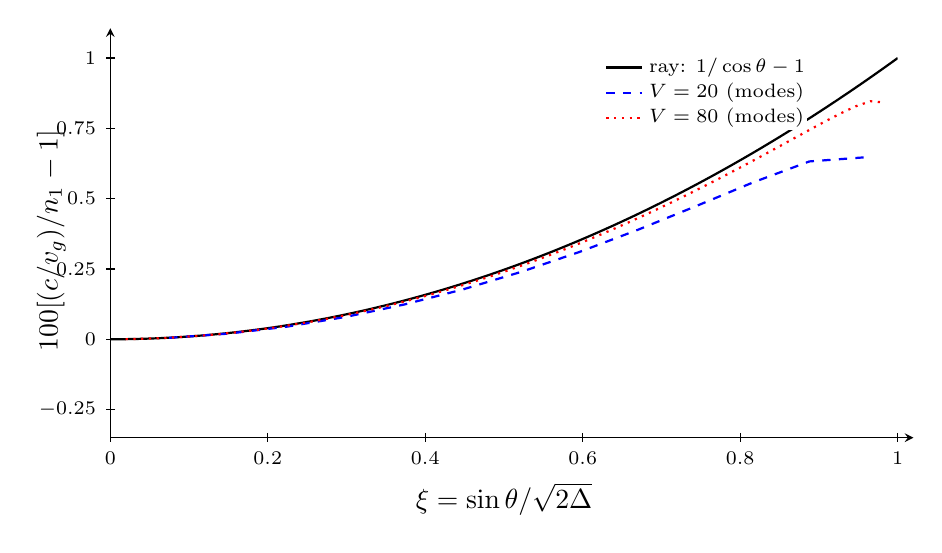
\begin{tikzpicture}[x=1cm,y=1cm,>=stealth]
\draw[->] (0,0)--(10.2,0);
\draw[->] (0,0)--(0,5.2);
\draw (0.00000,.06)--(0.00000,-.06) node[below] {\scriptsize $0$};
\draw (2.00000,.06)--(2.00000,-.06) node[below] {\scriptsize $0.2$};
\draw (4.00000,.06)--(4.00000,-.06) node[below] {\scriptsize $0.4$};
\draw (6.00000,.06)--(6.00000,-.06) node[below] {\scriptsize $0.6$};
\draw (8.00000,.06)--(8.00000,-.06) node[below] {\scriptsize $0.8$};
\draw (10.00000,.06)--(10.00000,-.06) node[below] {\scriptsize $1$};
\draw (.06,0.35714)--(-.06,0.35714) node[left] {\scriptsize $-0.25$};
\draw (.06,1.25000)--(-.06,1.25000) node[left] {\scriptsize $0$};
\draw (.06,2.14286)--(-.06,2.14286) node[left] {\scriptsize $0.25$};
\draw (.06,3.03571)--(-.06,3.03571) node[left] {\scriptsize $0.5$};
\draw (.06,3.92857)--(-.06,3.92857) node[left] {\scriptsize $0.75$};
\draw (.06,4.82143)--(-.06,4.82143) node[left] {\scriptsize $1$};
\node[below] at (5.0,-.45) {$\xi=\sin\theta/\sqrt{2\Delta}$};
\node[rotate=90] at (-.75,2.5) {$100[(c/v_g)/n_1-1]$};
\begin{scope}
\clip (0,0) rectangle (10,5);
\draw[black,thick] plot coordinates {(0.000000,1.250000) (0.033333,1.250039) (0.066667,1.250156) (0.100000,1.250352) (0.133333,1.250626) (0.166667,1.250977) (0.200000,1.251407) (0.233333,1.251916) (0.266667,1.252502) (0.300000,1.253167) (0.333333,1.253910) (0.366667,1.254731) (0.400000,1.255630) (0.433333,1.256607) (0.466667,1.257663) (0.500000,1.258797) (0.533333,1.260009) (0.566667,1.261299) (0.600000,1.262667) (0.633333,1.264114) (0.666667,1.265639) (0.700000,1.267242) (0.733333,1.268924) (0.766667,1.270683) (0.800000,1.272521) (0.833333,1.274437) (0.866667,1.276431) (0.900000,1.278504) (0.933333,1.280655) (0.966667,1.282884) (1.000000,1.285191) (1.033333,1.287576) (1.066667,1.290040) (1.100000,1.292582) (1.133333,1.295203) (1.166667,1.297901) (1.200000,1.300678) (1.233333,1.303533) (1.266667,1.306467) (1.300000,1.309479) (1.333333,1.312569) (1.366667,1.315737) (1.400000,1.318984) (1.433333,1.322309) (1.466667,1.325712) (1.500000,1.329194) (1.533333,1.332754) (1.566667,1.336393) (1.600000,1.340109) (1.633333,1.343904) (1.666667,1.347778) (1.700000,1.351730) (1.733333,1.355760) (1.766667,1.359869) (1.800000,1.364056) (1.833333,1.368322) (1.866667,1.372666) (1.900000,1.377088) (1.933333,1.381589) (1.966667,1.386168) (2.000000,1.390826) (2.033333,1.395562) (2.066667,1.400377) (2.100000,1.405270) (2.133333,1.410241) (2.166667,1.415292) (2.200000,1.420420) (2.233333,1.425628) (2.266667,1.430913) (2.300000,1.436278) (2.333333,1.441720) (2.366667,1.447242) (2.400000,1.452842) (2.433333,1.458520) (2.466667,1.464278) (2.500000,1.470113) (2.533333,1.476028) (2.566667,1.482021) (2.600000,1.488093) (2.633333,1.494243) (2.666667,1.500472) (2.700000,1.506780) (2.733333,1.513166) (2.766667,1.519631) (2.800000,1.526175) (2.833333,1.532798) (2.866667,1.539499) (2.900000,1.546279) (2.933333,1.553138) (2.966667,1.560076) (3.000000,1.567092) (3.033333,1.574188) (3.066667,1.581362) (3.100000,1.588615) (3.133333,1.595947) (3.166667,1.603357) (3.200000,1.610847) (3.233333,1.618415) (3.266667,1.626063) (3.300000,1.633789) (3.333333,1.641595) (3.366667,1.649479) (3.400000,1.657442) (3.433333,1.665484) (3.466667,1.673605) (3.500000,1.681806) (3.533333,1.690085) (3.566667,1.698443) (3.600000,1.706881) (3.633333,1.715397) (3.666667,1.723993) (3.700000,1.732668) (3.733333,1.741422) (3.766667,1.750255) (3.800000,1.759167) (3.833333,1.768159) (3.866667,1.777229) (3.900000,1.786379) (3.933333,1.795608) (3.966667,1.804917) (4.000000,1.814305) (4.033333,1.823772) (4.066667,1.833318) (4.100000,1.842944) (4.133333,1.852649) (4.166667,1.862433) (4.200000,1.872297) (4.233333,1.882240) (4.266667,1.892263) (4.300000,1.902365) (4.333333,1.912547) (4.366667,1.922808) (4.400000,1.933149) (4.433333,1.943569) (4.466667,1.954069) (4.500000,1.964648) (4.533333,1.975307) (4.566667,1.986046) (4.600000,1.996864) (4.633333,2.007762) (4.666667,2.018740) (4.700000,2.029797) (4.733333,2.040934) (4.766667,2.052151) (4.800000,2.063448) (4.833333,2.074824) (4.866667,2.086280) (4.900000,2.097816) (4.933333,2.109432) (4.966667,2.121128) (5.000000,2.132904) (5.033333,2.144760) (5.066667,2.156695) (5.100000,2.168711) (5.133333,2.180807) (5.166667,2.192982) (5.200000,2.205238) (5.233333,2.217574) (5.266667,2.229990) (5.300000,2.242486) (5.333333,2.255062) (5.366667,2.267719) (5.400000,2.280455) (5.433333,2.293272) (5.466667,2.306170) (5.500000,2.319147) (5.533333,2.332205) (5.566667,2.345343) (5.600000,2.358561) (5.633333,2.371860) (5.666667,2.385240) (5.700000,2.398699) (5.733333,2.412239) (5.766667,2.425860) (5.800000,2.439561) (5.833333,2.453343) (5.866667,2.467206) (5.900000,2.481149) (5.933333,2.495172) (5.966667,2.509276) (6.000000,2.523461) (6.033333,2.537727) (6.066667,2.552074) (6.100000,2.566501) (6.133333,2.581009) (6.166667,2.595598) (6.200000,2.610268) (6.233333,2.625018) (6.266667,2.639850) (6.300000,2.654762) (6.333333,2.669756) (6.366667,2.684830) (6.400000,2.699986) (6.433333,2.715223) (6.466667,2.730540) (6.500000,2.745939) (6.533333,2.761419) (6.566667,2.776981) (6.600000,2.792623) (6.633333,2.808347) (6.666667,2.824152) (6.700000,2.840039) (6.733333,2.856006) (6.766667,2.872056) (6.800000,2.888186) (6.833333,2.904398) (6.866667,2.920692) (6.900000,2.937067) (6.933333,2.953523) (6.966667,2.970062) (7.000000,2.986682) (7.033333,3.003383) (7.066667,3.020166) (7.100000,3.037031) (7.133333,3.053978) (7.166667,3.071006) (7.200000,3.088117) (7.233333,3.105309) (7.266667,3.122583) (7.300000,3.139939) (7.333333,3.157377) (7.366667,3.174897) (7.400000,3.192499) (7.433333,3.210183) (7.466667,3.227949) (7.500000,3.245797) (7.533333,3.263728) (7.566667,3.281740) (7.600000,3.299835) (7.633333,3.318013) (7.666667,3.336272) (7.700000,3.354614) (7.733333,3.373039) (7.766667,3.391545) (7.800000,3.410135) (7.833333,3.428806) (7.866667,3.447561) (7.900000,3.466398) (7.933333,3.485317) (7.966667,3.504319) (8.000000,3.523404) (8.033333,3.542572) (8.066667,3.561823) (8.100000,3.581156) (8.133333,3.600572) (8.166667,3.620071) (8.200000,3.639653) (8.233333,3.659318) (8.266667,3.679066) (8.300000,3.698897) (8.333333,3.718811) (8.366667,3.738809) (8.400000,3.758889) (8.433333,3.779053) (8.466667,3.799300) (8.500000,3.819630) (8.533333,3.840044) (8.566667,3.860541) (8.600000,3.881122) (8.633333,3.901786) (8.666667,3.922533) (8.700000,3.943364) (8.733333,3.964279) (8.766667,3.985277) (8.800000,4.006359) (8.833333,4.027525) (8.866667,4.048774) (8.900000,4.070108) (8.933333,4.091525) (8.966667,4.113026) (9.000000,4.134611) (9.033333,4.156280) (9.066667,4.178033) (9.100000,4.199871) (9.133333,4.221792) (9.166667,4.243797) (9.200000,4.265887) (9.233333,4.288061) (9.266667,4.310319) (9.300000,4.332662) (9.333333,4.355089) (9.366667,4.377601) (9.400000,4.400197) (9.433333,4.422877) (9.466667,4.445643) (9.500000,4.468492) (9.533333,4.491427) (9.566667,4.514446) (9.600000,4.537550) (9.633333,4.560739) (9.666667,4.584013) (9.700000,4.607371) (9.733333,4.630815) (9.766667,4.654343) (9.800000,4.677957) (9.833333,4.701656) (9.866667,4.725440) (9.900000,4.749309) (9.933333,4.773264) (9.966667,4.797303) (10.000000,4.821429)};
\draw[blue,dashed,thick] plot coordinates {(0.747965,1.267806) (1.495728,1.321164) (2.243078,1.409876) (2.989782,1.533587) (3.735570,1.691719) (4.480119,1.883370) (5.223013,2.107135) (5.963700,2.360745) (6.701386,2.640360) (7.434848,2.938901) (8.161980,3.241467) (8.878457,3.508351) (9.571652,3.559818)};
\draw[red,dotted,thick] plot coordinates {(0.193925,1.251291) (0.387850,1.255162) (0.581772,1.261615) (0.775692,1.270649) (0.969609,1.282263) (1.163520,1.296459) (1.357426,1.313235) (1.551326,1.332592) (1.745218,1.354529) (1.939102,1.379045) (2.132976,1.406141) (2.326840,1.435817) (2.520692,1.468070) (2.714531,1.502901) (2.908356,1.540309) (3.102165,1.580291) (3.295958,1.622848) (3.489732,1.667977) (3.683487,1.715676) (3.877221,1.765943) (4.070932,1.818775) (4.264618,1.874168) (4.458277,1.932117) (4.651908,1.992619) (4.845507,2.055667) (5.039073,2.121255) (5.232604,2.189374) (5.426095,2.260013) (5.619543,2.333163) (5.812946,2.408808) (6.006300,2.486932) (6.199599,2.567516) (6.392839,2.650535) (6.586015,2.735960) (6.779119,2.823755) (6.972145,2.913878) (7.165085,3.006275) (7.357928,3.100876) (7.550663,3.197598) (7.743275,3.296328) (7.935748,3.396924) (8.128062,3.499189) (8.320188,3.602859) (8.512094,3.707556) (8.703734,3.812724) (8.895046,3.917499) (9.085940,4.020451) (9.276277,4.118977) (9.465819,4.207656) (9.654101,4.272387) (9.839876,4.255467)};
\end{scope}
\draw[black,thick] (6.3,4.7)--(6.75,4.7);
\node[right,fill=white,inner sep=1pt] at (6.8,4.7) {\scriptsize ray: $1/\cos\theta-1$};
\draw[blue,dashed,thick] (6.3,4.38)--(6.75,4.38);
\node[right,fill=white,inner sep=1pt] at (6.8,4.38) {\scriptsize $V=20$ (modes)};
\draw[red,dotted,thick] (6.3,4.0600000000000005)--(6.75,4.0600000000000005);
\node[right,fill=white,inner sep=1pt] at (6.8,4.0600000000000005) {\scriptsize $V=80$ (modes)};
\end{tikzpicture}
\end{center}
The vertical coordinate is the percent excess delay relative to
$n_1L/c$.  Away from the weakly confined highest modes, the points
approach $100(1/\cos\theta-1)$ as $V$ increases.  This is the
step-index optical-path difference of Fig.~8.12b.  Near threshold
the delay is reduced by cladding propagation, so applying the
core-only ray formula there overestimates it.  Even in this
nondispersive model different modes have different delays; material
dispersion would add a further frequency dependence.

\Needspace{5\baselineskip}
\par\bigskip
\noindent\textbf{8.17}\quad Consider the propagating modes in a cylindrical optical fiber waveguide of radius $a$ with a step index of refraction, $n_{1}$ in the core ($\rho<a$) and $n_{2}<n_{1}$ in the cladding ($\rho>a$). Assume that the fields vary as $e^{im\phi+ik_{z}z-i\omega t}$. For bound modes, the fields in the core (cladding) are proportional to ordinary (modified) Bessel functions $J_{\nu}(K_{\nu})$ with appropriate values of $\nu$ and argument, as in (8.128).
\begin{enumerate}
\item[(a)] Show that for $m\neq0$ the eigenvalue relation for the transverse parameter $\gamma_{mn}$ (and $\beta_{mn}$) is
\[
\left(\frac{n_{1}^{2}}{\gamma}\frac{J'_{m}}{J_{m}}+\frac{n_{2}^{2}}{\beta}\frac{K'_{m}}{K_{m}}\right)\!\left(\frac{1}{\gamma}\frac{J'_{m}}{J_{m}}+\frac{1}{\beta}\frac{K'_{m}}{K_{m}}\right)
=\frac{m^{2}}{a^{2}}\left(\frac{n_{1}^{2}}{\gamma^{2}}+\frac{n_{2}^{2}}{\beta^{2}}\right)\!\left(\frac{1}{\gamma^{2}}+\frac{1}{\beta^{2}}\right)
\]
where $\gamma^{2}=n_{1}^{2}\omega^{2}/c^{2}-k_{z}^{2}$ and $\beta^{2}=k_{z}^{2}-n_{2}^{2}\omega^{2}/c^{2}$, while primes indicate derivatives with respect to the argument, and the argument of $J_{m}$ ($K_{m}$) is $\gamma a$ ($\beta a$). The first subscript on $\gamma$ is the azimuthal index $m$; the second designates the $n$th root of the eigenvalue equation for fixed $m$.
\item[(b)] Determine the eigenvalue equation for the $m=0$ modes (TE and TM) and show that the lowest ``cutoff'' frequency corresponds to $V=2.405$, the first root of $J_{0}(x)$, where ``cutoff'' is the frequency below which the guide radiates rather than confines.
\item[(c)] Show that the lowest $HE$ mode ($HE_{11}$) has no cutoff frequency and that for $V\ll1$ the decay parameter $\beta a\approx Ae^{-B/V^{2}}$. Find $A$ and $B$ in terms of $n_{1}$ and $n_{2}$.
\end{enumerate}
\solution

\medskip\noindent\textbf{(a)} Take $\mu=\mu_0$, $\epsilon_i=n_i^2\epsilon_0$ and put
$k_0=\omega/c$.  At $\rho=a$ let the continuous longitudinal
field amplitudes be $E$ and $H$.  In each region Maxwell's equations
give
\[
\mathbf E_t=\frac{i}{g^2}
 (k_z\nabla_tE_z-\omega\mu_0\widehat{\mathbf z}\times\nabla_tH_z),
\quad
\mathbf H_t=\frac{i}{g^2}
 (k_z\nabla_tH_z+\omega\epsilon\widehat{\mathbf z}\times\nabla_tE_z),
\]
with $g^2=\gamma^2$ inside and $g^2=-\beta^2$ outside.
The radial logarithmic derivatives of the longitudinal fields are
$\gamma J_m'/J_m$ and $\beta K_m'/K_m$ respectively.  Define
\[
D=\frac{J_m'}{\gamma J_m}+\frac{K_m'}{\beta K_m},\quad
F=\frac{n_1^2J_m'}{\gamma J_m}+\frac{n_2^2K_m'}{\beta K_m},\quad
C_m=\frac{mk_z}{a}(\gamma^{-2}+\beta^{-2}).
\]
Continuity of $E_\phi,H_\phi$ becomes the two homogeneous equations
\[
C_m E+i\omega\mu_0D H=0,\qquad
 i\omega\epsilon_0F E-C_m H=0.
\]
A nonzero solution requires
\[
FD=\frac{k_z^2}{k_0^2}\frac{m^2}{a^2}
 (\gamma^{-2}+\beta^{-2})^2.
\]
The identity
\[
\frac{n_1^2}{\gamma^2}+\frac{n_2^2}{\beta^2}
=\frac{k_z^2}{k_0^2}(\gamma^{-2}+\beta^{-2})
\]
follows by substituting the definitions of $\gamma,\beta$ and
converts this determinant to the equation in part (a).  The normal
$D,B$ conditions then follow from the tangential Maxwell equations.

\medskip\noindent\textbf{(b)} For $m=0$ the two equations decouple.  With $u=\gamma a$,
$w=\beta a$, $u^2+w^2=V^2$, they are
\[
\boxed{\frac{J_0'(u)}{uJ_0(u)}+
 \frac{K_0'(w)}{wK_0(w)}=0\quad(\mathrm{TE}),}
\]
\[
\boxed{n_1^2\frac{J_0'(u)}{uJ_0(u)}+
 n_2^2\frac{K_0'(w)}{wK_0(w)}=0\quad(\mathrm{TM}).}
\]
At loss of confinement, $w\downarrow0$ and
$K_0'(w)/(wK_0(w))\sim-1/[w^2(-\log(w/2)-\gamma_E)]$
diverges negatively.  Cancellation requires the positive pole of
the $J_0$ term, with $u$ approaching a zero of $J_0$ from above.
The lowest threshold is therefore
\[
\boxed{V_t=x_{01}=2.4048255577\ldots .}
\]

\medskip\noindent\textbf{(c)} For the fundamental hybrid mode put $m=1$, and abbreviate
$S=n_1^2+n_2^2$,
$A_u=J_1'(u)/(uJ_1(u))$, $B_w=K_1'(w)/(wK_1(w))$.
The determinant in dimensionless form is
\[
(n_1^2A_u+n_2^2B_w)(A_u+B_w)
=(n_1^2/u^2+n_2^2/w^2)(1/u^2+1/w^2).
\]
For $w\ll u\ll1$, start with
\[
J_1(u)=\frac u2-\frac{u^3}{16}+\frac{u^5}{384}+O(u^7),
\qquad
K_1(w)=\frac1w+\frac w2
 \left[\log(w/2)+\gamma_E-\frac12\right]+O(w^3\log w).
\]
Differentiating and dividing these series gives
\[
B_w=-w^{-2}-L+O(w^2L^2),\quad L=-\log(w/2)-\gamma_E,
\qquad A_u=u^{-2}-\tfrac14-\tfrac{u^2}{96}+O(u^4).
\]
The $w^{-4}$ terms cancel identically. The $w^{-2}$ coefficients
on the left and right are $2n_2^2L-SA_u$ and $S/u^2$.
Equating them gives
\[
2n_2^2L=S(A_u+u^{-2})
=S\left(\frac2{u^2}-\frac14-\frac{u^2}{96}+\cdots\right).
\]
As $u^2=V^2-w^2$ and $w$ is exponentially small, this becomes
\[
\log(w/2)=-\gamma_E-\frac{S}{n_2^2V^2}
 +\frac{S}{8n_2^2}+O(V^2).
\]
Exponentiating yields
\[
\boxed{\beta a\sim A\exp(-B/V^2),\qquad
 A=2\exp\!\left[-\gamma_E+\frac{n_1^2+n_2^2}{8n_2^2}\right],
 \quad B=\frac{n_1^2+n_2^2}{n_2^2}.}
\]
The relative correction to this leading expression is $O(V^2)$.
There is a positive but exponentially small decay constant at
arbitrarily small positive $V$: the $HE_{11}$ branch has no
positive cutoff.  Its very long cladding tail should not be confused
with a well-confined ray.  The supplementary code solves a
cancellation-free form of the determinant in $\log w$ and checks
this limit; for $n_1=1.5,n_2=1,V=0.3$ it finds
$\log w=-35.58739754$, versus $-35.58892960$ from the asymptote.

\Needspace{5\baselineskip}
\par\bigskip
\noindent\textbf{8.18}\quad\begin{enumerate}
\item[(a)] From the use of Green's theorem in two dimensions show that the TM and TE modes in a waveguide defined by the boundary-value problems (8.34) and (8.36) are orthogonal in the sense that
\[
\int_{A}E_{z\lambda}E_{z\mu}\;da=0\qquad\text{for }\lambda\neq\mu
\]
for TM modes, and a corresponding relation for $H_{z}$ for TE modes.
\item[(b)] Prove that the relations (8.131)--(8.134) form a consistent set of normalization conditions for the fields, including the circumstances when $\lambda$ is a TM mode and $\mu$ is a TE mode.
\end{enumerate}
\solution

\medskip\noindent\textbf{(a)} Use a uniform real $\epsilon,\mu$ and a perfectly conducting
boundary.  Choose real scalar eigenfunctions of
$-\nabla_t^2$, Dirichlet for TM and Neumann for TE.
For two scalar eigenfunctions $f_\lambda,f_\mu$, Green's identity
is
\[
(\gamma_\lambda^2-\gamma_\mu^2)
 \int_A f_\lambda f_\mu\,da
=\oint_{\partial A}
 (f_\lambda\partial_nf_\mu-f_\mu\partial_nf_\lambda)\,dl=0.
\]
Thus different eigenvalues are orthogonal.  Within a degenerate
eigenspace choose an orthogonal basis; the eigenvalue equation
alone does not make arbitrary degenerate linear combinations
orthogonal.  This establishes the stated relation for $E_z$ and
its TE counterpart for $H_z$.  The constant Neumann scalar is
excluded because it produces no TE field.

\medskip\noindent\textbf{(b)} Let $D_\lambda,N_\lambda$ be Dirichlet and nonconstant Neumann
scalars normalized to $\int_A f_\lambda f_\mu\,da=\delta_{\lambda\mu}$.
Integration by parts gives
\[
\int_A\nabla_tf_\lambda\cdot\nabla_tf_\mu\,da
=\gamma_\mu^2\delta_{\lambda\mu}.
\]
The normalized transverse electric fields can therefore be chosen as
\[
\mathbf E_\lambda^{\rm TM}=\frac{\nabla_tD_\lambda}{\gamma_\lambda},
\qquad
\mathbf E_\lambda^{\rm TE}=
 -\frac{\widehat{\mathbf z}\times\nabla_tN_\lambda}{\gamma_\lambda}.
\]
Within either family their inner product is $\delta_{\lambda\mu}$.
For a mixed pair, $\nabla_t\cdot(\widehat{\mathbf z}\times\nabla_tN)=0$
and $D=0$ on the wall imply
\[
\int_A\nabla_tD\cdot(\widehat{\mathbf z}\times\nabla_tN)\,da
=\oint_{\partial A}D(\widehat{\mathbf z}\times\nabla_tN)
 \cdot\mathbf n\,dl=0.
\]
This proves (8.131) for all pairs, including accidental degeneracy
between TE and TM families.

With $k_\lambda^2=\omega^2\mu\epsilon-\gamma_\lambda^2$,
\[
\mathbf H_\lambda=\frac{\widehat{\mathbf z}\times\mathbf E_\lambda}
 {Z_\lambda},\qquad
Z_{\rm TM}=\frac{k_\lambda}{\omega\epsilon},\quad
Z_{\rm TE}=\frac{\omega\mu}{k_\lambda},
\]
so the remaining transverse bilinear integrals follow directly:
\[
\int_A\mathbf H_\lambda\cdot\mathbf H_\mu\,da
 =\frac{\delta_{\lambda\mu}}{Z_\lambda^2},\qquad
\frac12\int_A(\mathbf E_\lambda\times\mathbf H_\mu)
 \cdot\widehat{\mathbf z}\,da
 =\frac{\delta_{\lambda\mu}}{2Z_\lambda}.
\]
Finally $\nabla\cdot\mathbf E=\nabla\cdot\mathbf H=0$ gives
\[
E_{z\lambda}^{\rm TM}=-\frac{i\gamma_\lambda}{k_\lambda}D_\lambda,
\qquad
H_{z\lambda}^{\rm TE}=-\frac{i\gamma_\lambda}{k_\lambda Z_\lambda}N_\lambda,
\]
and consequently
\[
\boxed{\int_A E_{z\lambda}E_{z\mu}\,da
 =-\frac{\gamma_\lambda^2}{k_\lambda^2}\delta_{\lambda\mu},
\qquad
\int_A H_{z\lambda}H_{z\mu}\,da
 =-\frac{\gamma_\lambda^2}{k_\lambda^2Z_\lambda^2}\delta_{\lambda\mu}.}
\]
These are exactly the signs and factors of (8.134): the textbook
uses bilinear products, without complex conjugation, and longitudinal
fields are imaginary when the transverse electric field is real.
For a propagating mode $Z$ is positive and the power of amplitude
$A$ is $|A|^2/(2Z)$.  For an evanescent mode the bilinear equations
remain algebraic normalization identities, while the actual mean
power uses $\tfrac12\operatorname{Re}(\mathbf E\times\mathbf H^*)$
and is zero for a single decaying mode.  Exactly at cutoff,
$k=0$, these field conventions must be interpreted by a rescaled
limit rather than by division by zero.

\Needspace{5\baselineskip}
\par\bigskip
\noindent\textbf{8.19}\quad The figure shows a cross-sectional view of an infinitely long rectangular waveguide with the center conductor of a coaxial line extending vertically a distance $h$ into its interior at $z=0$. The current along the probe oscillates sinusoidally in time with frequency $\omega$, and its variation in space can be approximated as $I(y)=I_{0}\sin[(\omega/c)(h-y)]$. The thickness of the probe can be neglected. The frequency is such that only the $\mathrm{TE}_{10}$ mode can propagate in the guide.

\begin{center}
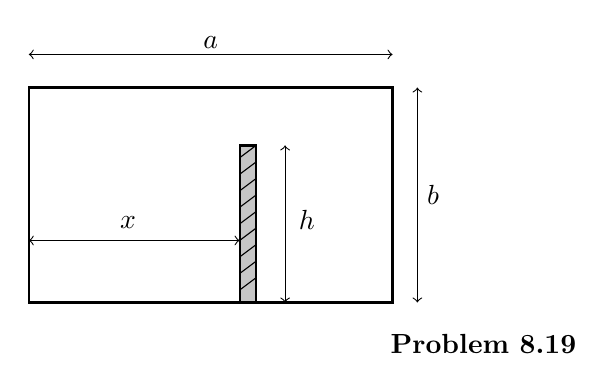
\begin{tikzpicture}[scale=1.05]
  % guide cross-section
  \draw[thick] (0,0) rectangle (4.4,2.6);
  \draw[<->] (0,3.0) -- (4.4,3.0);
  \node[above] at (2.2,2.95) {$a$};
  \draw[<->] (4.7,0) -- (4.7,2.6);
  \node[right] at (4.7,1.3) {$b$};
  % probe from bottom
  \fill[gray!45] (2.55,0) rectangle (2.75,1.9);
  \draw[thick] (2.55,0) rectangle (2.75,1.9);
  \foreach \y in {0.15,0.35,...,1.8}{\draw (2.55,\y) -- (2.75,\y+0.15);}
  % h dimension
  \draw[<->] (3.1,0) -- (3.1,1.9);
  \node[right] at (3.15,1.0) {$h$};
  % x dimension from left wall
  \draw[<->] (0,0.75) -- (2.55,0.75);
  \node[above] at (1.2,0.78) {$x$};
  \node at (5.5,-0.5) {\textbf{Problem 8.19}};
\end{tikzpicture}
\end{center}

\begin{enumerate}
\item[(a)] Calculate the amplitudes for excitation of both TE and TM modes for all $(m,n)$ and show how the amplitudes depend on $m$ and $n$ for $m,n\gg1$ for a fixed frequency $\omega$.
\item[(b)] For the propagating mode show that the power radiated in the positive $z$ direction is
\[
P=\frac{\mu c^{2}I_{0}^{2}}{\omega kab}\sin^{2}\!\left(\frac{\pi X}{a}\right)\sin^{4}\!\left(\frac{\omega h}{2c}\right)
\]
with an equal amount in the opposite direction. Here $k$ is the wave number for the $\mathrm{TE}_{10}$ mode.
\item[(c)] Discuss the modifications that occur if the guide, instead of running off to infinity in both directions, is terminated with a perfectly conducting surface at $z=L$. What values of $L$ will maximize the power flow for a fixed current $I_{0}$? What is the radiation resistance of the probe (defined as the ratio of power flow to one-half the square of the current at the base of the probe) at maximum?
\end{enumerate}
\solution

\medskip\noindent\textbf{(a)} Use $X$ for the horizontal probe position marked $x$ in the sketch,
and $k_0=\omega/c$.  The prescribed current is
\[
\mathbf J=\widehat{\mathbf y} I_0\sin[k_0(h-y)]
 \delta(x-X)\delta(z),\qquad 0<y<h.
\]
Normalize the transverse electric fields to unit squared integral,
as in (8.131).  Put
\[
q_m=m\pi/a,\quad q_n=n\pi/b,\quad
\gamma_{mn}^2=q_m^2+q_n^2,\quad
k_{mn}=\sqrt{k_0^2-\gamma_{mn}^2},
\]
choosing $k>0$ for propagation and $\operatorname{Im}k>0$ for decay.
With $N_{mn}=\sqrt{(2-\delta_{m0})(2-\delta_{n0})/(ab)}$,
the components needed in the source integral are
\[
E_{y,mn}^{\rm TM}=N_{mn}\frac{q_n}{\gamma_{mn}}
 \sin(q_mx)\cos(q_ny),\qquad
E_{y,mn}^{\rm TE}=N_{mn}\frac{q_m}{\gamma_{mn}}
 \sin(q_mx)\cos(q_ny).
\]
TM requires $m,n\geq1$; TE permits either index to be zero but
excludes $(0,0)$.  These signs agree with (8.135)--(8.136).
The product-to-sum identity gives the elementary source integral:
\[
F_n=\int_0^h\sin[k_0(h-y)]\cos(q_ny)\,dy
 =\frac{\cos(q_nh)-\cos(k_0h)}2
 \left(\frac1{k_0-q_n}+\frac1{k_0+q_n}\right).
\]
Combining the fractions,
\[
F_n=\frac{k_0[\cos(q_nh)-\cos(k_0h)]}{k_0^2-q_n^2}.
\]
When $q_n=k_0$, its continuous limit is
$F_n=(h/2)\sin(k_0h)$, so the apparent denominator singularity is
removable.

Reciprocity, (8.146), gives
$A_\lambda^{(\pm)}=-(Z_\lambda/2)\int\mathbf J\cdot
\mathbf E_\lambda^{(\mp)}d^3x$.
The transverse source at $z=0$ therefore excites equal amplitudes
in both directions:
\[
\boxed{A_{mn}^{{\rm TM},\pm}
=-\frac{I_0Z_{mn}^{\rm TM}}2 N_{mn}\frac{q_n}{\gamma_{mn}}
 \sin(q_mX)F_n,\qquad Z_{mn}^{\rm TM}=\frac{k_{mn}}{\omega\epsilon},}
\]
\[
\boxed{A_{mn}^{{\rm TE},\pm}
=-\frac{I_0Z_{mn}^{\rm TE}}2 N_{mn}\frac{q_m}{\gamma_{mn}}
 \sin(q_mX)F_n,\qquad Z_{mn}^{\rm TE}=\frac{\omega\mu}{k_{mn}}.}
\]
In particular all $m=0$ TE amplitudes vanish.  At fixed $\omega$
and $m,n\gg1$, $k\sim i\gamma$ and $F_n=O(n^{-2})$.
Keeping the oscillating trigonometric factors understood,
\[
A^{\rm TM}_{mn}=O(n^{-1}),\qquad
A^{\rm TE}_{mn}=O\!\left(\frac{m}{(m^2+n^2)n^2}\right).
\]
When both indices grow at a fixed ratio these are $O(M^{-1})$
and $O(M^{-3})$, respectively.  Some coefficients vanish faster
or exactly by symmetry.  These are source-plane amplitudes; at
$z\ne0$ the high modes also contain $e^{-\gamma|z|}$.

\medskip\noindent\textbf{(b)} For $\mathrm{TE}_{10}$,
$F_0=2\sin^2(k_0h/2)/k_0$, $N_{10}=\sqrt{2/(ab)}$, so
\[
A_{10}^{\pm}=-\frac{ZI_0}{k_0}\sqrt{\frac2{ab}}
 \sin\frac{\pi X}{a}\sin^2\frac{k_0h}{2}.
\]
Since the power in either outgoing wave is $|A_{10}|^2/(2Z)$,
\[
\boxed{P=\frac{ZI_0^2}{abk_0^2}
 \sin^2\frac{\pi X}{a}\sin^4\frac{k_0h}{2}
=\frac{\mu c^2I_0^2}{\omega kab}
 \sin^2\frac{\pi X}{a}\sin^4\frac{\omega h}{2c}.}
\]
Here $I_0$ is a peak phasor amplitude; replace $I_0^2$ by
$|I_0|^2$ if its phase has not been chosen real.

\medskip\noindent\textbf{(c)} A short at $z=L>0$ reflects transverse electric fields with
coefficient $-1$.  Equivalently add a negative image probe at
$z=2L$.  The outgoing amplitude at $z<0$ for each mode is
\[
A_{mn}^{\rm left}=A_{mn}^{-}(1-e^{2ik_{mn}L}).
\]
In $0<z<L$ the field is a standing-wave combination with zero
tangential electric field at the short.  The same image construction
includes the evanescent near fields; for those modes $e^{2ikL}$
is real and decaying.  Only the propagating mode transports power
far to the left, giving
\[
P_{\rm left}=4P\sin^2kL,\qquad
\boxed{L=(2j+1)\pi/(2k),\quad j=0,1,\ldots}
\]
for maxima at fixed prescribed current.  The maximum is $4P$,
compared with total power $2P$ in the unterminated guide.
With $I_{\rm base}=I_0\sin k_0h$, the radiation resistance there is
\[
\boxed{R_{\rm rad,max}=\frac{4P}{|I_{\rm base}|^2/2}
 =\frac{2Z}{abk_0^2}\sin^2\frac{\pi X}{a}
 \tan^2\frac{k_0h}{2}.}
\]
This definition presumes nonzero base current; a prescribed profile
with zero base current cannot be assigned a finite resistance by
that ratio.  A physical source of fixed voltage would also have
its current changed by the reflected wave, whereas the problem
holds $I_0$ fixed.

\Needspace{5\baselineskip}
\par\bigskip
\noindent\textbf{8.20}\quad An infinitely long rectangular waveguide has a coaxial line terminating in the short side of the guide with the thin central conductor forming a semicircular loop of radius $R$ whose center is a height $h$ above the floor of the guide, as shown in the accompanying cross-sectional view. The half-loop is in the plane $z=0$ and its radius $R$ is sufficiently small that the current can be taken as having a constant value $I_{0}$ everywhere on the loop.

\begin{center}
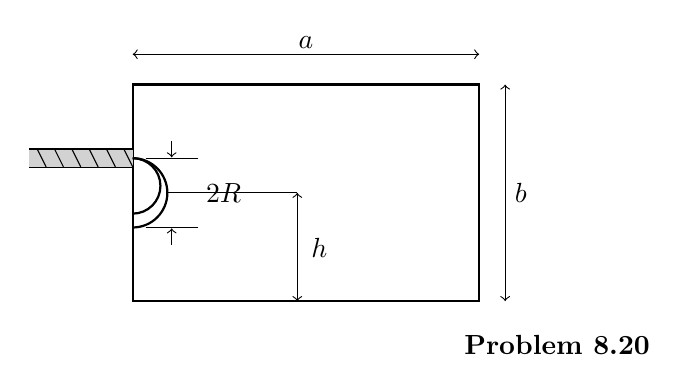
\begin{tikzpicture}[scale=1.1]
  % guide cross-section
  \draw[thick] (0.7,0) rectangle (4.7,2.5);
  \draw[<->] (0.7,2.85) -- (4.7,2.85);
  \node[above] at (2.7,2.8) {$a$};
  \draw[<->] (5.0,0) -- (5.0,2.5);
  \node[right] at (5.0,1.25) {$b$};
  % coax line terminating at the left wall
  \draw[thick] (-0.5,1.55) -- (0.7,1.55);
  \draw[thick] (-0.5,1.75) -- (0.7,1.75);
  \fill[gray!35] (-0.5,1.55) rectangle (0.7,1.75);
  \foreach \x in {-0.4,-0.2,0.0,0.2,0.4,0.6}{\draw (\x,1.75) -- (\x+0.1,1.55);}
  % semicircular half-loop bulging into the guide, vertical diameter 2R
  %  (center at height h = 1.25, ends on the wall at 1.25 +- 0.4)
  \draw[thick] (0.7,1.65) arc (90:-90:0.4);
  \draw[thick] (0.7,1.65) arc (90:-90:0.32);
  % datum lines at the two ends of the diameter, with arrowheads
  \draw (0.85,1.65) -- (1.45,1.65);
  \draw[->] (1.15,1.85) -- (1.15,1.66);
  \draw (0.85,0.85) -- (1.45,0.85);
  \draw[->] (1.15,0.65) -- (1.15,0.84);
  \node at (1.75,1.25) {$2R$};
  % h dimension: floor to the center of the loop
  \draw (1.1,1.25) -- (2.6,1.25);
  \draw[<->] (2.6,0) -- (2.6,1.25);
  \node[right] at (2.65,0.62) {$h$};
  \node at (5.6,-0.5) {\textbf{Problem 8.20}};
\end{tikzpicture}
\end{center}

\begin{enumerate}
\item[(a)] Prove that to the extent that the current is constant around the half-loop, the TM modes are not excited. Give a physical explanation of this lack of excitation.
\item[(b)] Determine the amplitude for the lowest TE mode in the guide and show that its value is independent of the height $h$.
\item[(c)] Show that the power radiated in either direction in the lowest TE mode is
\[
P=\frac{I_{0}^{2}}{16}\,Z\,\frac{a}{b}\left(\frac{\pi R}{a}\right)^{4}
\]
where $Z$ is the wave impedance of the $\mathrm{TE}_{10}$ mode. Here assume $R\ll a,b$.
\end{enumerate}
\solution

\medskip\noindent\textbf{(a)} The mode coefficient for the filament is
\[
A_\lambda^{\pm}=-\frac{Z_\lambda I_0}{2}
 \int_{\rm arc}\mathbf E_{t\lambda}\cdot d\boldsymbol\ell.
\]
For TM modes $\mathbf E_t=\nabla_tD/\gamma$, where $D$ vanishes
on the metal boundary.  Consequently
\[
\int_{\rm arc}\mathbf E_t^{\rm TM}\cdot d\boldsymbol\ell
=\frac{D(\hbox{end})-D(\hbox{start})}{\gamma}=0.
\]
This proves the absence of every TM mode, including evanescent
ones, without a small-$R$ expansion.  The constant current together
with its return in the wall forms a solenoidal transverse loop.
It has magnetic circulation and no varying line charge along the
arc, so its transverse overlap with a gradient field is zero.
If the current varied around the loop, integration by parts would
leave a term involving that variation and TM excitation could occur.

\medskip\noindent\textbf{(b)} Choose the direction of current to increase
$\vartheta$ in
\[
x=R\cos\vartheta,\qquad y=h+R\sin\vartheta,
\qquad -\pi/2\leq\vartheta\leq\pi/2.
\]
For TE$_{10}$, $E_y=\sqrt{2/(ab)}\sin(\pi x/a)$ and $E_x=0$.
Its overlap is independent of $h$:
\begin{align*}
\int_{\rm arc}\mathbf E_t\cdot d\boldsymbol\ell
 &=\sqrt{\frac2{ab}}R\int_{-\pi/2}^{\pi/2}
 \cos\vartheta\sin\!\left(\frac{\pi R}{a}\cos\vartheta\right)d\vartheta\\
 &=\sqrt{\frac2{ab}}\,\pi R J_1(\pi R/a).
\end{align*}
The last identity follows by differentiating
$\int_{-\pi/2}^{\pi/2}\cos(t\cos\vartheta)d\vartheta=\pi J_0(t)$.
Thus, for constant current, the exact coefficient is
\[
\boxed{A_{10}^{\pm}=-\frac{ZI_0}2\sqrt{\frac2{ab}}
 \pi R J_1(\pi R/a).}
\]
Reversing the loop orientation reverses its sign but not its power.
For $R\ll a,b$, $J_1(t)=t/2+O(t^3)$, and therefore
\[
A_{10}^{\pm}=-ZI_0\sqrt{\frac2{ab}}\frac{\pi^2R^2}{4a}
 [1+O(R^2/a^2)].
\]
\medskip\noindent\textbf{(c)} The power in either direction is
\[
\boxed{P=\frac{|A_{10}|^2}{2Z}
 =\frac{I_0^2}{16}Z\frac ab
 \left(\frac{\pi R}{a}\right)^4
 [1+O(R^2/a^2)].}
\]
The exact constant-current result before this expansion is
$P=ZI_0^2\pi^2R^2J_1^2(\pi R/a)/(4ab)$.
The independence of $h$ follows from the absence of any $y$
dependence in the TE$_{10}$ field, provided the entire loop remains
inside the guide.

\Needspace{5\baselineskip}
\par\bigskip
\noindent\textbf{8.21}\quad A hollow metallic waveguide with a distortion in the form of a localized bend or increase in cross section can support nonpropagating (``bound state'') configurations of fields in the vicinity of the distortion. Consider a rectangular guide that has its distortion confined to a plane, as shown in the figure, and $\mathrm{TE}_{10}$ as its lowest propagating mode, with perpendicular electric field $E_{\perp}=\psi$. On either side of the distortion the guide is straight and of width $a$. Without distortion, $\psi=E_{0}\sin(\pi y/a)\exp(\pm ikz)$, where $k^{2}=(\omega/c)^{2}-(\pi/a)^{2}$. The distortion is described by a curvature $\kappa(s)=1/R(s)$ and a width $w(s)$. Locally the element of area in the plane is $dA=h(s,t)\;ds\;dt$, where $s$ is the length along the guide wall and $t$ the transverse coordinate, as shown in the figure, and $h(s,t)=1-\kappa(s)t$. In terms of $s$ and $t$ the Laplacian is
\[
\nabla^{2}\psi=\frac{1}{h}\frac{\partial}{\partial t}\left(h\frac{\partial\psi}{\partial t}\right)+\frac{1}{h}\frac{\partial}{\partial s}\left(\frac{1}{h}\frac{\partial\psi}{\partial s}\right)
\]
If the distortions are very small and change slowly in $s$ on the scale of the width $a$, an ansatz for the solution is
\[
\psi(s,t)=\frac{u(s)}{\sqrt{h(s,t)}}\cdot\sin\!\left[\frac{\pi t}{w(s)}\right]
\]
[The factor in the denominator is equivalent to the factor $\rho^{-1/2}$ familiar from Bessel functions that converts the radial part of the Laplacian in polar coordinates to a simple second partial derivative (plus an additional term without derivatives).]
\begin{enumerate}
\item[(a)] Show that substitution of the ansatz into the two-dimensional wave equation, $(\nabla^{2}+\omega^{2}/c^{2})\psi=0$, leads to the equation for $u(s)$,
\[
\frac{d^{2}u}{ds^{2}}+[k^{2}-v(s)]u=0\qquad\text{with }v(s)=\pi^{2}\!\left(\frac{1}{w^{2}(s)}-\frac{1}{a^{2}}\right)-\frac{1}{4}\,\kappa^{2}(s)
\]
if small terms are neglected. Interpret $v(s)$ in analogy with the Schr\"odinger equation in one dimension.
\item[(b)] If the distortion is in the form of a bend through an angle $\theta$ with constant radius of curvature $R\gg a$, show that for $\theta a/R\ll1$ \erratum{and $|\theta|\ll1$} there is a ``bound state'' at frequency $\omega_{0}$ where
\[
\omega_{0}^{2}\approx\left(\frac{\pi c}{a}\right)^{2}\!\left[1-\left(\frac{\theta a}{8\pi R}\right)^{2}\right]
\]
\end{enumerate}
\erratum{The additional small-angle assumption is needed for the stated leading coefficient; the finite-angle bound state is treated in the solution.}

References: J.~Goldstone and R.~L. Jaffe, \emph{Phys. Rev. B} \textbf{45}, 14100 (1992); J.~P. Carini, J.~T. Londergan, K.~Mullen, and D.~P. Murdock, \emph{Phys. Rev. B} \textbf{48}, 4503 (1993).

\begin{center}
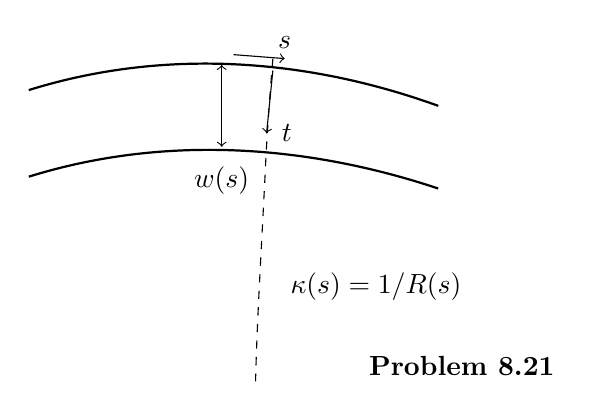
\begin{tikzpicture}[scale=1.0]
  % curved guide walls (gentle bend)
  \draw[thick] (-2.6,1.1) .. controls (-1.0,1.6) and (0.8,1.55) .. (2.6,0.9);
  \draw[thick] (-2.6,0.0) .. controls (-1.0,0.5) and (0.8,0.45) .. (2.6,-0.15);
  % s arrow along top wall
  \draw[->] (0.0,1.55) -- (0.65,1.5) node[above] {$s$};
  % w(s) double arrow between walls near s=0 region
  \draw[<->] (-0.15,1.42) -- (-0.15,0.38);
  \node[below] at (-0.15,0.25) {$w(s)$};
  % t arrow transverse (dashed centerline downward)
  \draw[dashed] (0.5,1.5) .. controls (0.45,0.9) and (0.42,0.45) .. (0.4,0.0)
    .. controls (0.35,-1.0) and (0.3,-1.8) .. (0.28,-2.6);
  \draw[->] (0.5,1.35) -- (0.42,0.55) node[right=2pt] {$t$};
  \node[right] at (0.6,-1.4) {$\kappa(s)=1/R(s)$};
  \node at (2.9,-2.4) {\textbf{Problem 8.21}};
\end{tikzpicture}
\end{center}
\solution

\medskip\noindent\textbf{(a)} Put $f(s,t)=u(s)\sin[\pi t/w(s)]$ and $\psi=h^{-1/2}f$.
At fixed $s$, $h_t=-\kappa$, and direct differentiation gives
\[
\frac1h\partial_t(h\partial_t\psi)
=h^{-1/2}\left(\partial_t^2f+
 \frac{\kappa^2}{4h^2}f\right).
\]
For $|\kappa|a\ll1$, slowly varying width and curvature, and a
longitudinal amplitude varying on scales large compared with $a$,
the longitudinal part can be expanded explicitly as
\[
\frac1h\partial_s(h^{-1}\partial_s\psi)
=h^{-1/2}\left[\frac{f_{ss}}{h^2}
-\frac{2h_s f_s}{h^3}
+\left(\frac{5h_s^2}{4h^4}-\frac{h_{ss}}{2h^3}\right)f\right].
\]
Here $h_s=-t\kappa'$ and $h_{ss}=-t\kappa''$. Writing
$\vartheta=\pi t/w(s)$ also gives
\[
f_{ss}=u''\sin\vartheta+2u'\vartheta_s\cos\vartheta
+u\vartheta_{ss}\cos\vartheta-u\vartheta_s^2\sin\vartheta,
\quad
\vartheta_s=-\frac{\pi t w'}{w^2},\quad
\vartheta_{ss}=-\frac{\pi t w''}{w^2}
+\frac{2\pi t(w')^2}{w^3}.
\]
Discarding these width and curvature derivatives, and replacing
$h^{-2}$ by $1$ in the slow longitudinal derivative term, leaves
$h^{-1/2}u''\sin(\pi t/w)$. These are precisely the stated
adiabatic and small-curvature approximations.
Using $\partial_t^2f=-(\pi/w)^2f$ and $h^{-2}=1+O(\kappa a)$
in the curvature term gives
\[
u''+\left[\frac{\omega^2}{c^2}-\frac{\pi^2}{w^2(s)}
 +\frac{\kappa^2(s)}4\right]u=0.
\]
Separating the straight-guide cutoff gives the stated equation,
\[
\boxed{-u''+v(s)u=k^2u,\qquad
v(s)=\pi^2\left[\frac1{w^2(s)}-\frac1{a^2}\right]
 -\frac{\kappa^2(s)}4.}
\]
It is a one-dimensional Schr\"odinger eigenproblem with energy
$k^2$.  A widening makes the first term attractive; curvature
makes the second term attractive regardless of the direction of
bending.  A localized negative potential in one dimension supports
a bound ground state.  Here $k^2=-q^2<0$ means fields decay in
the straight sections, with frequency below $\pi c/a$; it does
not mean a negative electromagnetic frequency squared.

\medskip\noindent\textbf{(b)} For a bend of constant radius and unchanged width, the reduced
potential is a square well of depth $1/(4R^2)$ and length
$\ell=R|\theta|$.  Smooth end transitions much shorter than $R$
and than $\ell$, but longer than $a$, give the same leading well
limit while preserving the slow-variation assumption of (a).
This smooth-well interpretation requires $a\ll\ell$ as well as
$a\ll R$. With the
origin at its center the even ground-state solution is proportional
to $\cos(bs)$ inside and $e^{-q(|s|-\ell/2)}$ outside, where
\[
b^2=\frac1{4R^2}-q^2,\qquad
\boxed{q=b\tan(b\ell/2).}
\]
For a weak, short well, $b\ell/2\ll1$.  This requires
$|\theta|\ll1$, independently of $a/R$.  Expanding the tangent
then gives
\[
q=\frac{\ell}{8R^2}[1+O(\theta^2)]
=\frac{|\theta|}{8R}[1+O(\theta^2)].
\]
Since $\omega_0^2/c^2=(\pi/a)^2-q^2$, the requested leading
small-angle result is
\[
\boxed{\omega_0^2\simeq\left(\frac{\pi c}{a}\right)^2
 \left[1-\left(\frac{\theta a}{8\pi R}\right)^2\right].}
\]
The retained relative shift is small when $|\theta|a/R\ll1$,
but that condition alone does not justify its coefficient.
This is the reason for the red correction to part (b).
For finite angles the full reduced-model answer remains available:
let $x\in(0,\pi/2)$ solve
\[
\frac{x}{\cos x}=\frac{|\theta|}{4},\qquad
qR=\tfrac12\sin x,\qquad
\omega_0^2=\left(\frac{\pi c}{a}\right)^2-
 \frac{c^2\sin^2x}{4R^2}.
\]
For example $\theta=\pi$ gives $qR=0.2958470340$, whereas
$|\theta|/8=0.3926990817$.  Taking $R/a$ arbitrarily large
satisfies the originally printed $\theta a/R\ll1$ without
removing this discrepancy.  Thus the small-angle requirement is
mathematical, not merely a preference about how tightly the guide
should bend.
